%#!uplatex main.tex

\section{Application}

In this section, we introduce advanced usage of IIS.

\subsection{Render internal area}

\begin{figure}[htbp]
  \center
  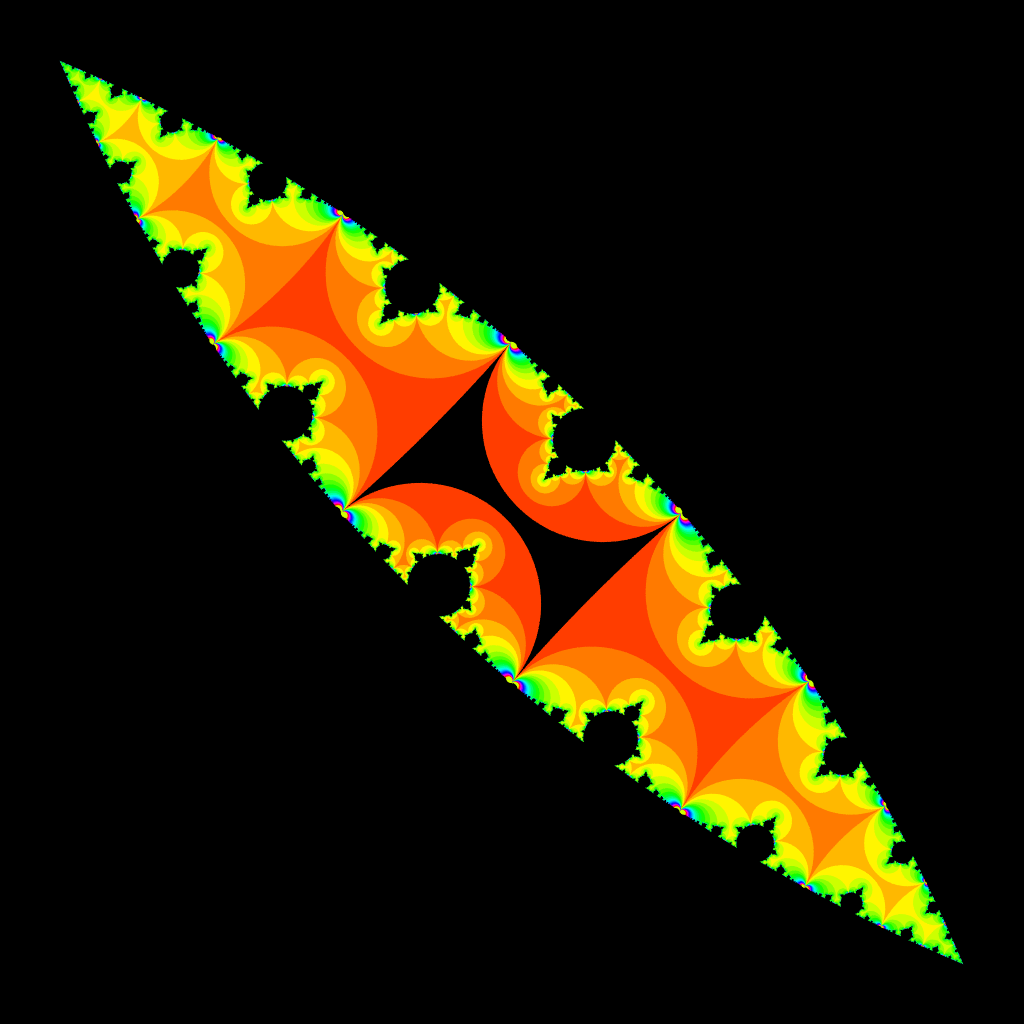
\includegraphics[height=1.35in, keepaspectratio]{img/application/internal/schottky.png}
  \caption{\textit{Edge of the circlte inversion fractal}}
  \label{fig:divideTwo}
 \hspace*{\fill}
\end{figure}

%% 二次元のフラクタルの内側だけを描く.全ての円盤が接していれば極限集合
%% で二分割することができる

In two dimensional circle inversion fractals,
when all of the circles touches each other, the limit set divides plane
into two. See Figure \ref{fig:divideTwo}.
transformed point is outside of the limit set.

We fill a pixel result of IIS, the point moved into inner part of the
resulting fractal.

\subsection{Render Edge of the Circles}

\begin{figure}[htbp]
  \center
  \includegraphics[height=1.35in, keepaspectratio]{img/application/edge/circleEdge.png}
  \caption{\textit{Edge of the circlte inversion fractal}}
  \label{fig:circleEdge}
 \hspace*{\fill}
\end{figure}

We can draw only edges of disks in circle inversion fractals.
We can estimate the distance from the center of the disks using jacobian
of circle inversions.

%% ヤコビアンを累積させていき,最後の円周からの距離を累積させたヤコビア
%% ンで割ることで,円周から点までの距離を得ることができる.

\subsection{Geometrical Representation of M\"obius Transformation Groups}

%% メビウス変換を円や球の反転で定義することによって,より直観的に生成元
%% を得て描画することができる.

In this paper, we mainly use circle or sphere inversions.
We can compose M\"obius transformations by even number of
inversion.
So far, we only use simple circle or sphere inversions.
Other interesting images can be generated using more
complicated M\"obius transformations.
It is known that we can construct any M\"obius transformation out of
inversions.
Thus, we can apply IIS to visualize fractals combining circle inversion
fractals and M\"obius transformation groups.
Moreover, we can tweak parameters of M\"obius transformations by
arranging geometrical objects like circles or lines on the plane.

\subsubsection{Two Dimensionanl Generators}

\begin{figure}[htbp]
 \begin{minipage}[t]{0.5\hsize}
  \begin{minipage}{0.25\hsize}
   \center
   
\includegraphics[ height=1.4in, keepaspectratio]{./img/application/2dGen/infInvEdgedGen.pdf}
   \subcaption{\textit{Generator}}
   \label{fig:infCircleGen}
  \end{minipage}
  \hspace*{\fill}
  \begin{minipage}{0.25\hsize}
   \center
   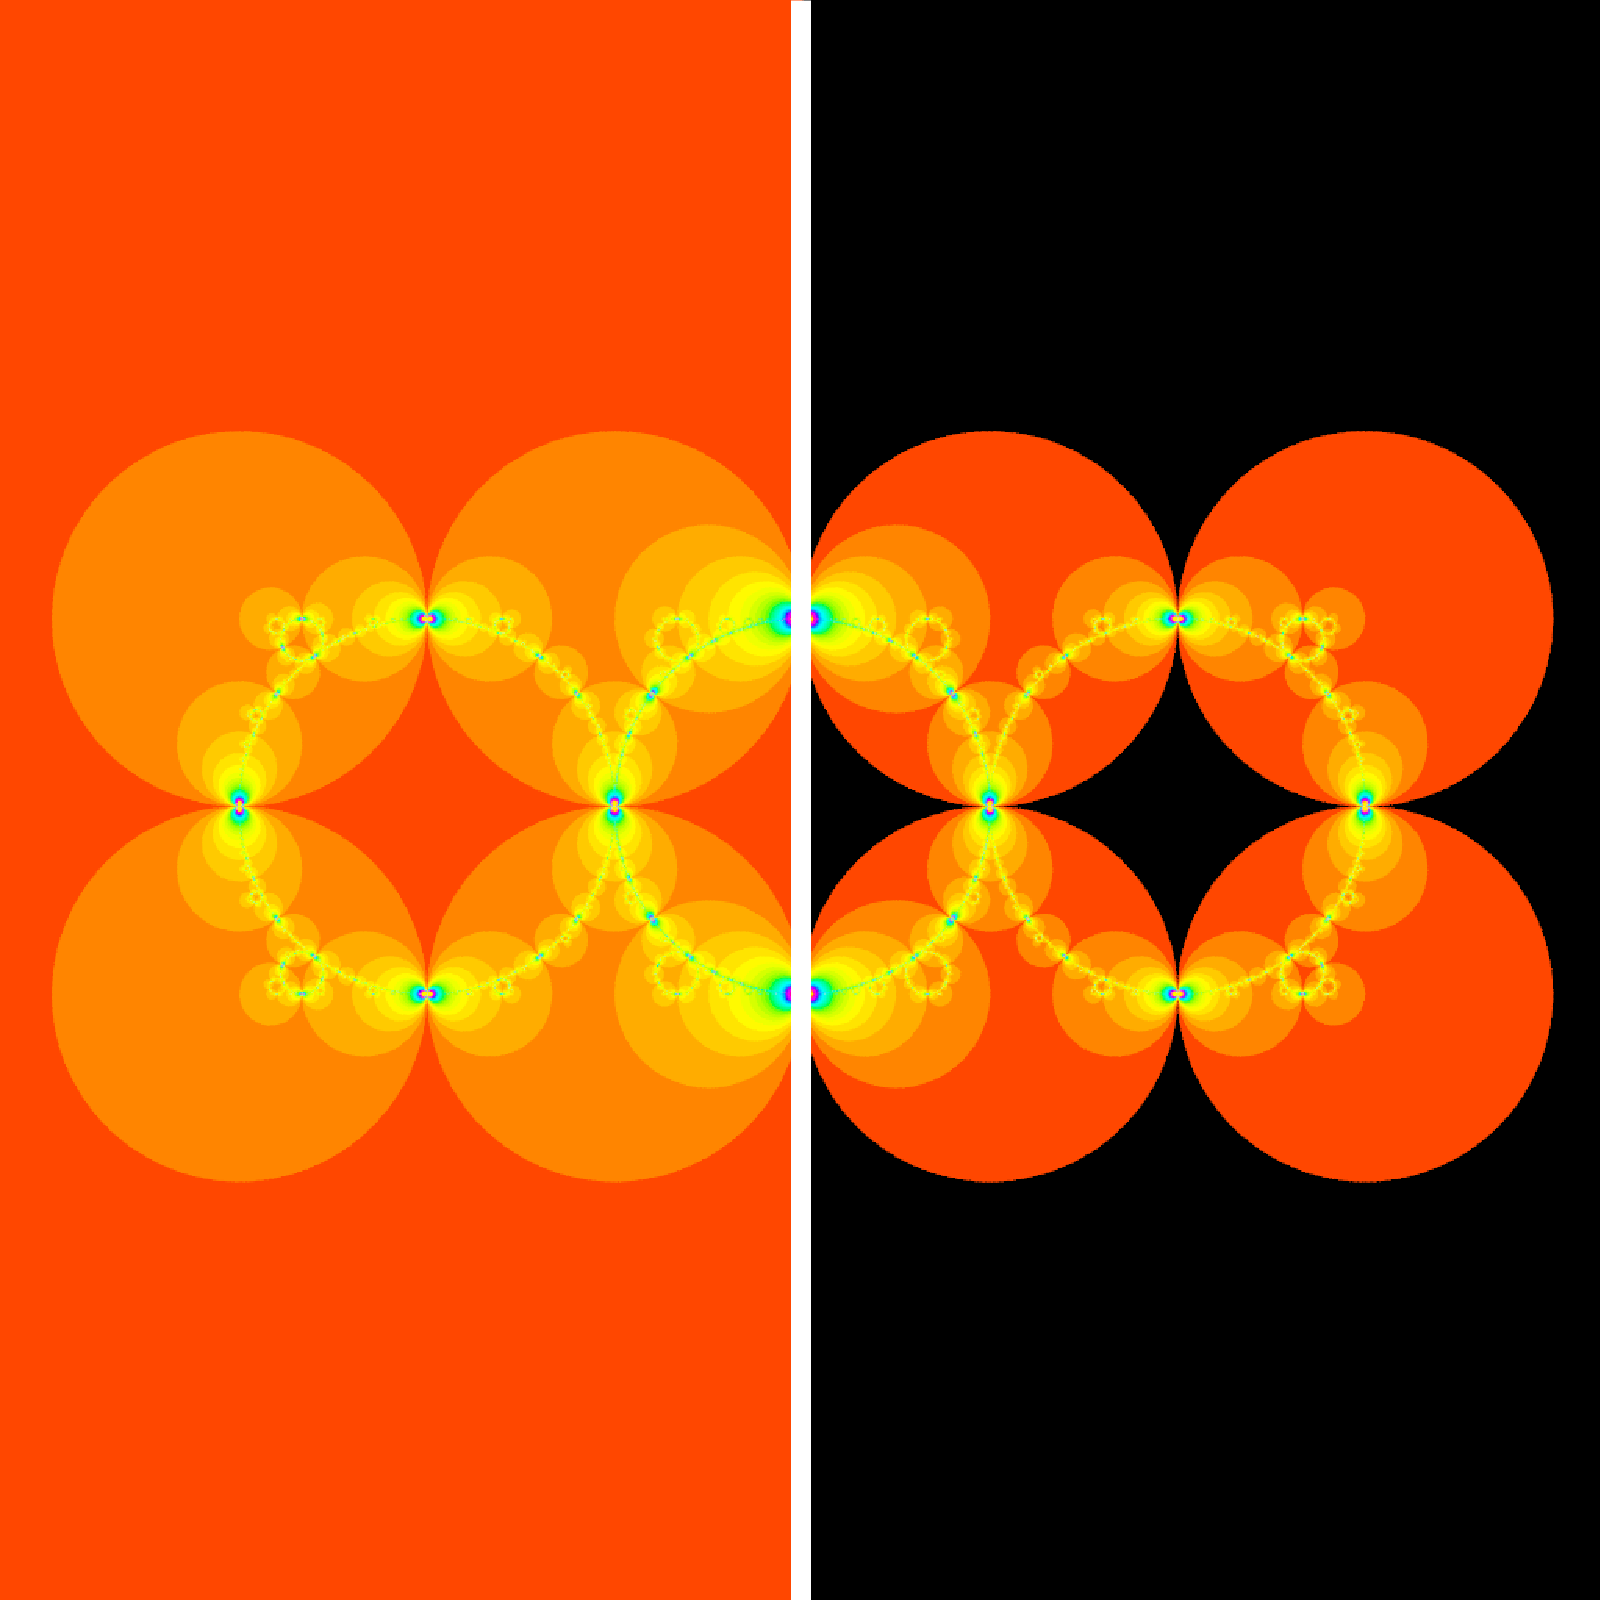
\includegraphics[ height=1.4in, keepaspectratio]{./img/application/2dGen/infInvEdgedOrb.pdf}
   \subcaption{\textit{Orbit}}
   \label{fig:infCircleOrb}
  \end{minipage}
  \hspace*{\fill}
  \caption{\textit{Inversion in the circle with \\ infinite radius and
  four Schottky disks}}
  \label{fig:infCircle}
 \end{minipage}
 \begin{minipage}[t]{0.5\hsize}
  \begin{minipage}{0.25\hsize}
   \center
   
\includegraphics[ height=1.4in, keepaspectratio]{./img/application/2dGen/translationEdgedGen.pdf}
   \subcaption{\textit{Generator}}
   \label{fig:translation2dGen}
  \end{minipage}
  \hspace*{\fill}
  \begin{minipage}{0.25\hsize}
   \center
   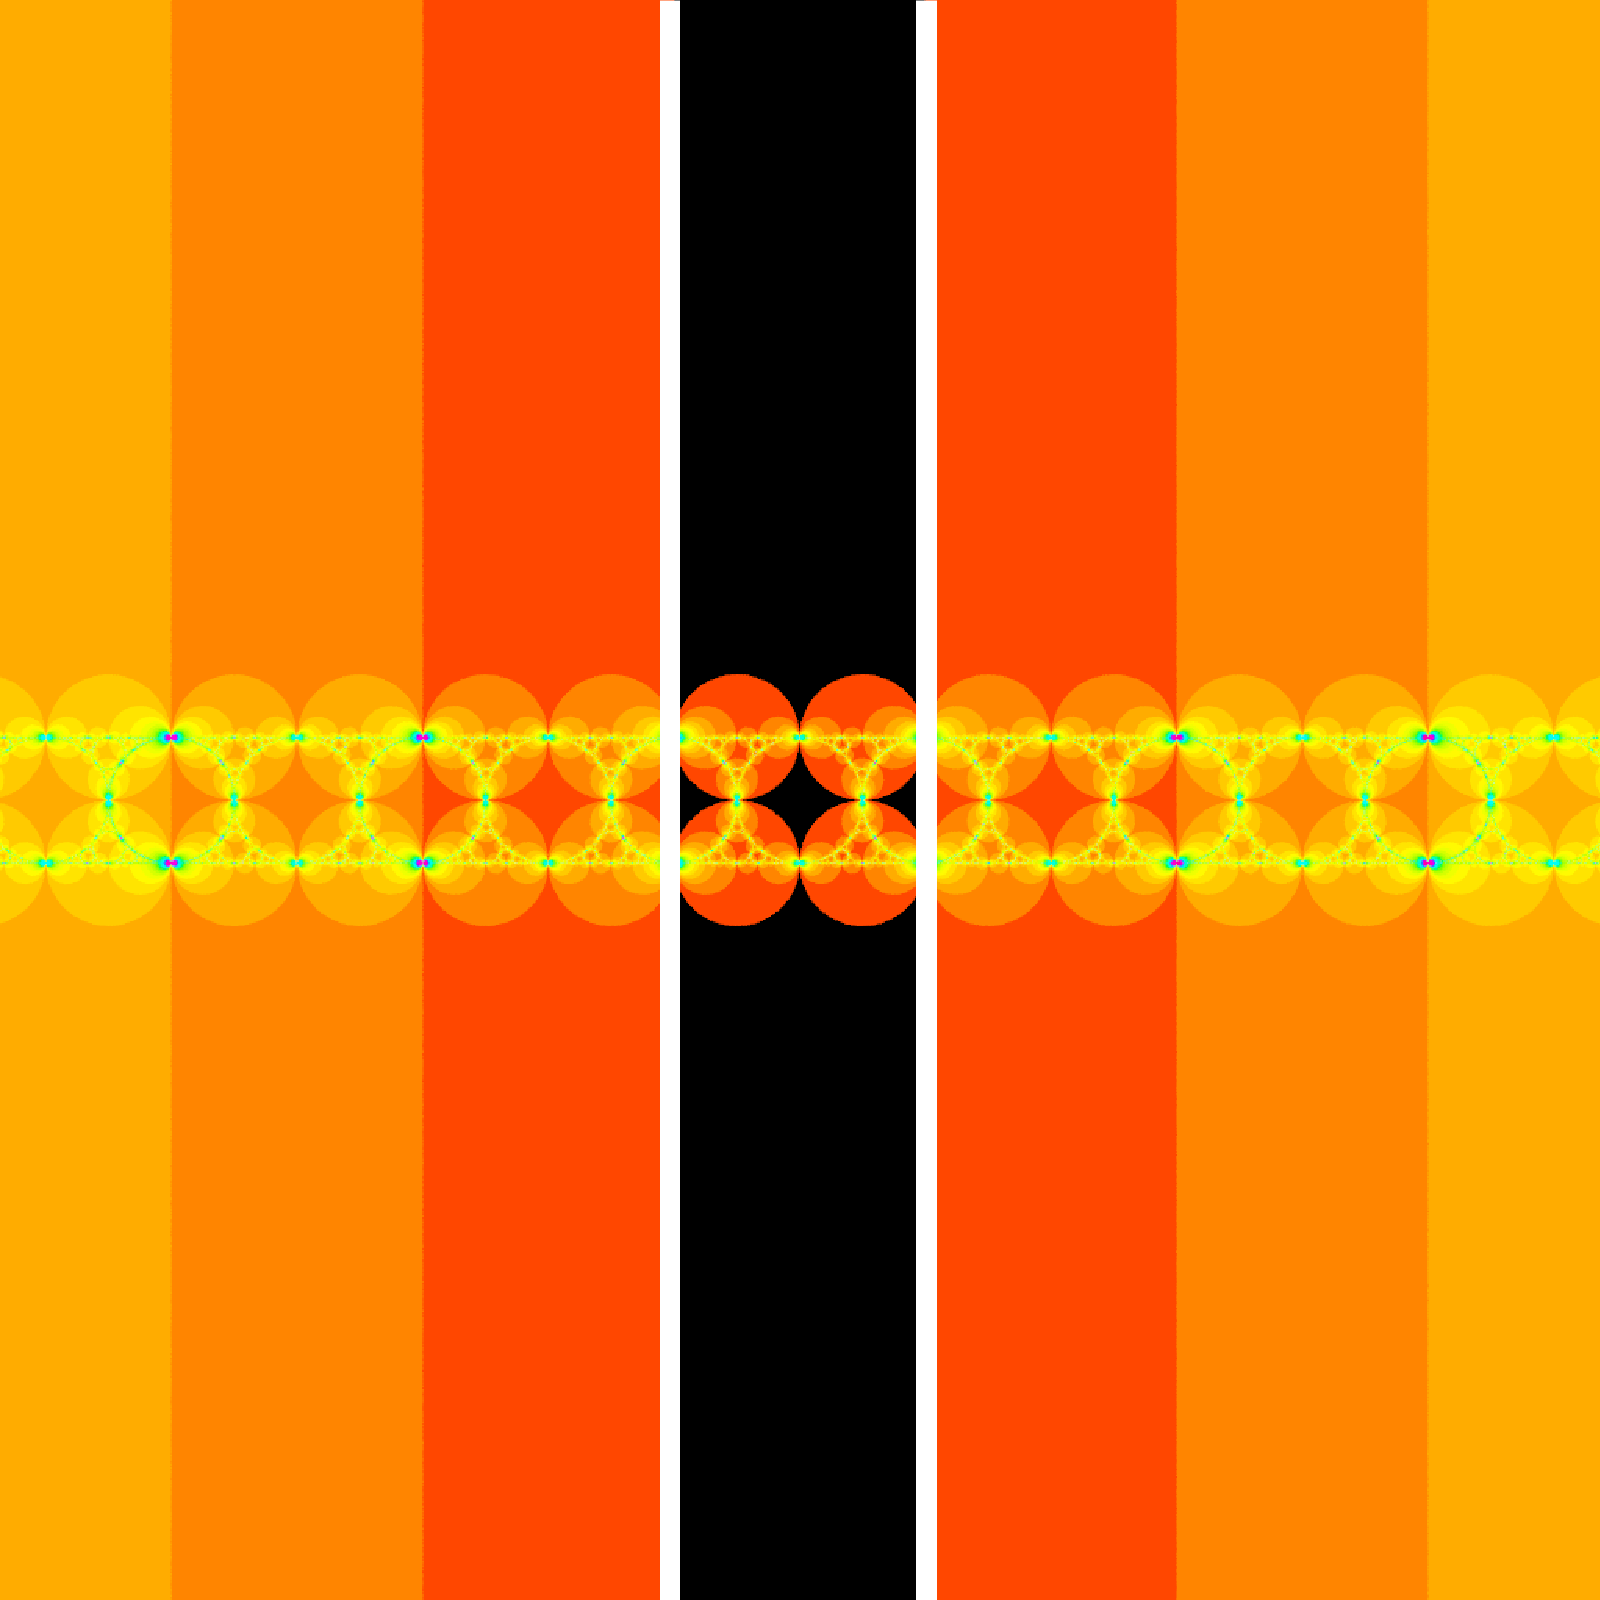
\includegraphics[ height=1.4in, keepaspectratio]{./img/application/2dGen/translationEdgedOrb.pdf}
   \subcaption{\textit{Orbit}}
   \label{fig:translation2dOrb}
  \end{minipage}
  \hspace*{\fill}
  \caption{\textit{Parallel translation generator and four Schottky disks}}
  \label{fig:translation2d}
 \end{minipage}
 \end{figure}

\begin{figure}[htbp]
 \begin{minipage}{0.5\hsize}
  \begin{minipage}{0.25\hsize}
   \center
   
\includegraphics[ height=1.4in, keepaspectratio]{./img/application/2dGen/rotationEdgedGen.pdf}
   \subcaption{\textit{Generator}}
   \label{fig:rotation2dGen}
  \end{minipage}
 \hspace*{\fill}
  \begin{minipage}{0.25\hsize}
   \center
   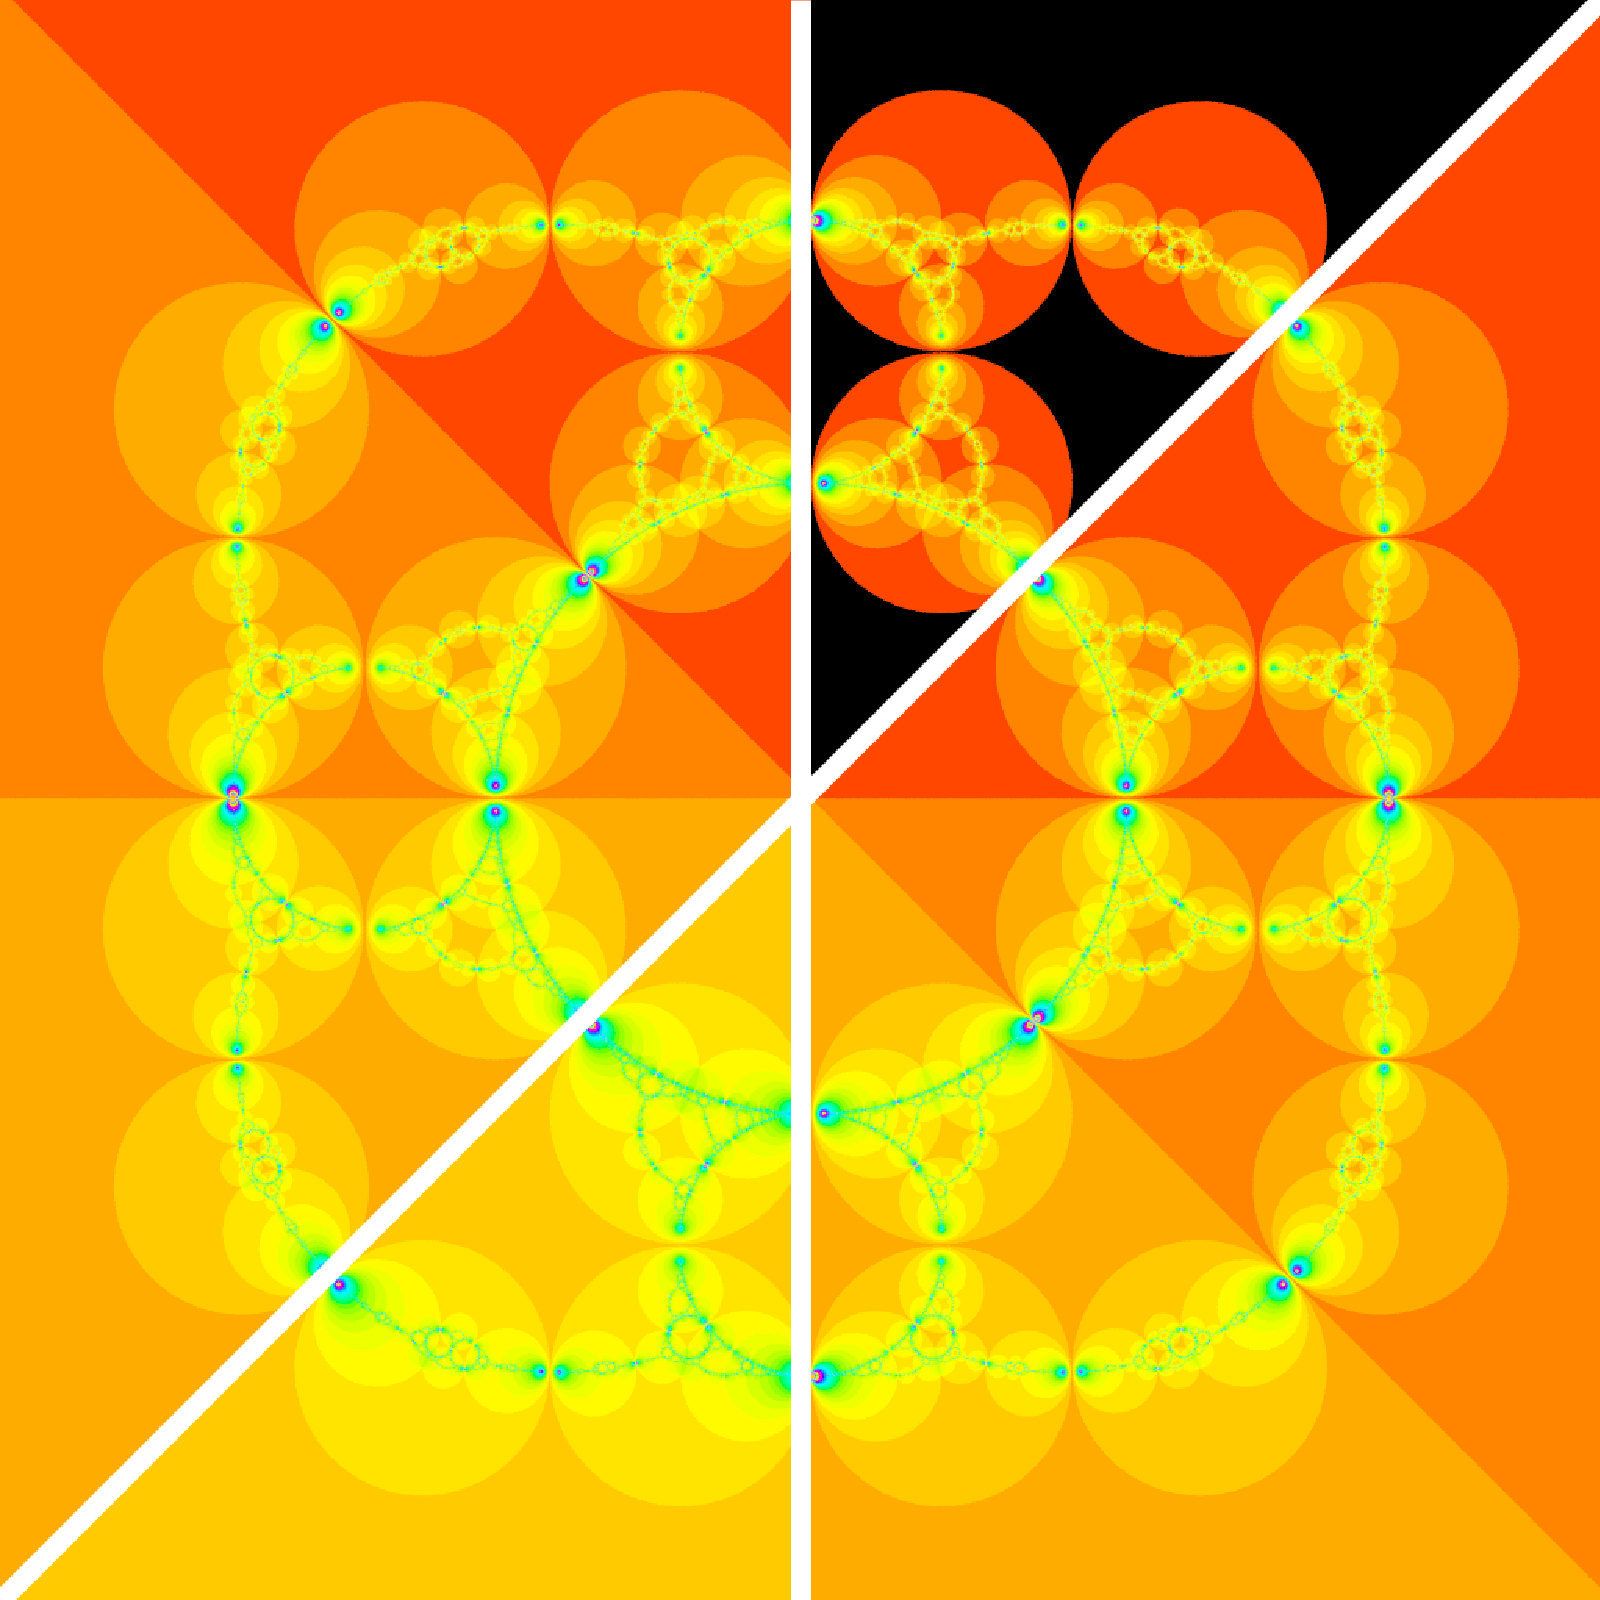
\includegraphics[ height=1.4in, keepaspectratio]{./img/application/2dGen/rotationEdgedOrb.pdf}
   \subcaption{\textit{Orbit}}
   \label{fig:rotation2dOrb}
  \end{minipage}
  \hspace*{\fill}
  \caption{\textit{Rotation generator and three Schottky disks}}
  \label{fig:rotation2d}
 \end{minipage}
 \begin{minipage}{0.5\hsize}
  \begin{minipage}{0.25\hsize}
   \center
   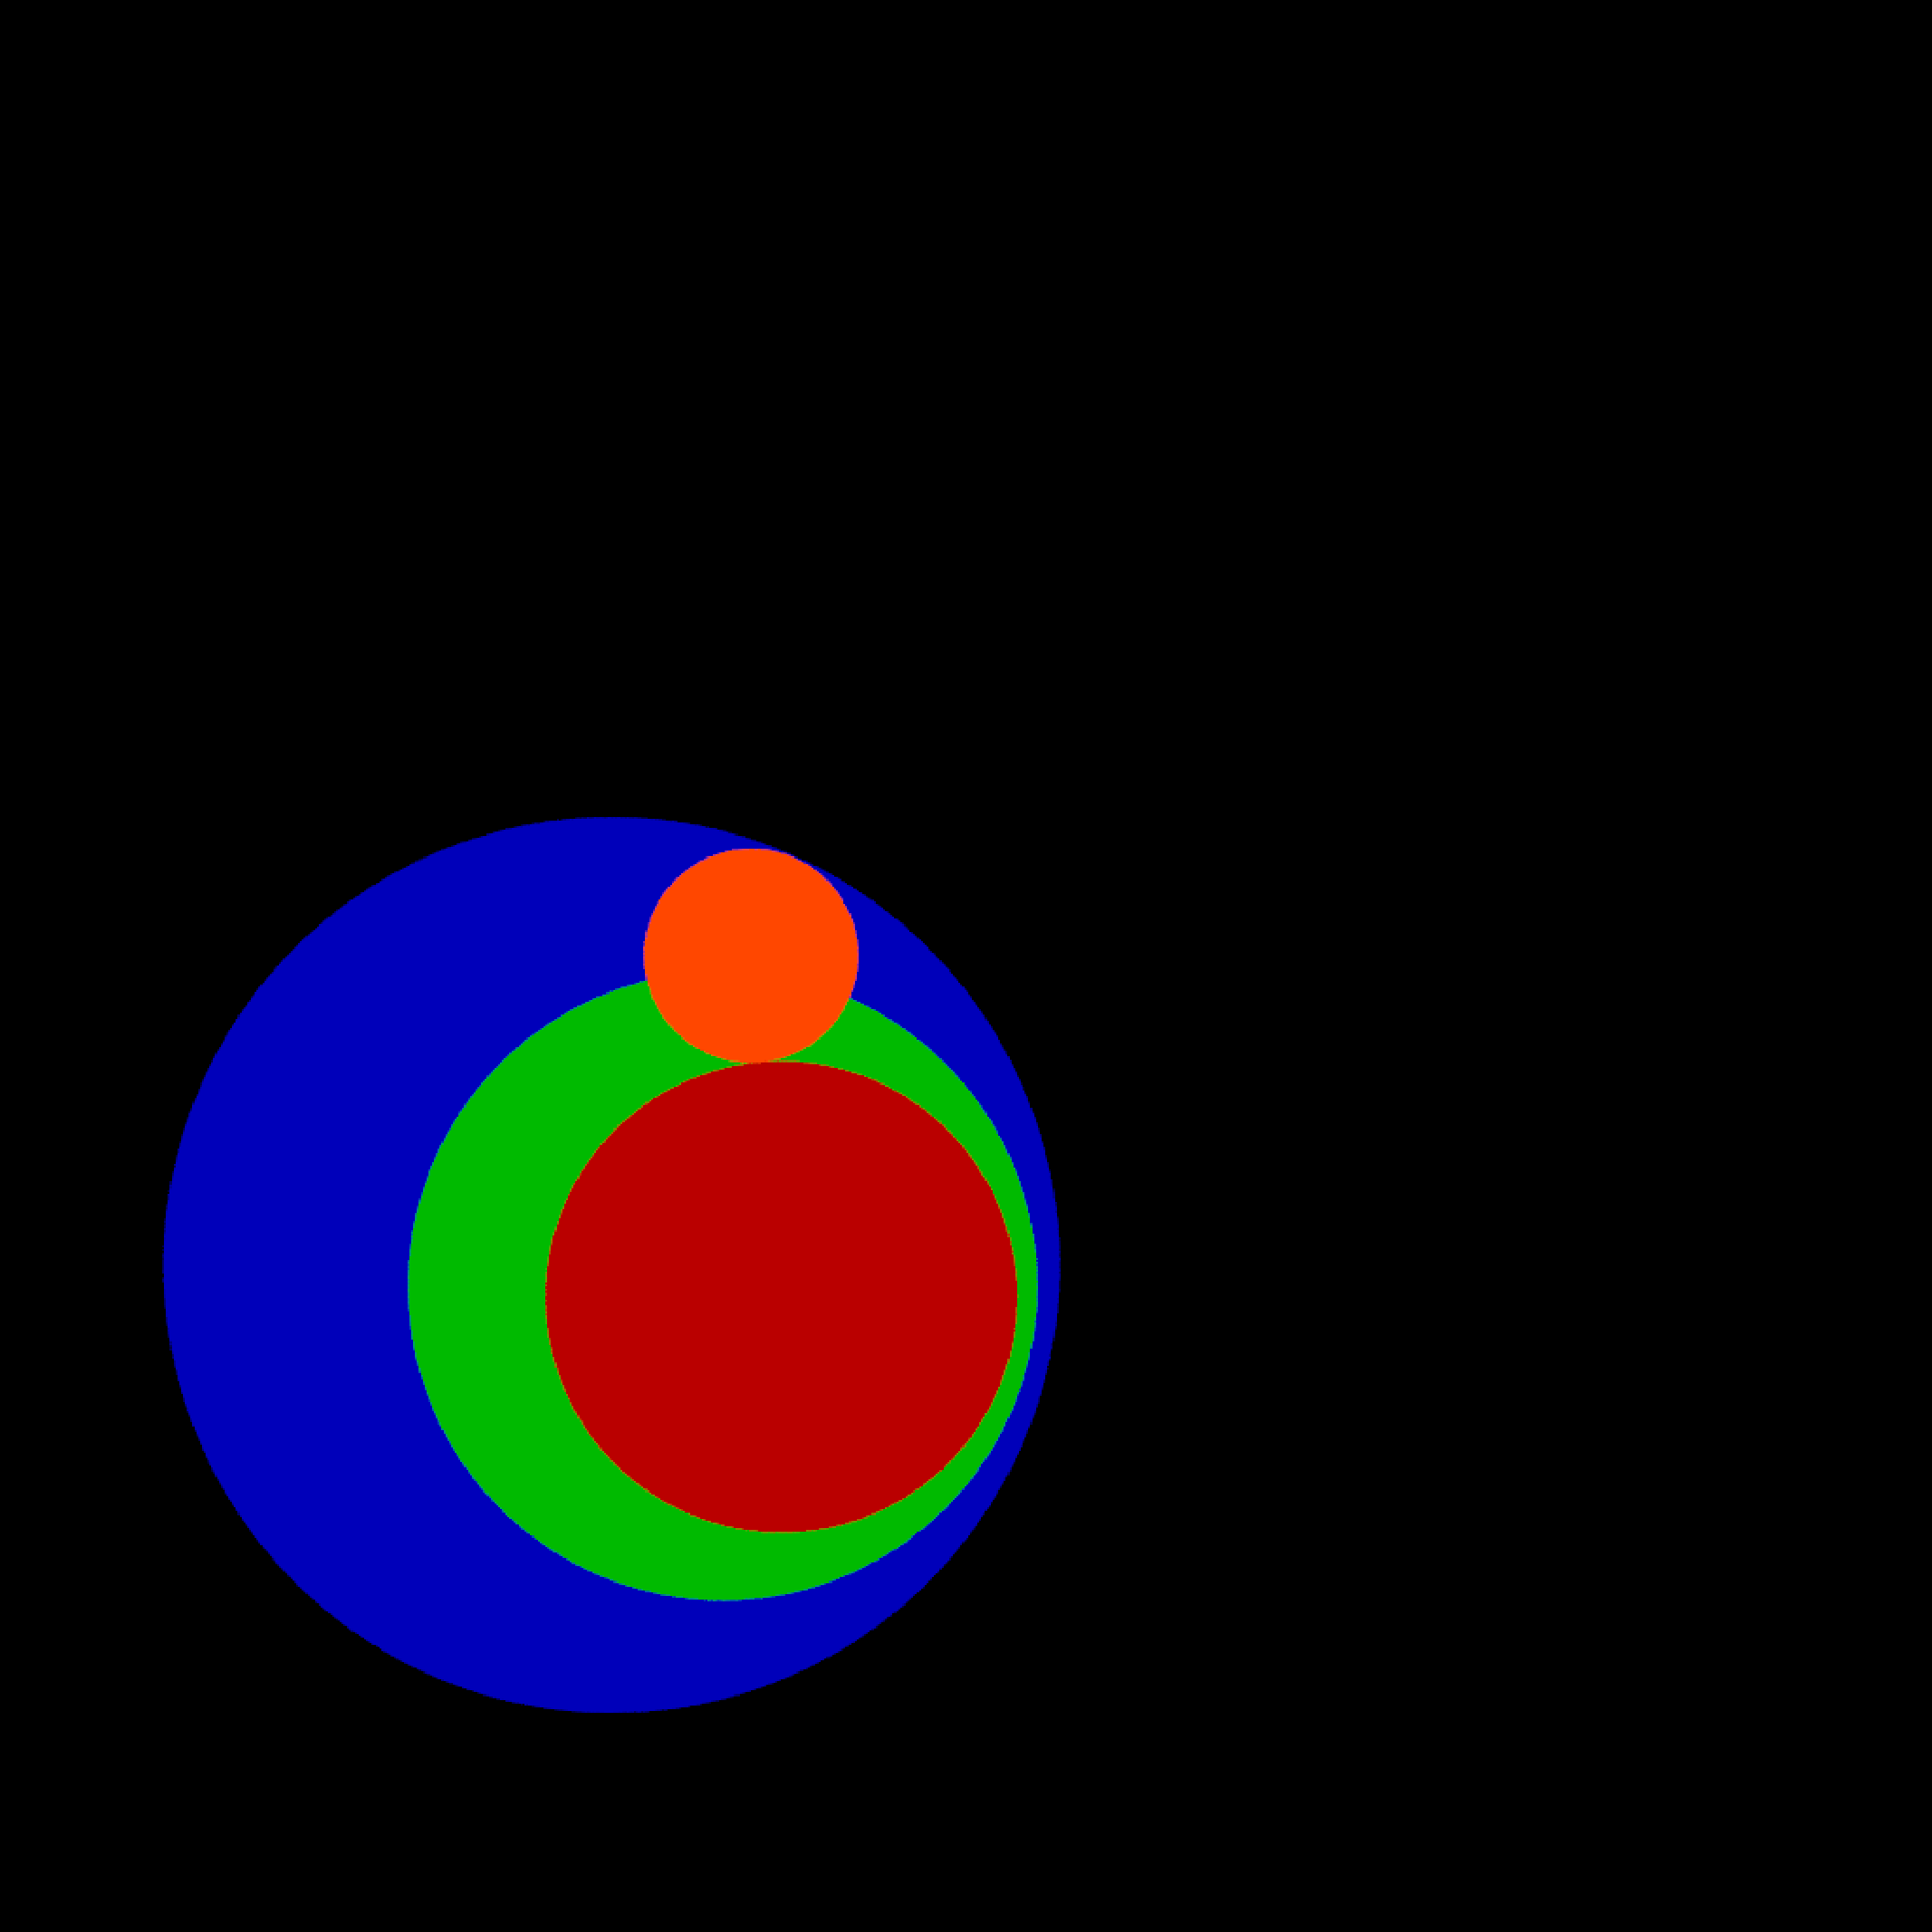
\includegraphics[ height=1.4in, keepaspectratio]{./img/application/2dGen/hyperbolicRect0.pdf}
   \subcaption{\textit{Generator}}
   \label{fig:hyperbolic2dGen}
  \end{minipage}
 \hspace*{\fill}
  \begin{minipage}{0.25\hsize}
   \center
   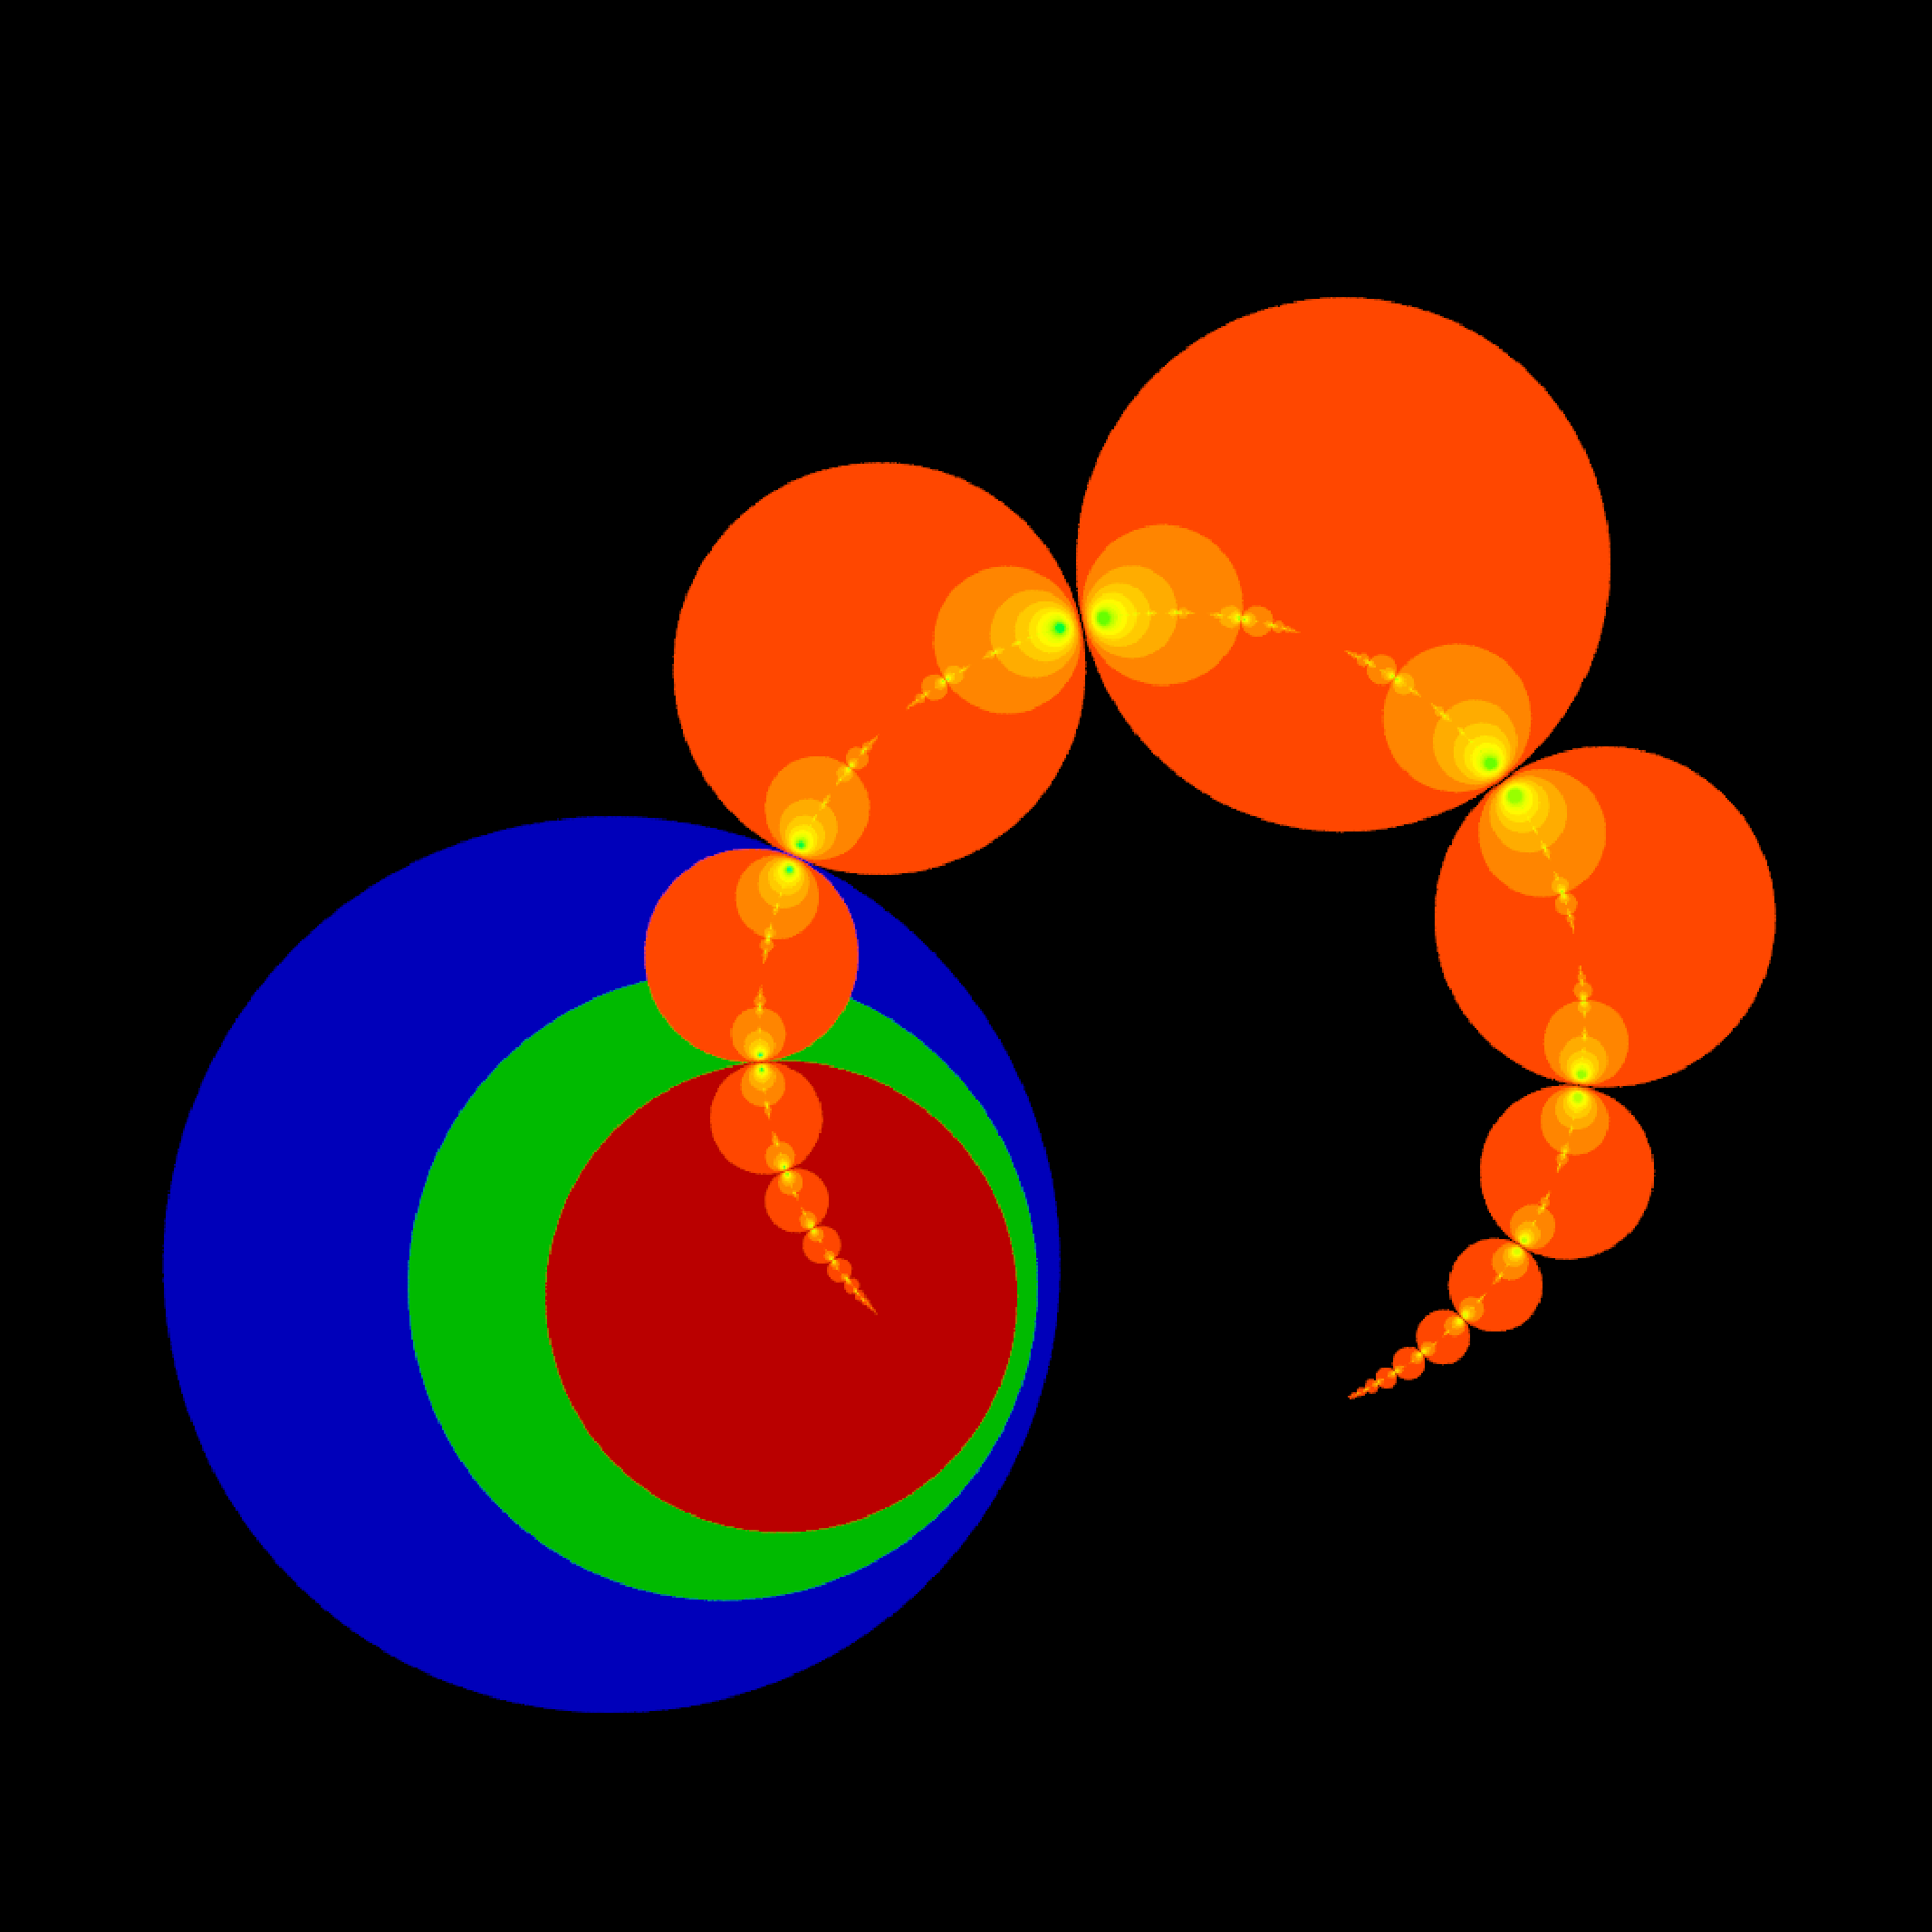
\includegraphics[ height=1.4in, keepaspectratio]{./img/application/2dGen/hyperbolicRect.pdf}
   \subcaption{\textit{Orbit}}
   \label{fig:hyperbolic2dOrb}
  \end{minipage}
 \hspace*{\fill}
  \caption{\textit{Hyperbolic generator and a Schottky disk}}
  \label{fig:hyperbolic2d}
 \end{minipage}
\end{figure}

\begin{figure}[htbp]
 \begin{minipage}[t]{0.5\hsize}
  \begin{minipage}{0.25\hsize}
   \center
   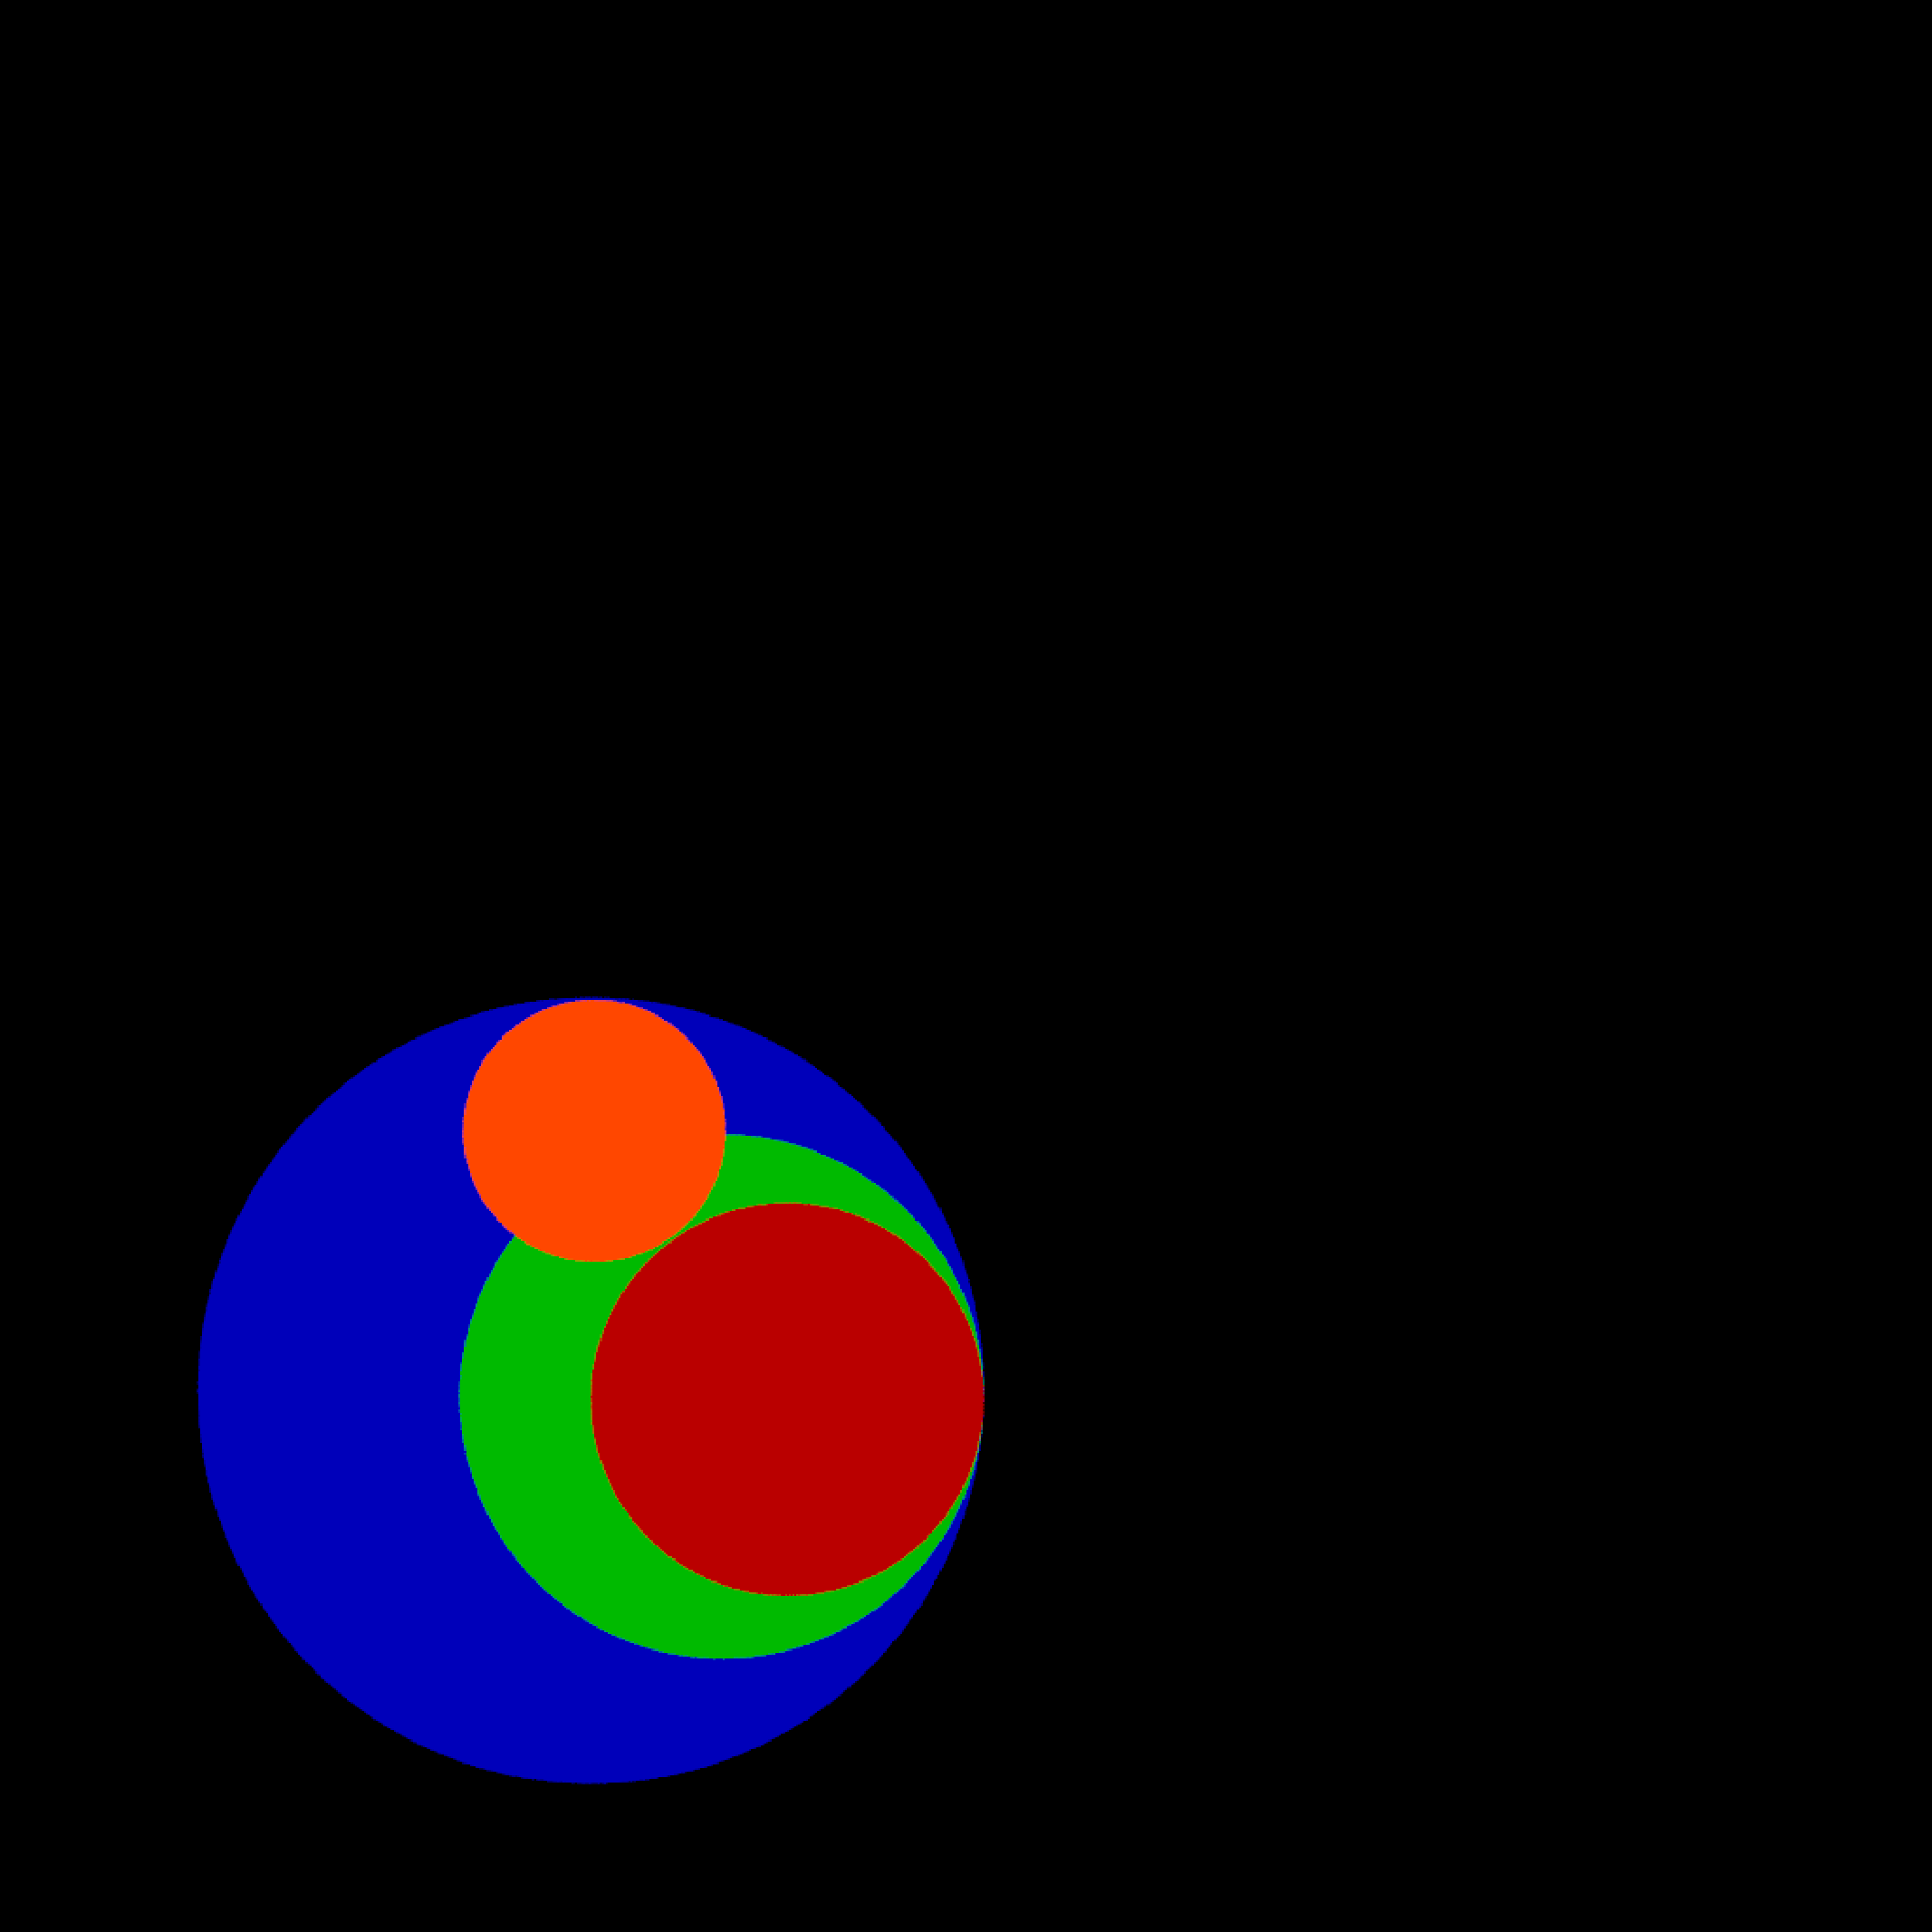
\includegraphics[ height=1.4in, keepaspectratio]{./img/application/2dGen/parabolicRect0.pdf}
   \subcaption{\textit{Generator}}
   \label{fig:parabolic2dGen}
  \end{minipage}
 \hspace*{\fill}
  \begin{minipage}{0.25\hsize}
   \center
   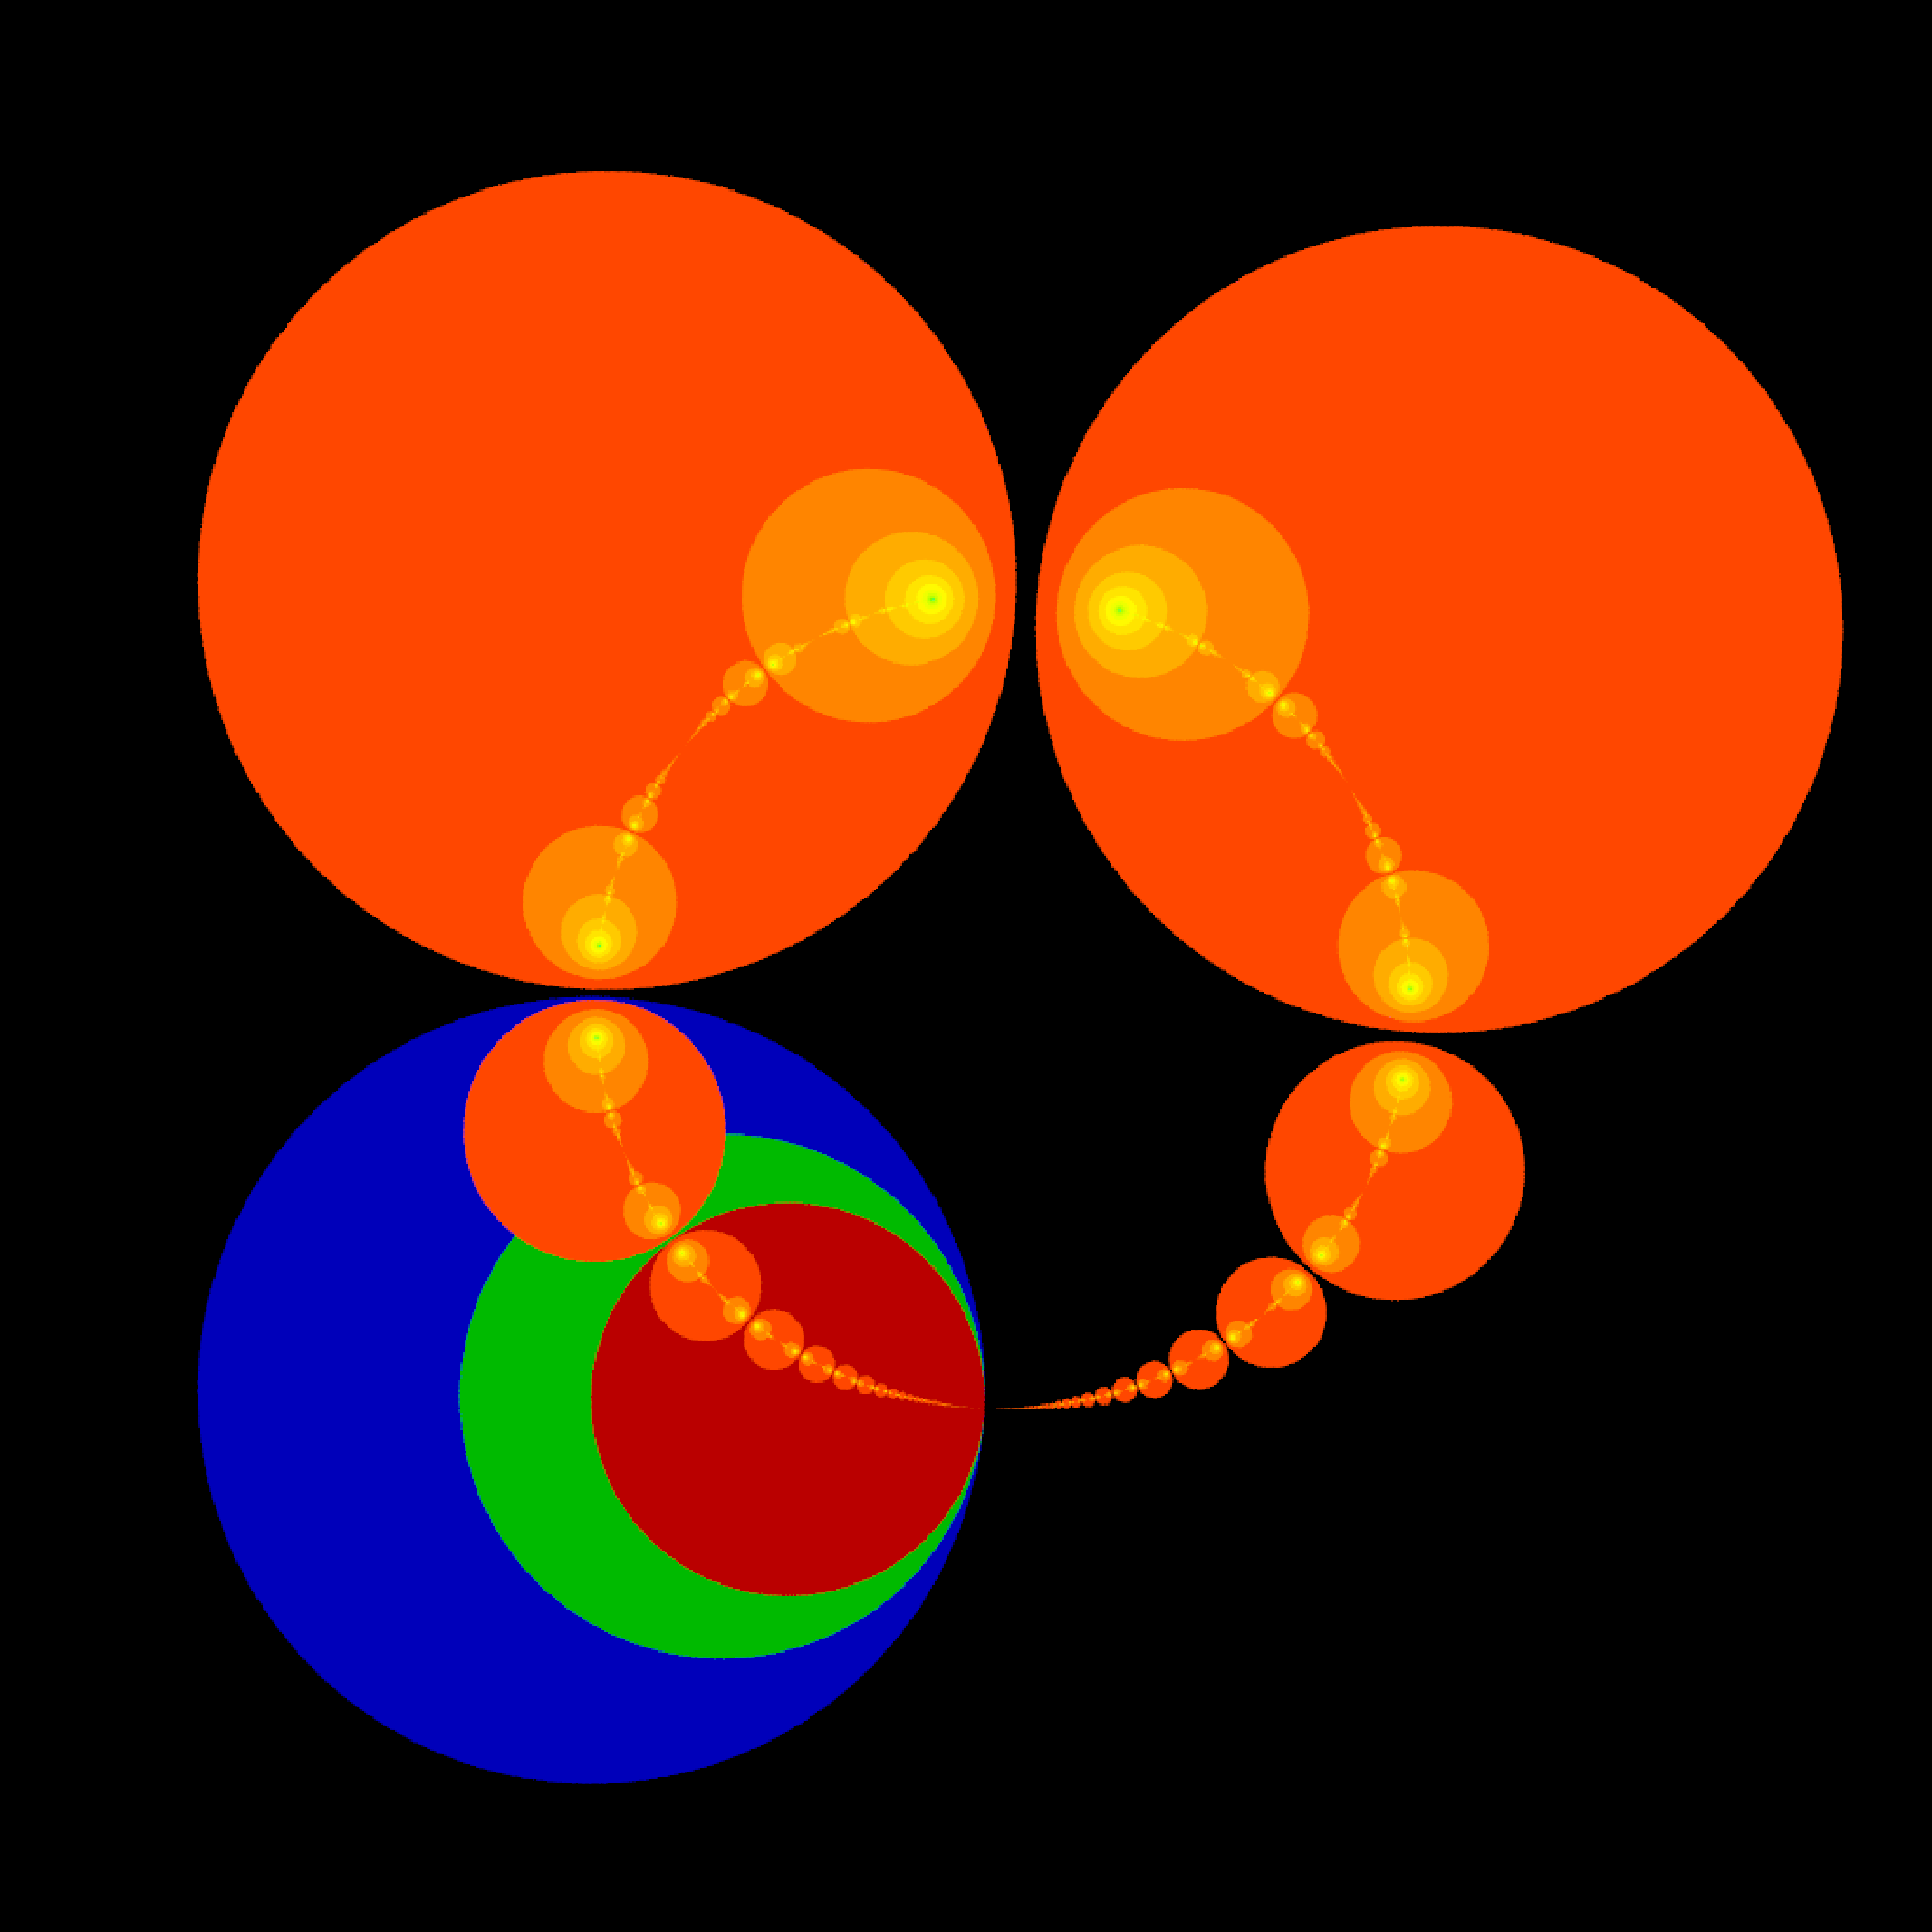
\includegraphics[ height=1.4in, keepaspectratio]{./img/application/2dGen/parabolicRect.pdf}
   \subcaption{\textit{Orbit}}
   \label{fig:parabolic2dOrb}
  \end{minipage}
  \hspace*{\fill}
  \caption{\textit{The orbit of Parabolic generator and \\a Schottky disk}}
  \label{fig:parabolic2d}
 \end{minipage}
 \begin{minipage}[t]{0.5\hsize}
  \begin{minipage}{0.25\hsize}
   \center
   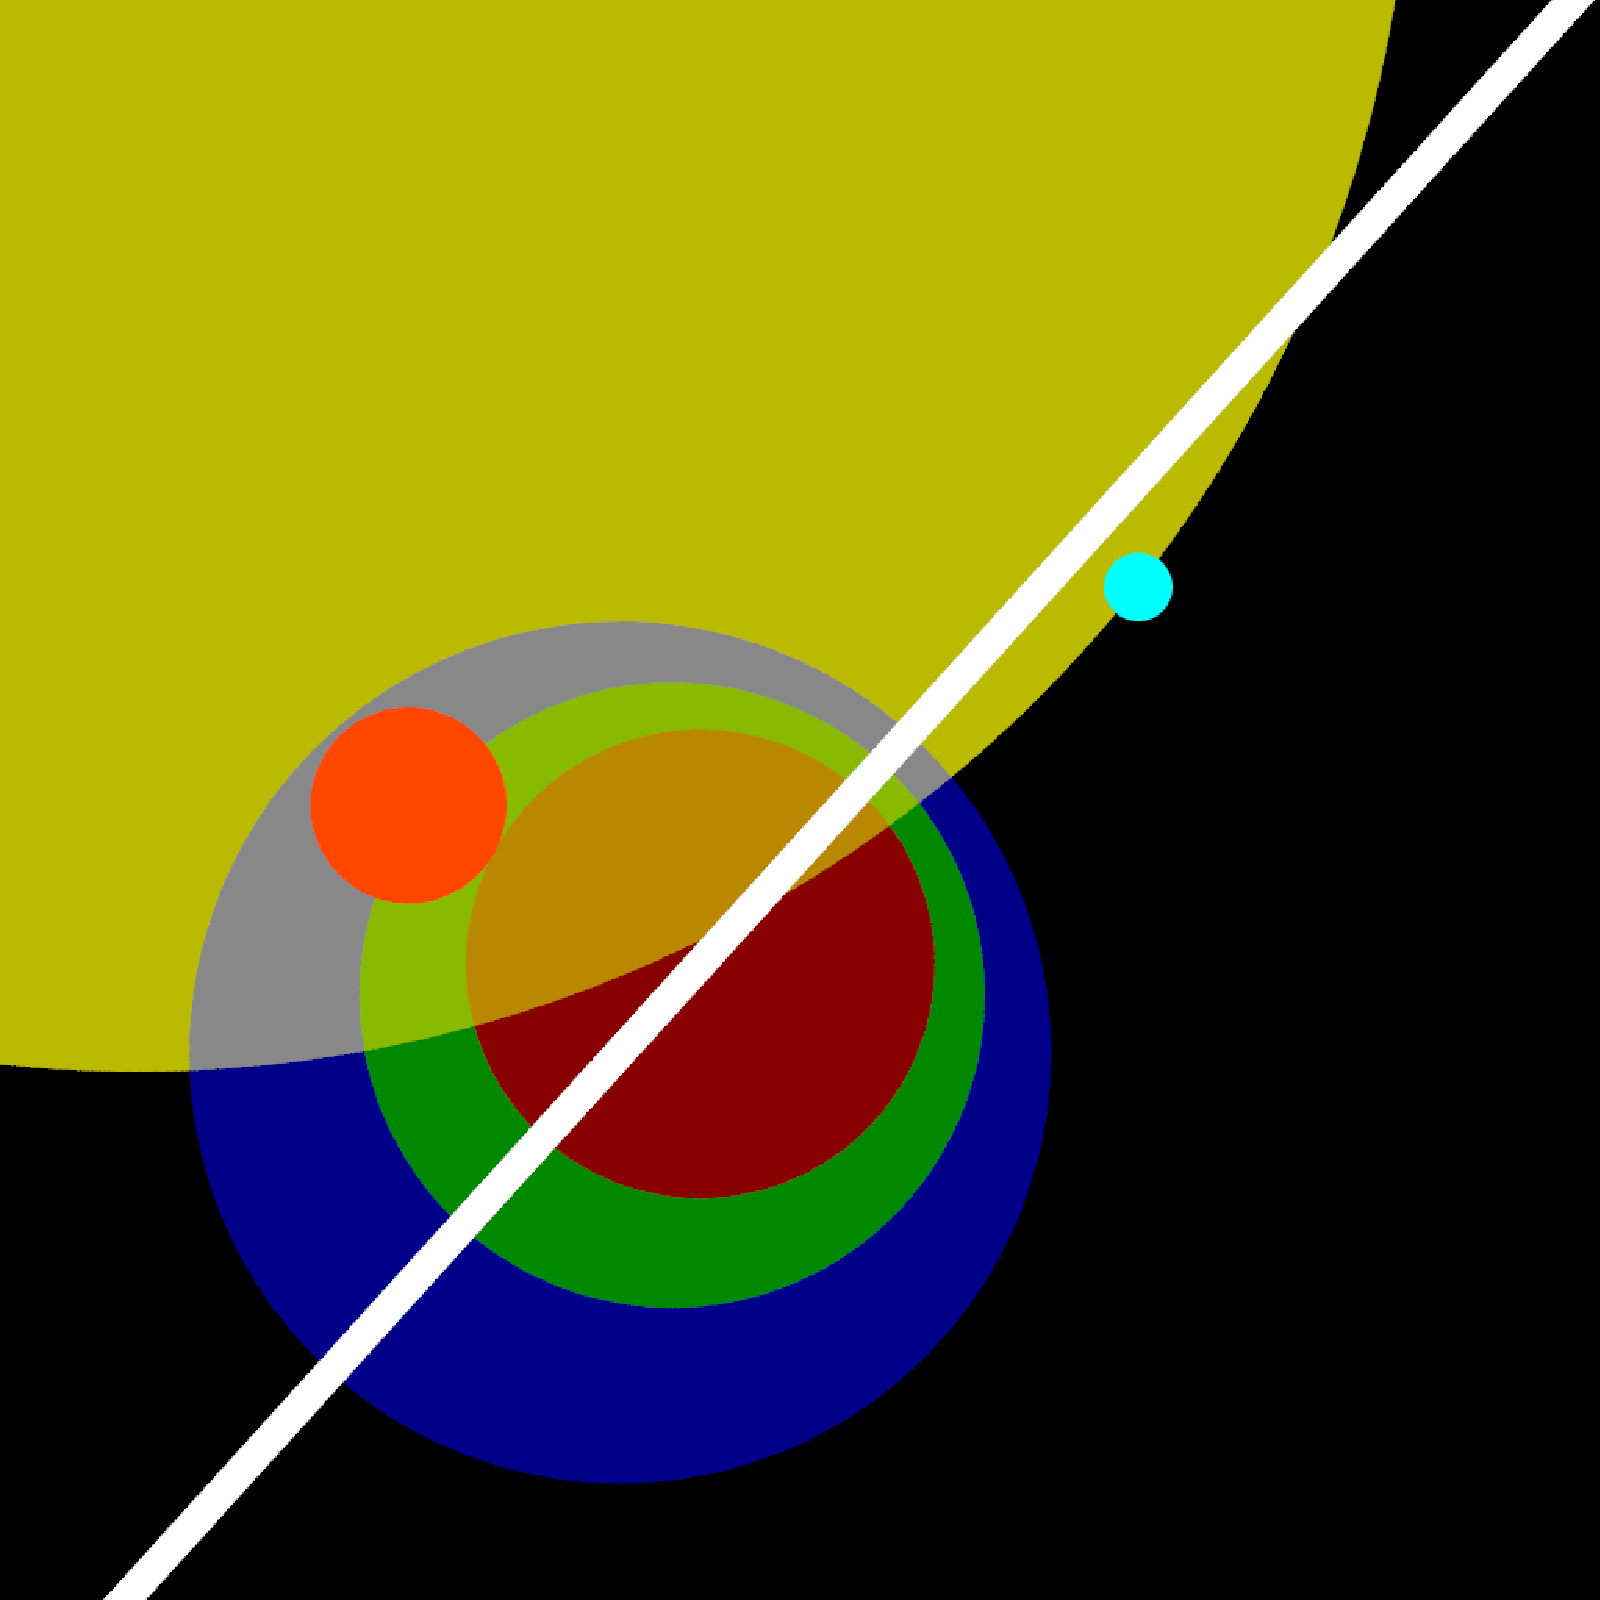
\includegraphics[ height=1.4in, keepaspectratio]{./img/application/2dGen/loxo0.pdf}
   \subcaption{\textit{Generator}}
   \label{fig:loxo2dGen}
  \end{minipage}
 \hspace*{\fill}
  \begin{minipage}{0.25\hsize}
   \center
   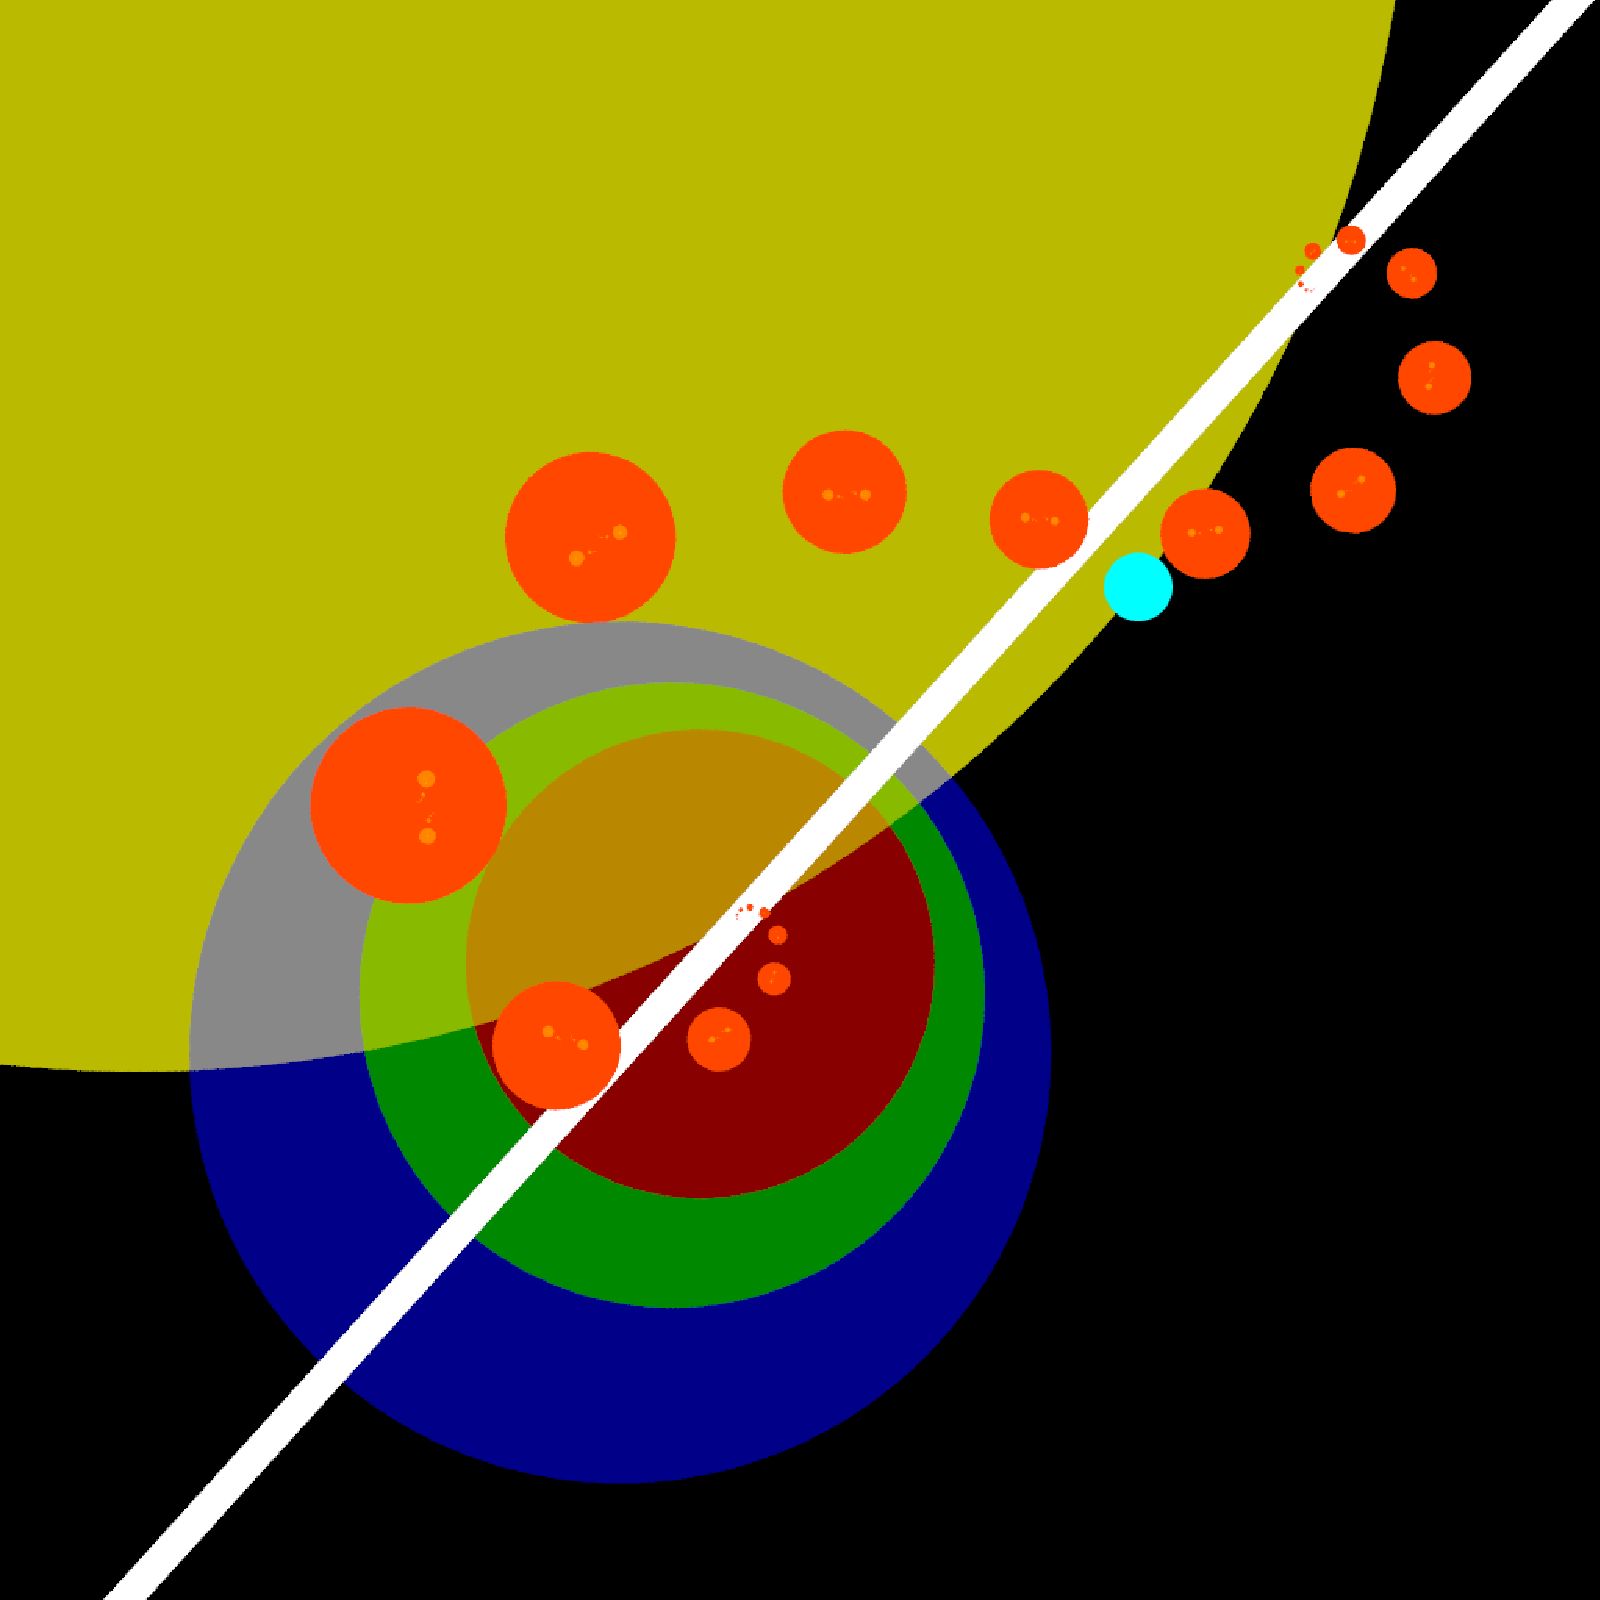
\includegraphics[ height=1.4in, keepaspectratio]{./img/application/2dGen/loxoOrb.pdf}
   \subcaption{\textit{Orbit}}
   \label{fig:loxo2dOrb}
  \end{minipage}
 \hspace*{\fill}
  \caption{\textit{Loxodromic generator and a Schottky disk}}
  \label{fig:loxodromic2d}
 \end{minipage}
\end{figure}

\noindent\textbf{Inversion in a Circle with Infinite Radius.}
An inversion in a circle with infinite radius is treated as a reflection
over a border line of half plane. See Figure
\ref{fig:infCircle}\subref{fig:infCircleGen}.
The four inversion circles are lying on the right side, and there is the
orange region on the left side. The region is is a half plane, that is, a
disk with infinite radius. Its boundary is colored with white line.
The orbit is shown in
Figure \ref{fig:infCircle}\subref{fig:infCircleOrb}.
As we can see, the circles are reflected over the white line.

\noindent\textbf{Parallel Translation.}
A composition of reflections over two parallel half planes facing each
other generates a parallel translation. See Figure
\ref{fig:translation2d}\subref{fig:translation2dGen}.
There are two orange half planes on the right and left sides.
The orbit is shown in Figure
\ref{fig:translation2d}\subref{fig:translation2dOrb}.

\noindent\textbf{Rotation.}
A composition of reflections over two crossing half planes generates a
rotation. The generator is shown in Figure
\ref{fig:rotation2d}\subref{fig:rotation2dGen}
The two half planes are crossing. The rotation axis is crossing point of
white border lines. The orbit is shown in Figure 
\ref{fig:rotation2d}\subref{fig:rotation2dOrb}.
It has a rotation symmetry and it is an elliptic transformation.

\noindent\textbf{Composition of Two Circles.}
 Next, we use a composition of inversions in two circles.
 See Figure \ref{fig:hyperbolic2d}\subref{fig:hyperbolic2dGen}.
 There are one Schottky disk and three regions colored with red, green,
 and blue.
 We call the boundary of red disk $C1$, 
 the outer circle of green region $C2$, and
 let $C1'$ be the inversion of $C1$ in $C2$.
 The outer circle of blue region is $C1'$.
 The generator is composed of $C1$, $C2$, and $C1'$.
 While $C1$ and $C2$ have no intersection, the composition of inversions
 in $C1$ and $C2$ represents hyperbolic transformations
 \footnote{\url{https://www.shadertoy.com/view/MsScWW}}.
 The orbit is shown in Figure
 \ref{fig:hyperbolic2d}\subref{fig:hyperbolic2dOrb}.
 The orbit of the disk converges to two fixed points.
 We compose the map $G$ as follows.
 The prefix $I$ represents an inversion, for example, $I_{C1}$ represents
 an inversion in $C1$.
 \begin{align*}
  G =
  \begin{cases}
   I_{C2} \circ I_{C1} & (\text{The point is inside of } C1) \\
   I_{C1} \circ I_{C2} & (\text{The point is outside of }C1')
  \end{cases}
 \end{align*}
 In the process of IIS, we can transform the point to the fundamental
 domain by applying $G$ repeatedly.
 The fundamental domain of this type of generators is the blue and green
 area in Figure \ref{fig:hyperbolic2d}\subref{fig:hyperbolic2dGen}..

 Then, we displace $C1$.
 When $C1$ and $C2$ are kissing as shown in Figure 
 \ref{fig:parabolic2d}\subref{fig:parabolic2dGen},
 this generator becomes a parabolic transformation
 \footnote{\url{https://www.shadertoy.com/view/XsBcDD}}.
 The fixed points overlap each other, and the orbit converges to the
 point as shown in Figure \ref{fig:parabolic2d}\subref{fig:parabolic2dOrb}.

 When $C1$ and $C2$ are crossing as in Figure n, 
 the generator becomes an elliptic transformation.
 The orbit is as shown in Figure n.
 The disks are rotate around crossing line.
 Note that crossing angle of $C1$ and $C2$ should be rational angles,
 otherwise the orbit of the disks will overlap each other.

\noindent\textbf{Loxodromic.}
 We can twist the orbit by adding another two inversions.
 See Figure \ref{fig:loxodromic2d}\subref{fig:loxo2dGen}.
 The yellow disk and the white line are added to the hyperbolic generator.
 The white line is a line with two centers of $C1$ and $C2$.
 We call the line $L$, the boundary of the yellow disk $C3$, and
 light blue point $P$.
 $P$ is a user-defined control point, and the circle $C3$ is determined
 by three points, one is the point $P$, and the others are inversions
 of $P$ in $C1$ and $C2$.
 $L$ and $C3$ are perpendicular to $C1$ and $C2$.
 Thus, a composition of the reflection over $L$ and the inversion in $C3$
 represents a rotation, and
 the orbit of the group is twisted as shown in Figure
 \ref{fig:loxodromic2d}\subref{fig:loxo2dOrb}. This is a loxodromic
 transformation\footnote{\url{https://www.shadertoy.com/view/lsSyDW}}.
 The map $G$ is as follows.
 \begin{align*}
  G =
  \begin{cases}
   (I_{C2} \circ I_{C1}) \circ (I_{C3} \circ I_L) & (\text{The point is inside of } C1) \\
   (I_L \circ I_{C3}) \circ (I_{C1} \circ I_{C2}) & (\text{The point is outside of }C1')
  \end{cases}
 \end{align*}

\subsubsection{Three Dimensionanl Generators}

\begin{figure}[h!tbp]
 \begin{minipage}[t]{0.5\hsize}
  \begin{minipage}{0.25\hsize}
   \center
   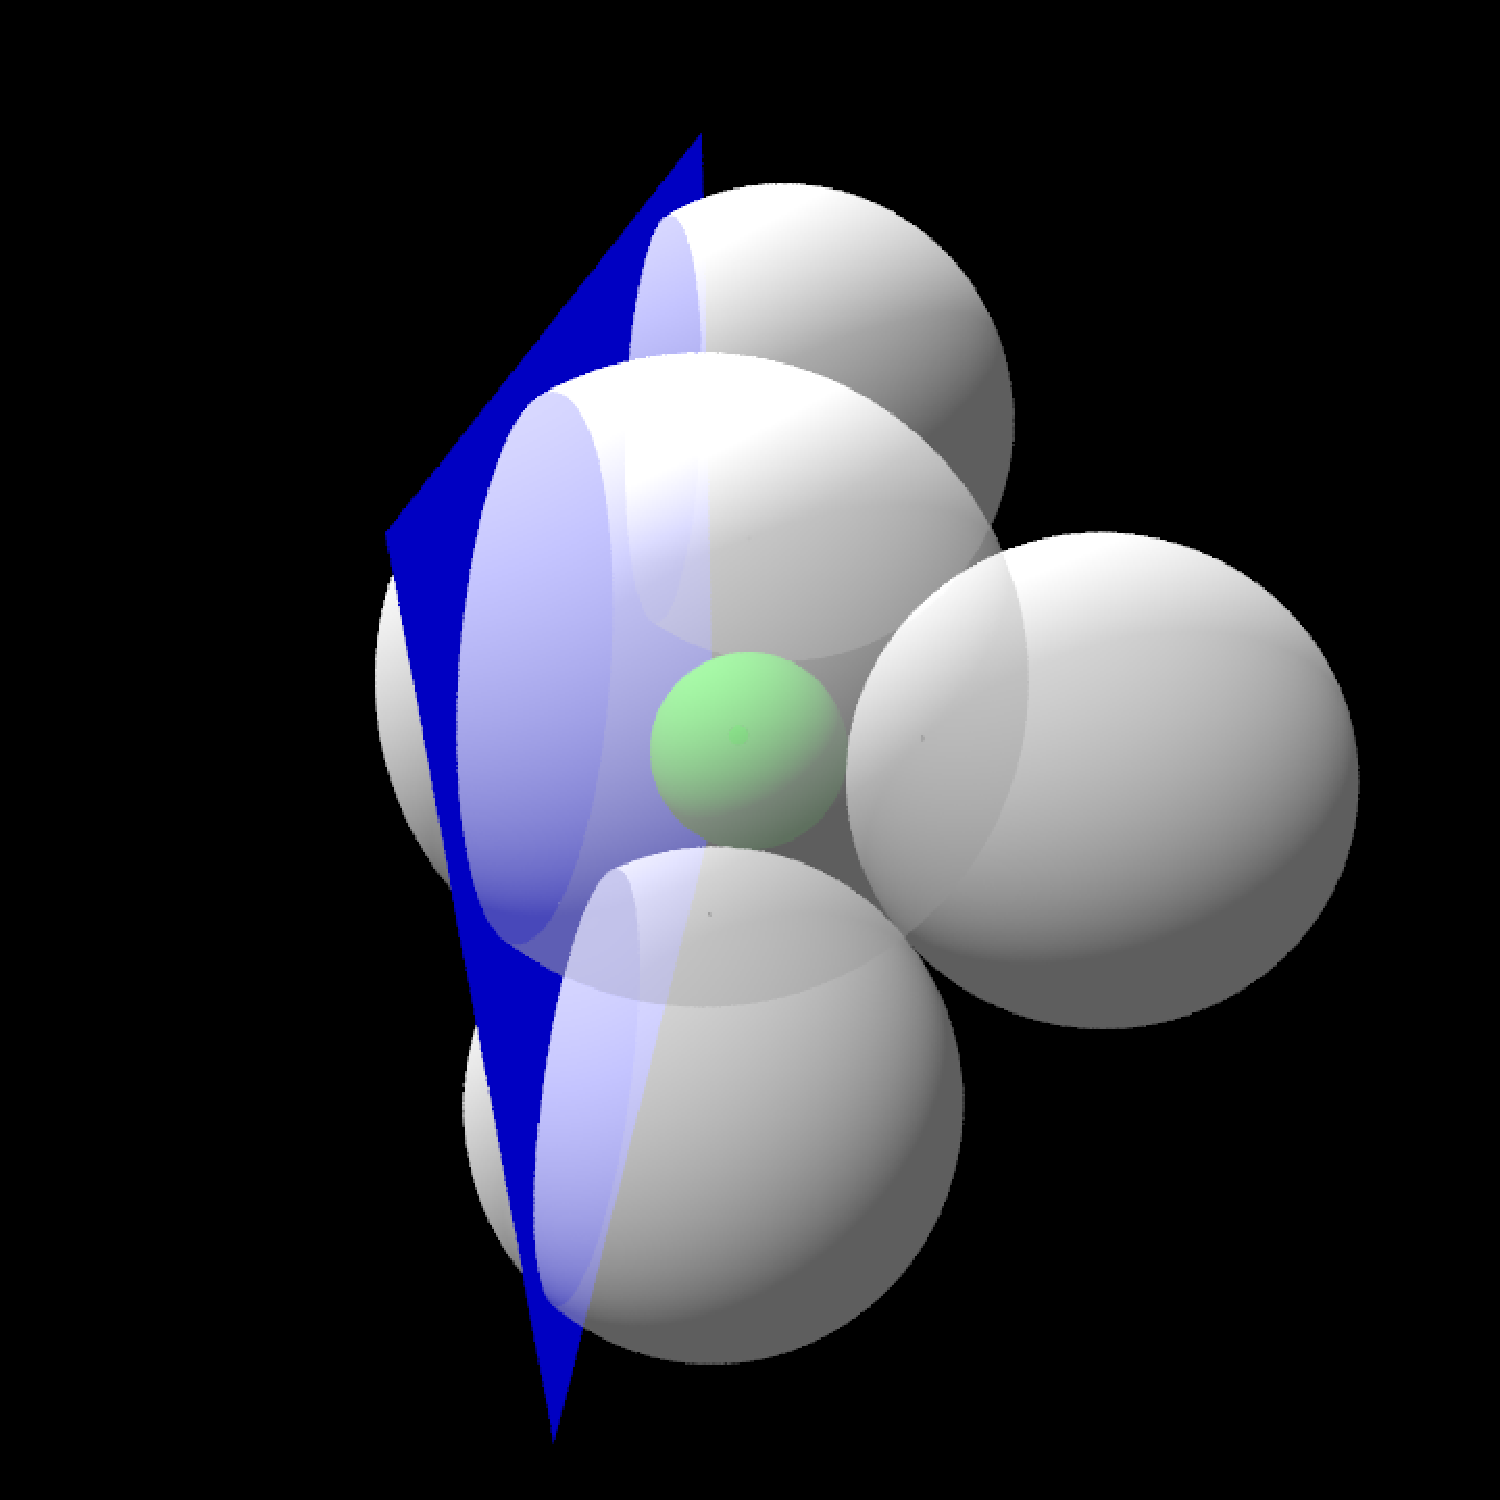
\includegraphics[width=1.4in, height=1.4in, keepaspectratio]{./img/application/3dGen/infSphereGen.pdf}
   \subcaption{\textit{Generator}}
   \label{fig:infSphereGen}
  \end{minipage}
  \hspace*{\fill}
  \begin{minipage}{0.25\hsize}
   \center
   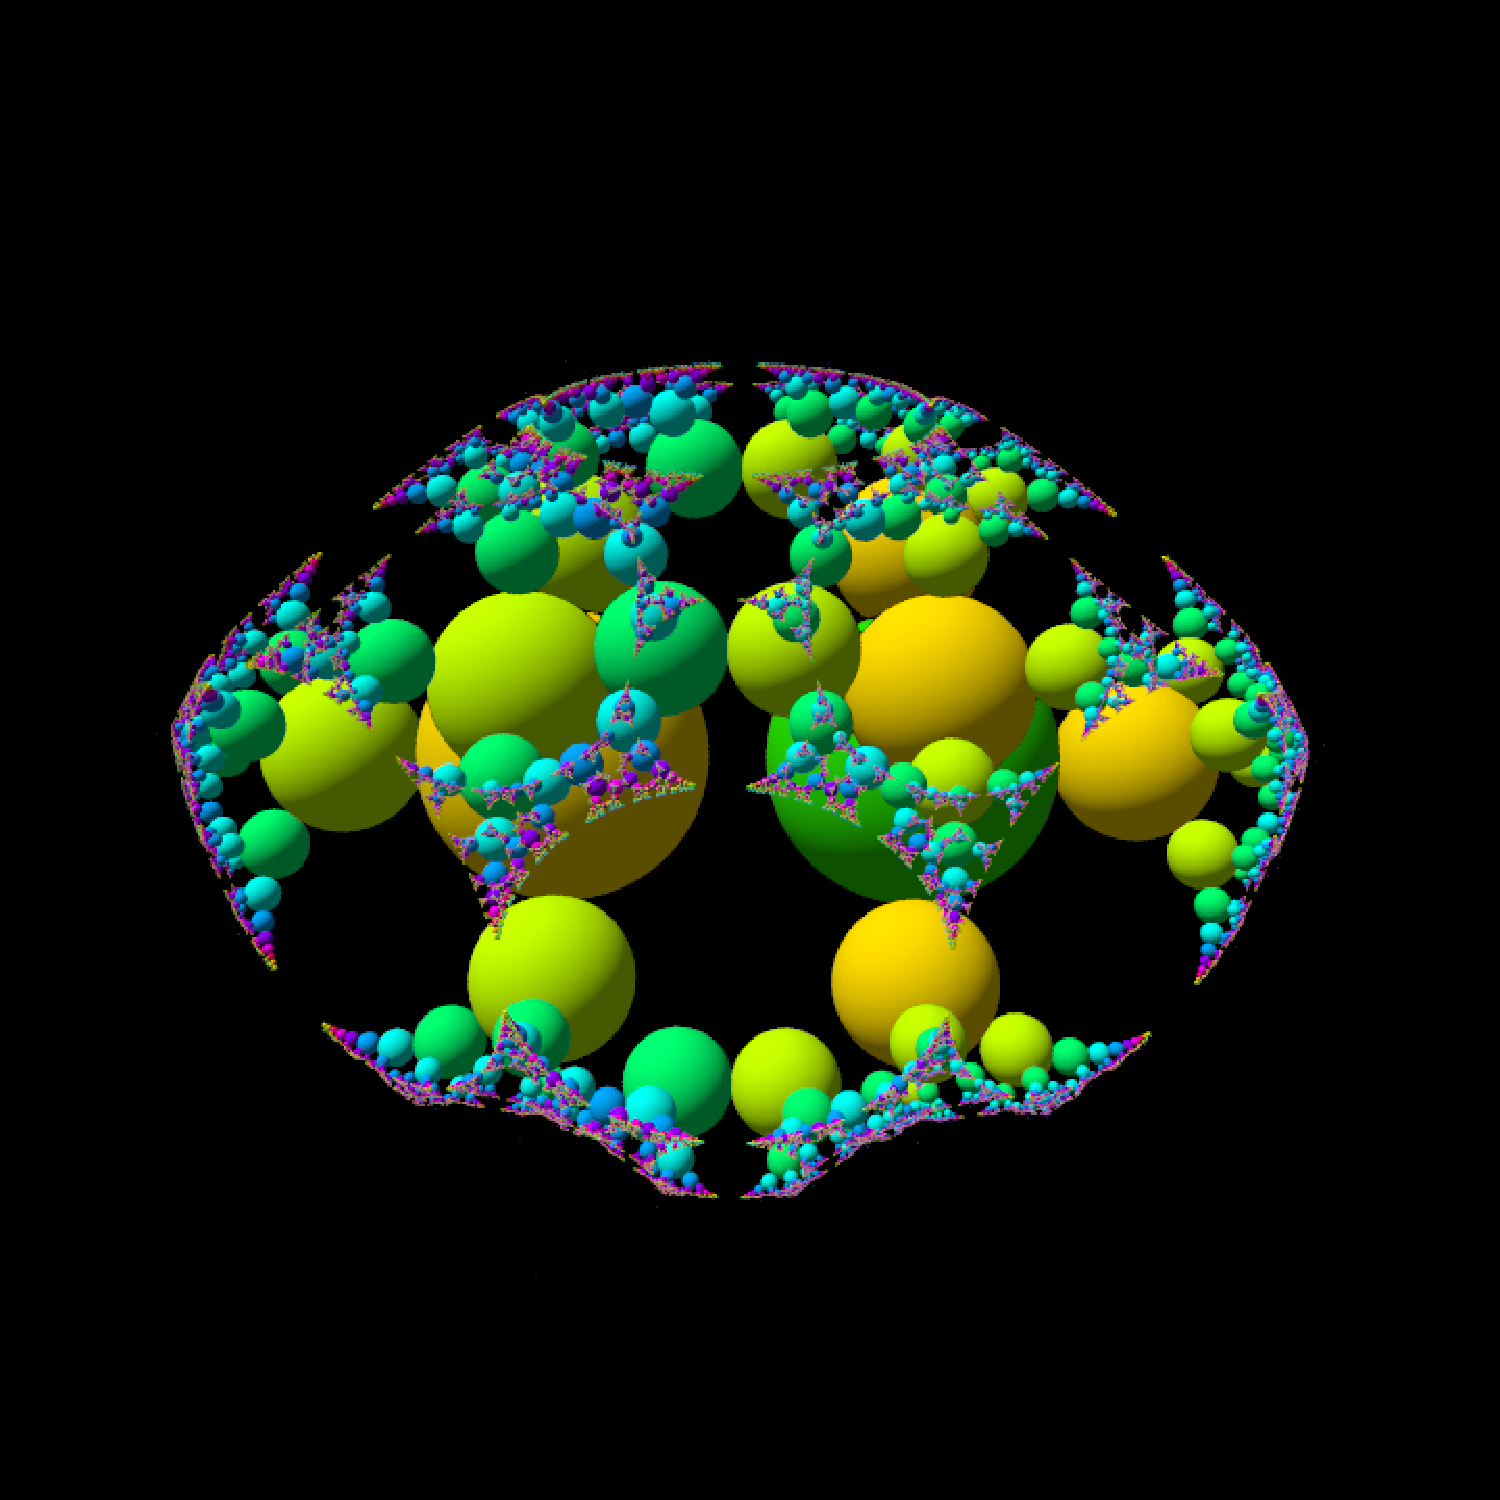
\includegraphics[width=1.4in, height=1.4in, keepaspectratio]{./img/application/3dGen/infSphereOrbit.pdf}
   \subcaption{\textit{Orbit}}
   \label{fig:infSphereOrb}
  \end{minipage}
  \hspace*{\fill}
  \caption{\textit{Inversion in the sphere with infinite radius, four
  Schottky spheres, and a base sphere}}
  \label{fig:infSphere}
 \end{minipage}
 \hspace*{\fill}
 \begin{minipage}[t]{0.5\hsize}
  \begin{minipage}{0.25\hsize}
   \center
   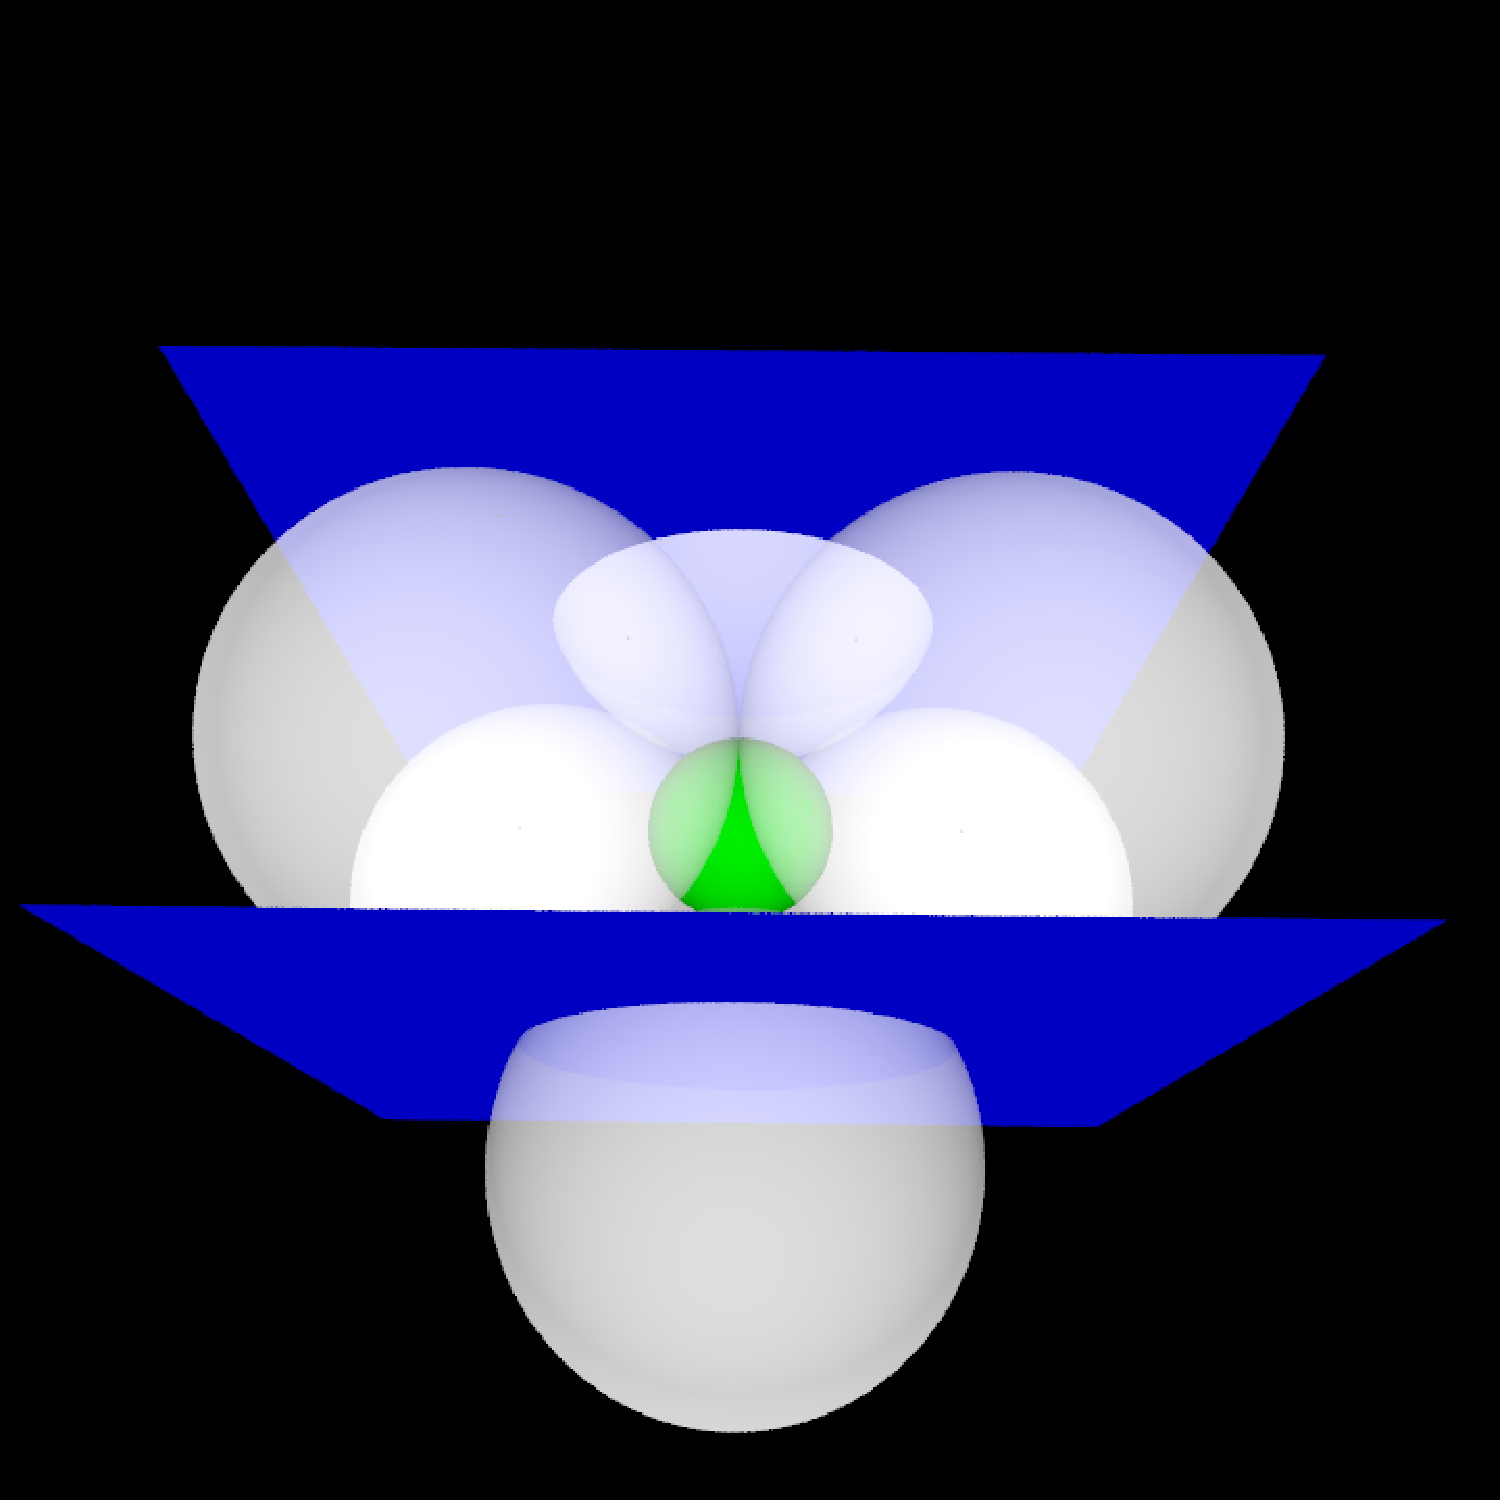
\includegraphics[width=1.4in, height=1.4in, keepaspectratio]{./img/application/3dGen/translationGen.pdf}
   \subcaption{\textit{Generator}}
   \label{fig:translation3dGen}
  \end{minipage}
  \hspace*{\fill}
 \begin{minipage}{0.25\hsize}
  \center
  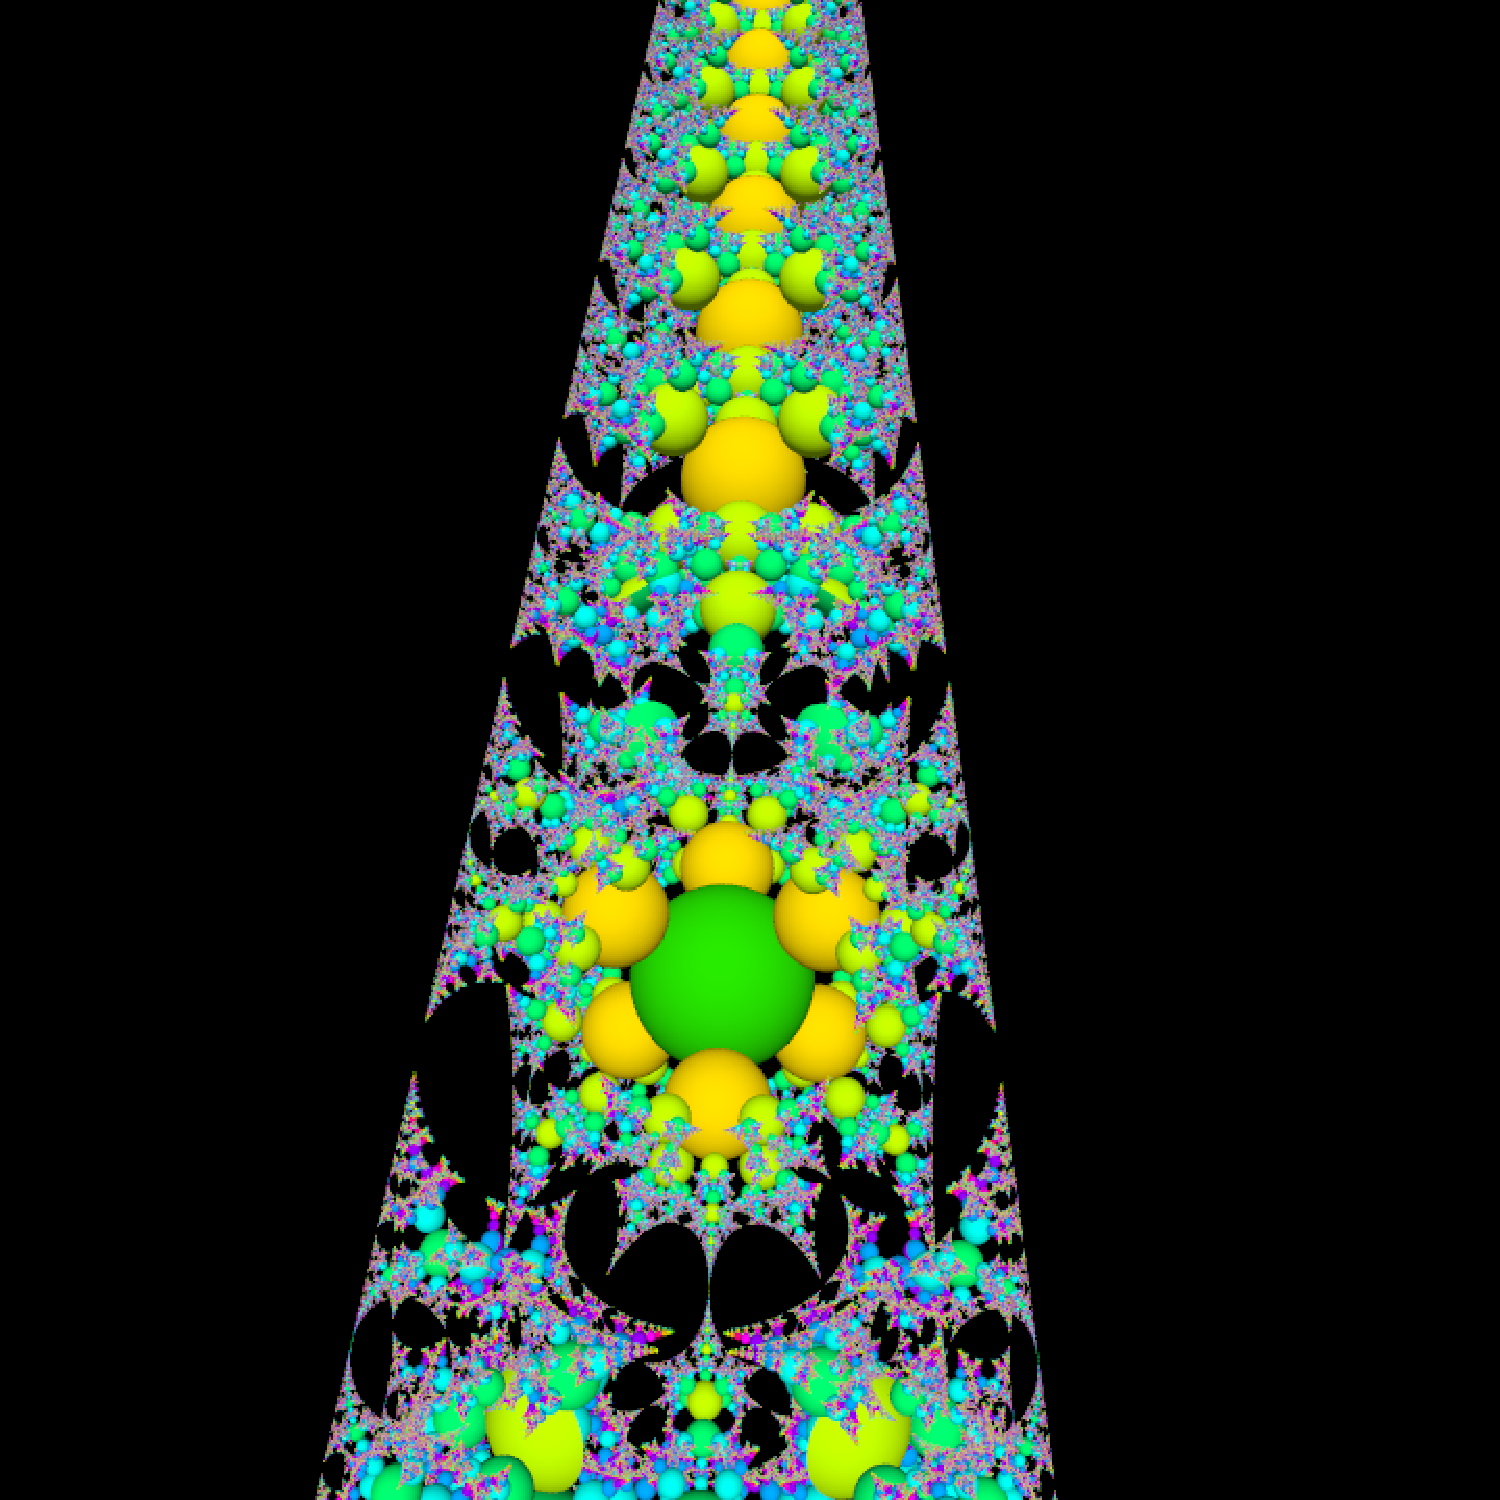
\includegraphics[width=1.4in, height=1.4in, keepaspectratio]{./img/application/3dGen/translationOrbit.pdf}
  \subcaption{\textit{Orbit}}
    \label{fig:translation3dOrb}
 \end{minipage}
  \hspace*{\fill}
  \caption{\textit{Parallel translation generator, six Schottky spheres
  and a base sphere}}
  \label{fig:translation3d}
 \end{minipage}
\end{figure}

\begin{figure}[h!tbp]
 \begin{minipage}[t]{0.5\hsize}
  \begin{minipage}{0.25\hsize}
   \center
    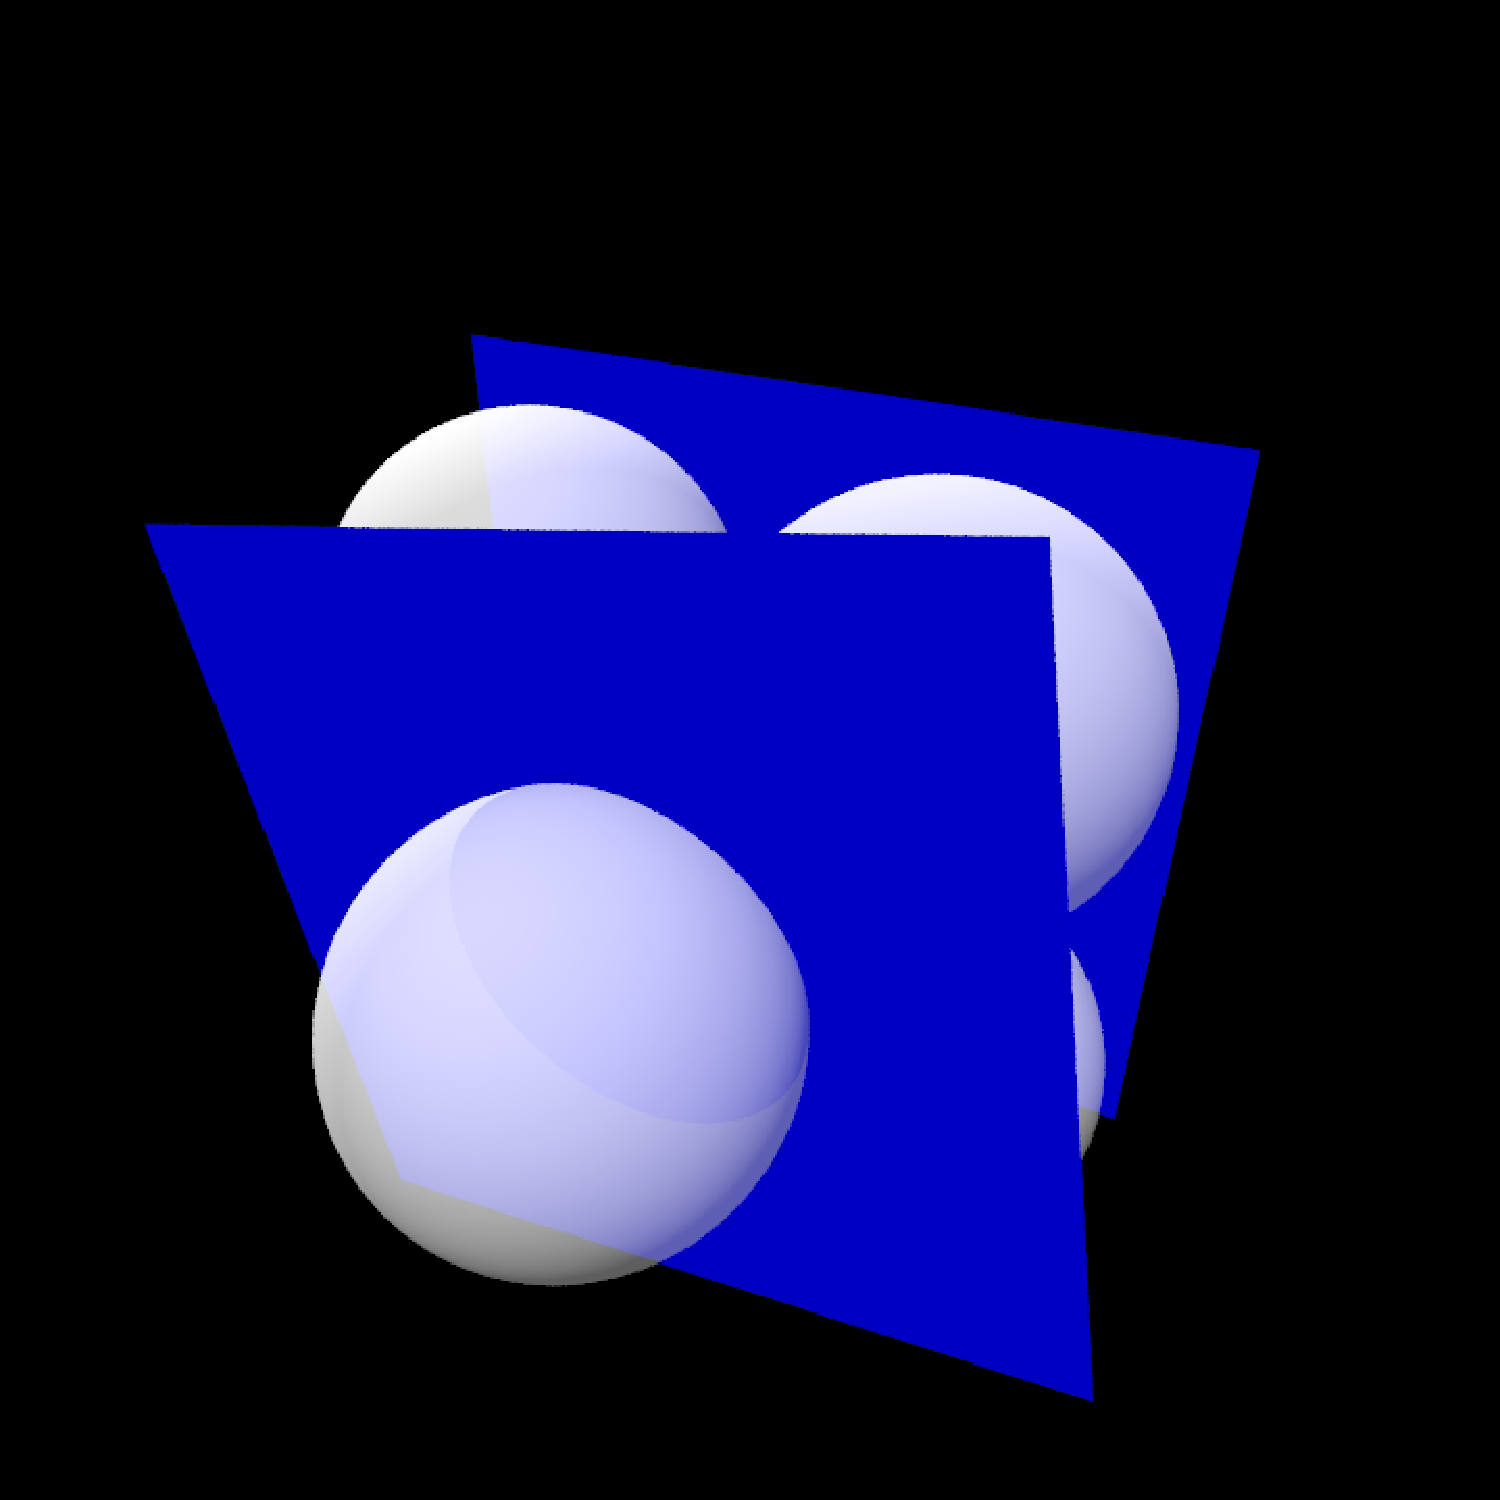
\includegraphics[width=1.4in, height=1.4in, keepaspectratio]{./img/application/3dGen/compParabolicGen.pdf}
    \subcaption{\textit{Generator}}
    \label{fig:compParabolicGen}
  \end{minipage}
  \hspace*{\fill}
  \begin{minipage}{0.25\hsize}
   \center
   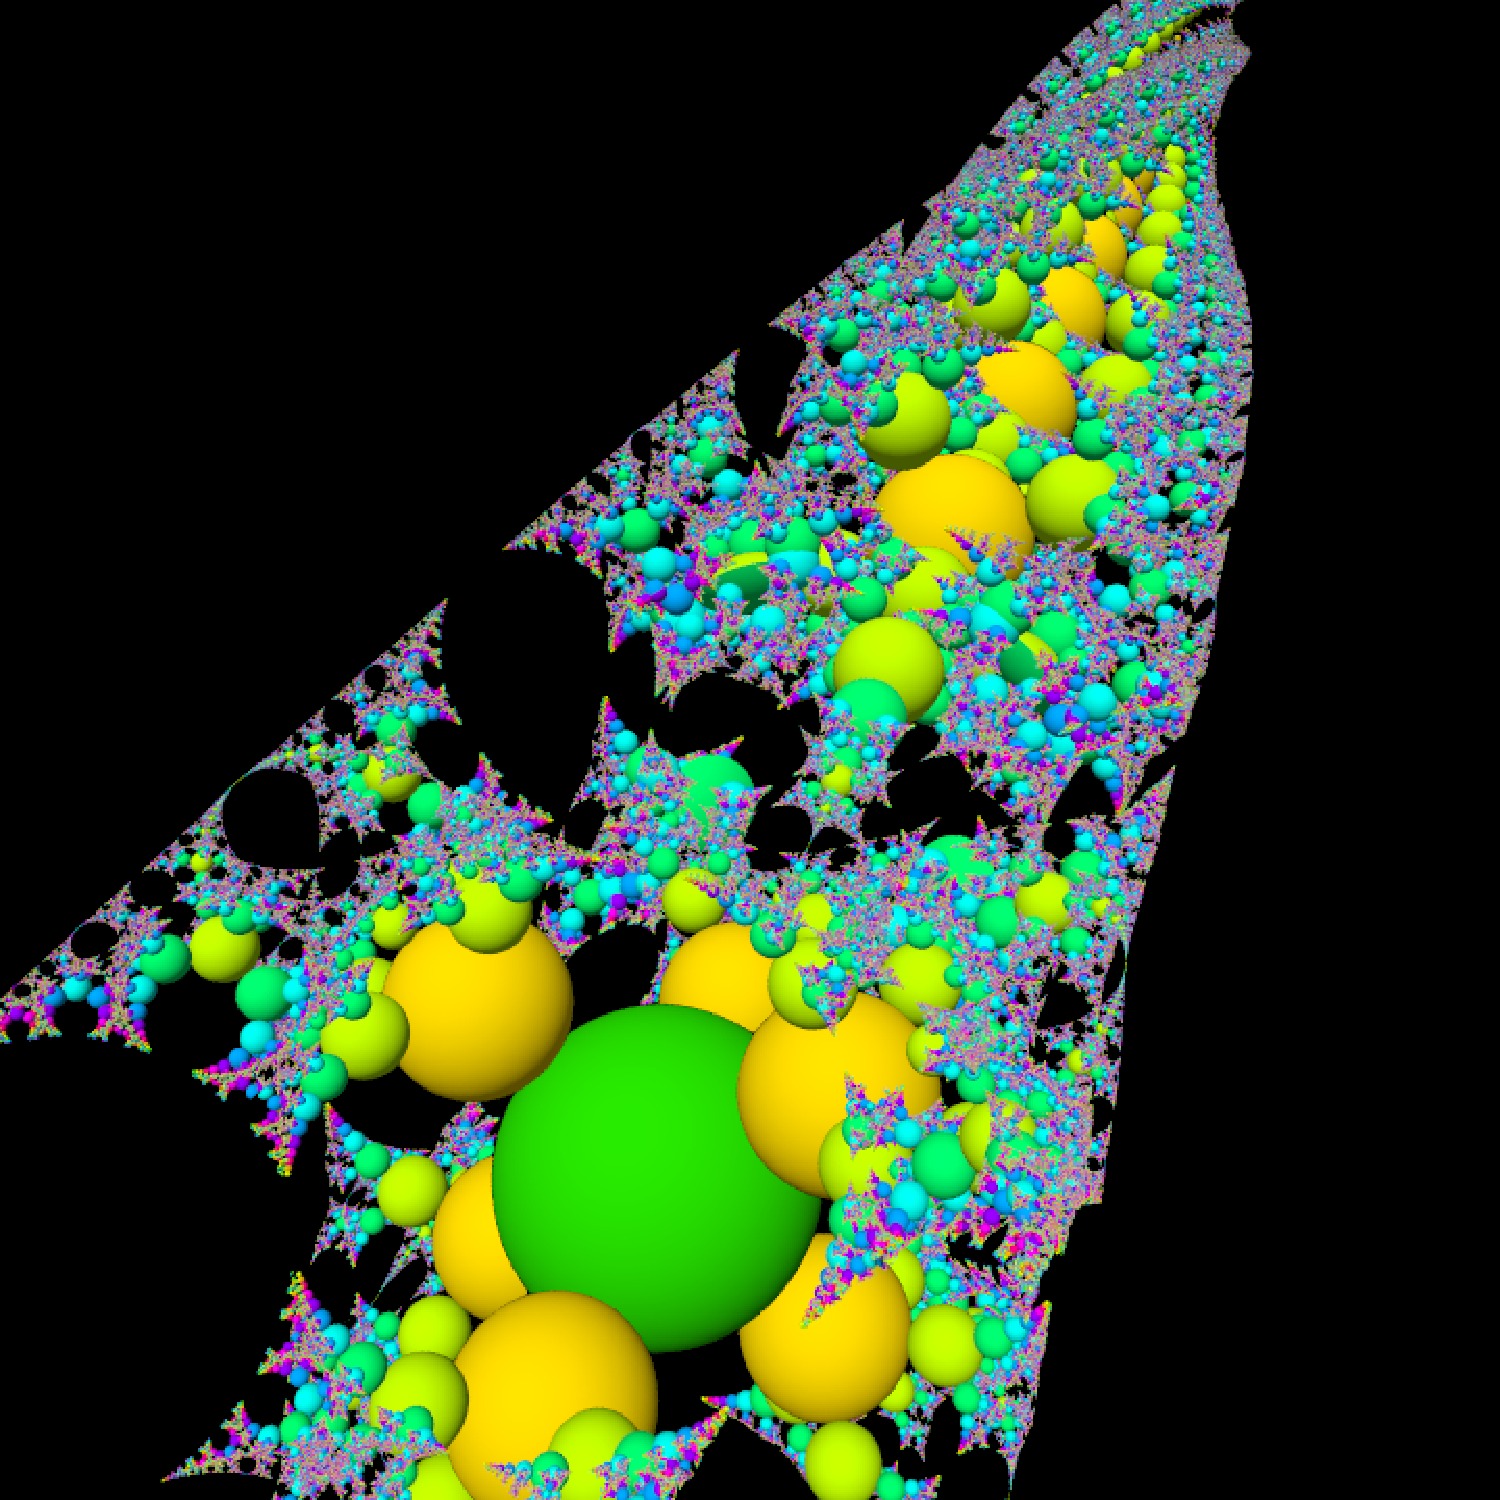
\includegraphics[width=1.4in, height=1.4in, keepaspectratio]{./img/application/3dGen/compParabolicOrb.pdf}
   \subcaption{\textit{Orbit}}
   \label{fig:compParabolicOrb}
  \end{minipage}
  \hspace*{\fill}
  \caption{\textit{Compound parabolic generator, six \\Schottky spheres
  and a base sphere}}
  \label{fig:compParabolic}
 \end{minipage}
 \hspace*{\fill}
 \begin{minipage}[t]{0.5\hsize}
  \begin{minipage}{0.25\hsize}
   \center
   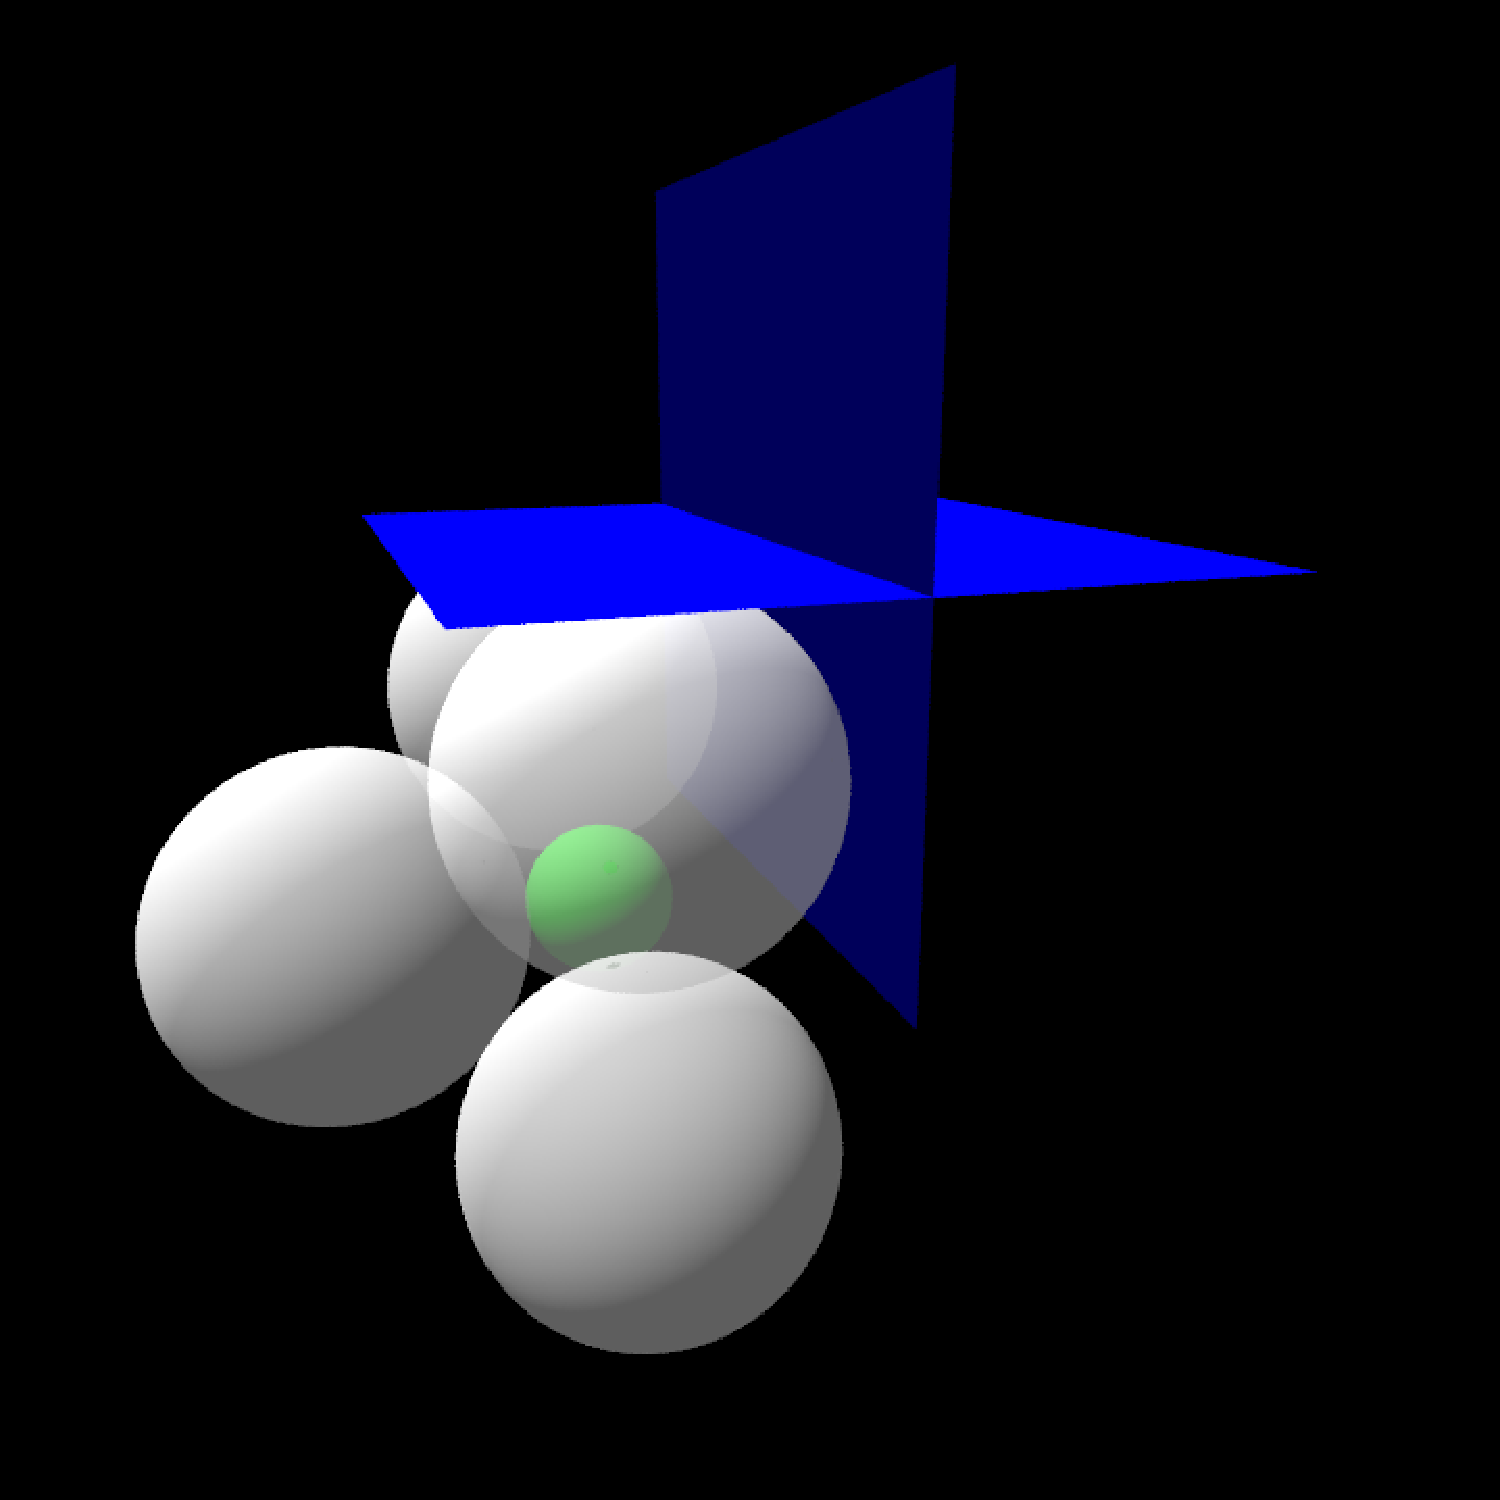
\includegraphics[width=1.4in, height=1.4in, keepaspectratio]{./img/application/3dGen/rotationGen.pdf}
   \subcaption{\textit{Generator}}
   \label{fig:rotationGen}
  \end{minipage}
  \hspace*{\fill}
  \begin{minipage}{0.25\hsize}
   \center
   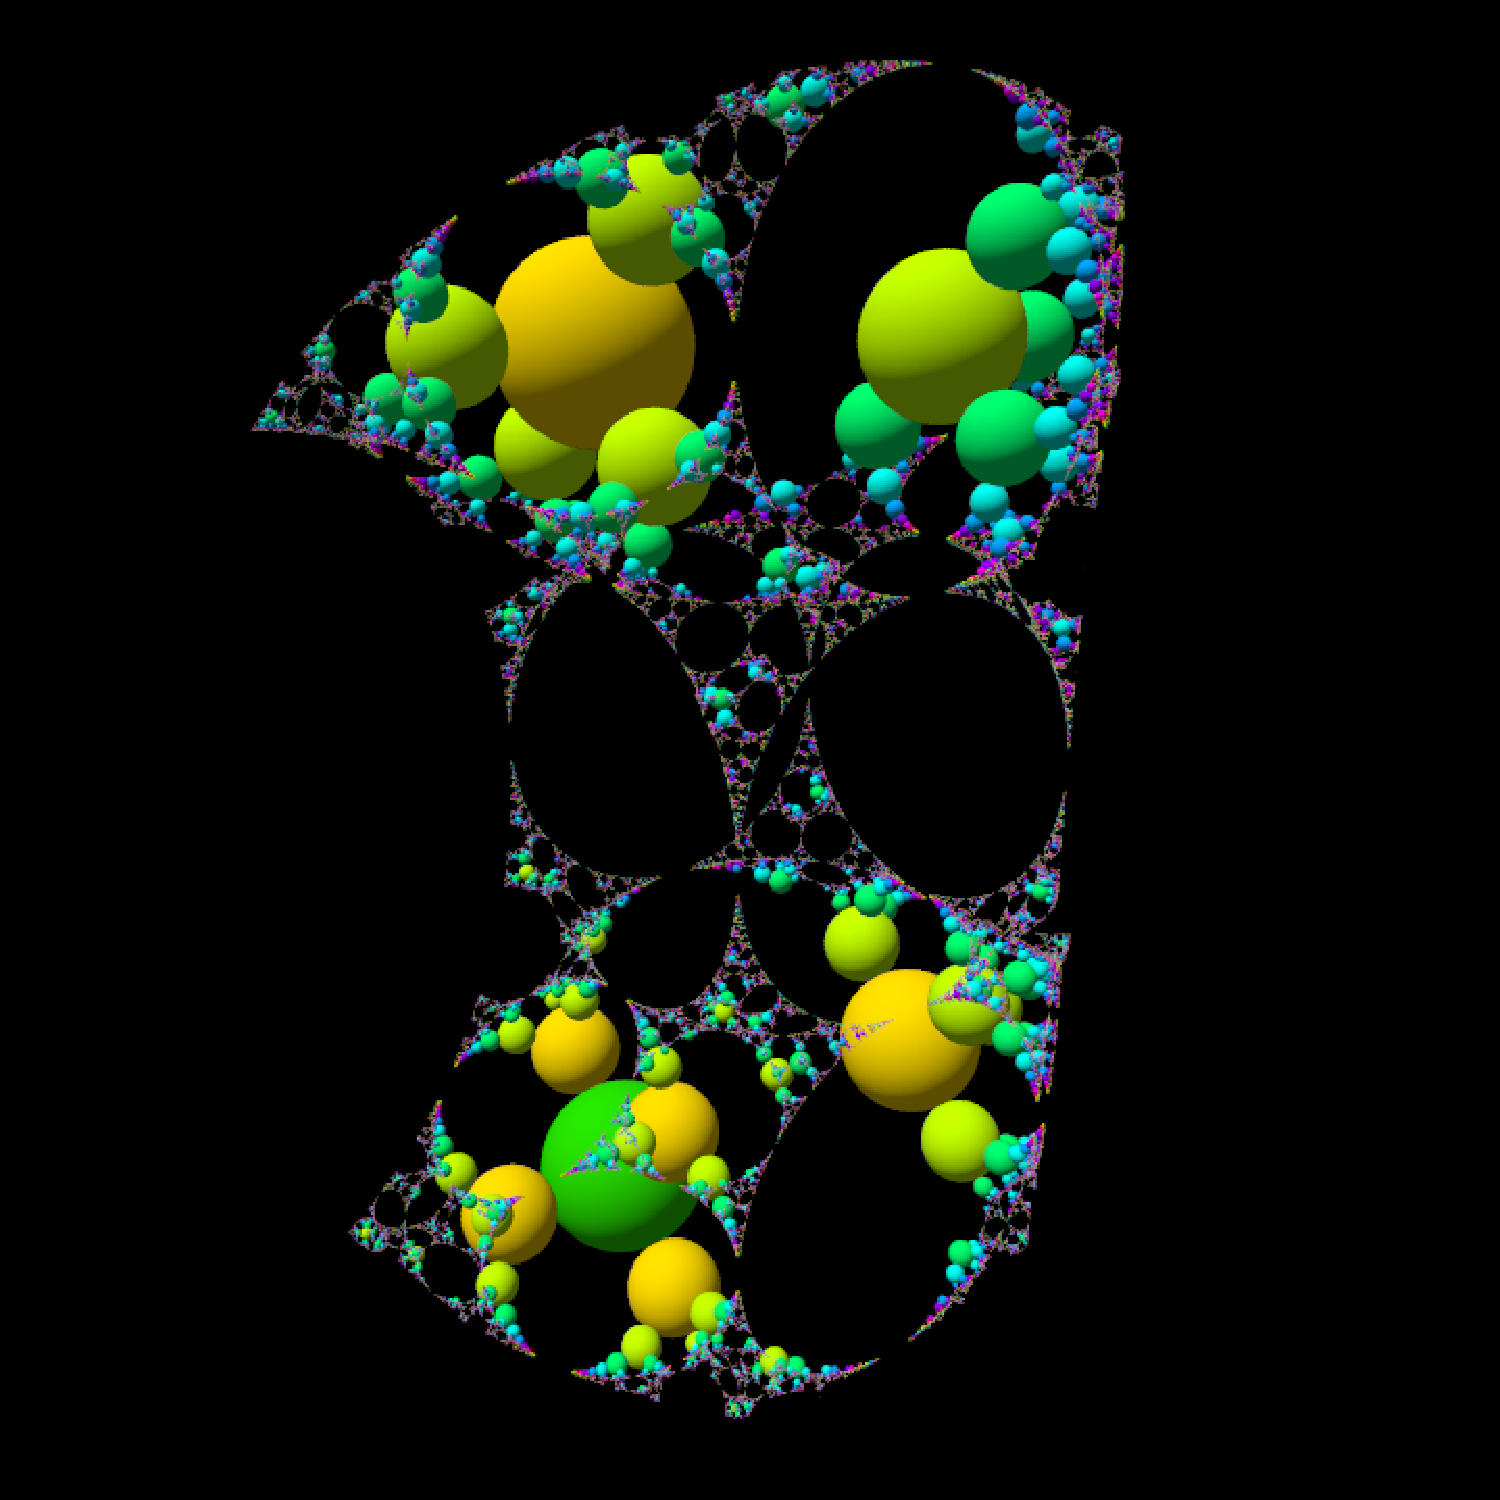
\includegraphics[width=1.4in, height=1.4in, keepaspectratio]{./img/application/3dGen/rotationOrb.pdf}
   \subcaption{\textit{Orbit}}
   \label{fig:rotationOrb}
  \end{minipage}
  \hspace*{\fill}
  \caption{\textit{Rotation generator, four Schottky spheres, and a base
  sphere}}
  \label{fig:rotation3d}
 \end{minipage}
\end{figure}

\begin{figure}[h!tbp]
 \begin{minipage}{0.5\hsize}
  \begin{minipage}{0.25\hsize}
   \center
   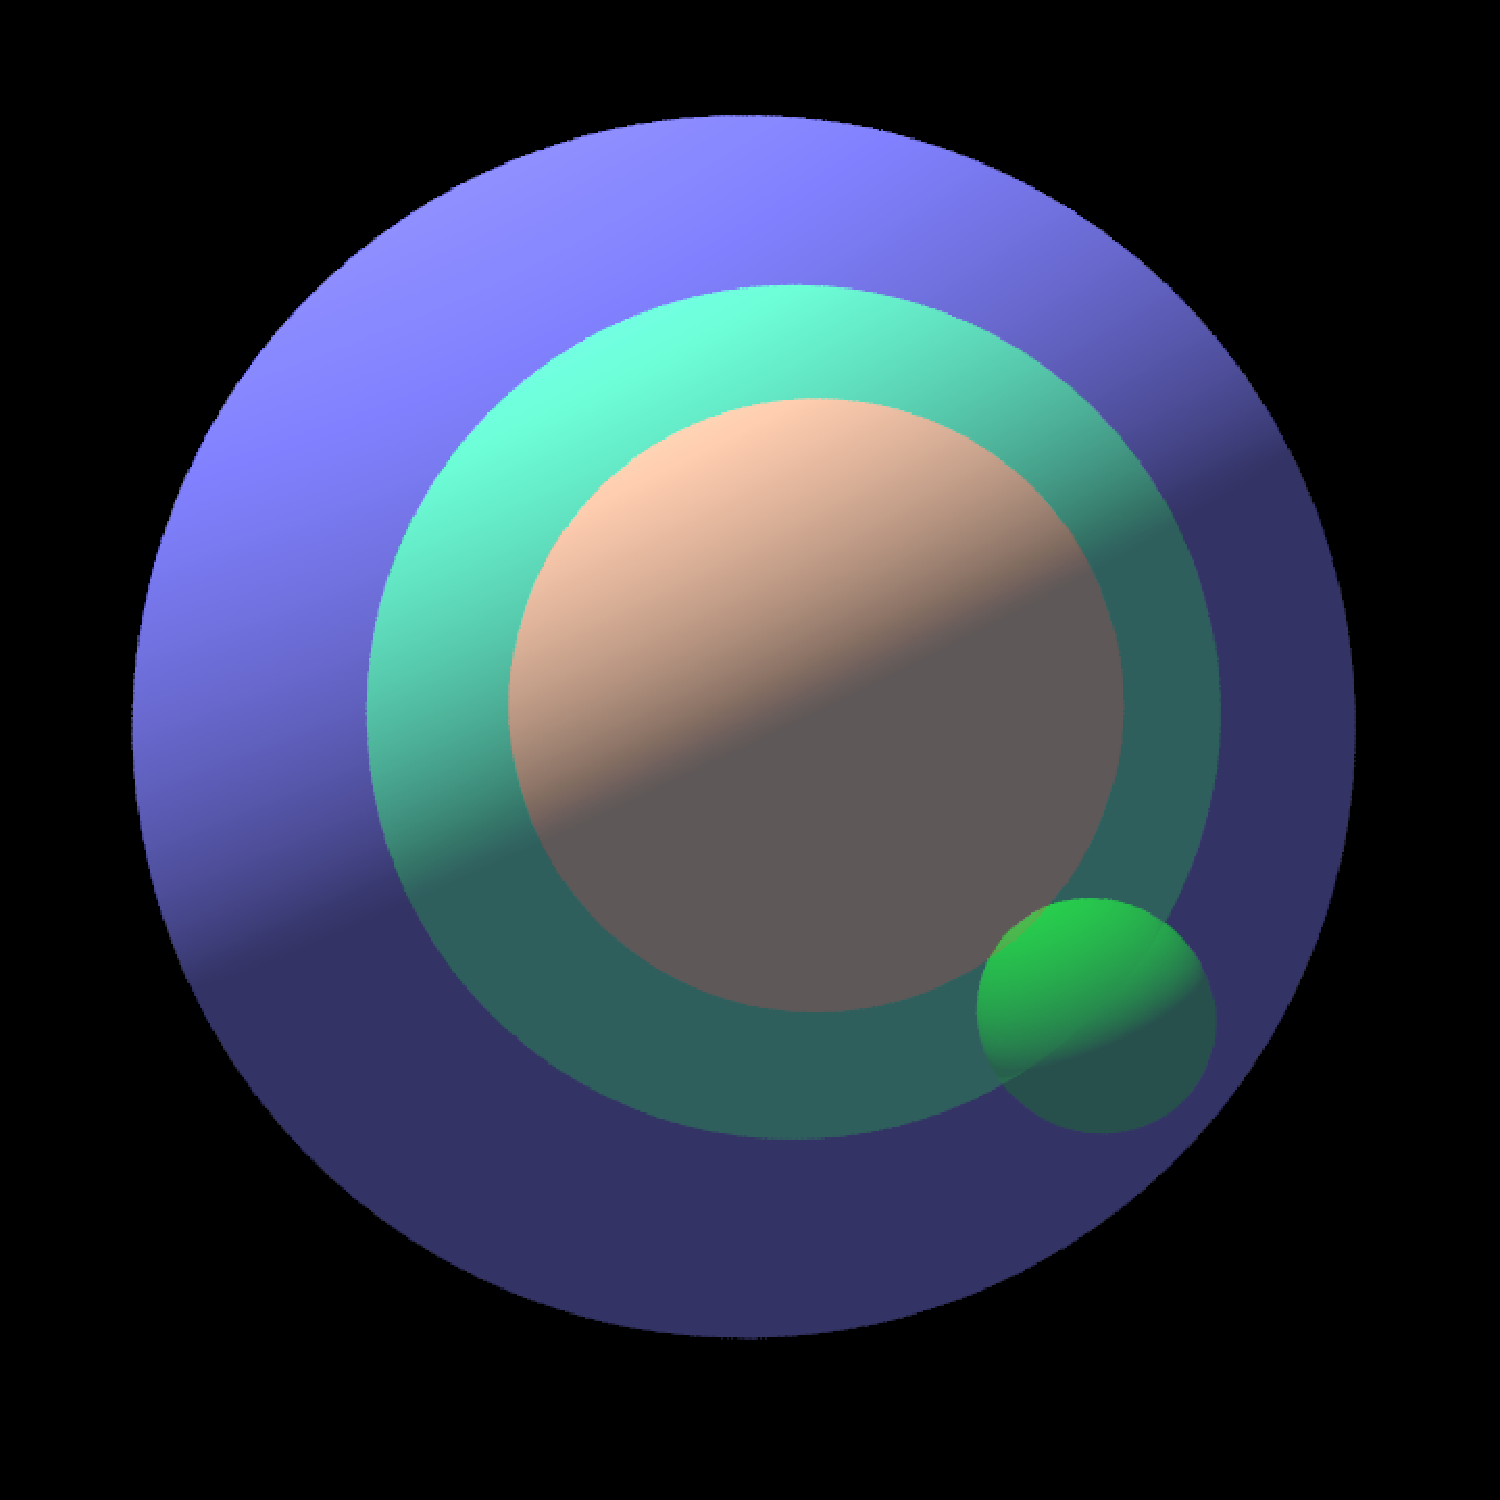
\includegraphics[width=1.4in, height=1.4in, keepaspectratio]{./img/application/3dGen/loxoGenSimple.pdf}
   \subcaption{\textit{Generator}}
   \label{fig:loxoGen3d}
  \end{minipage}
  \hspace*{\fill}
  \begin{minipage}{0.25\hsize}
   \center
   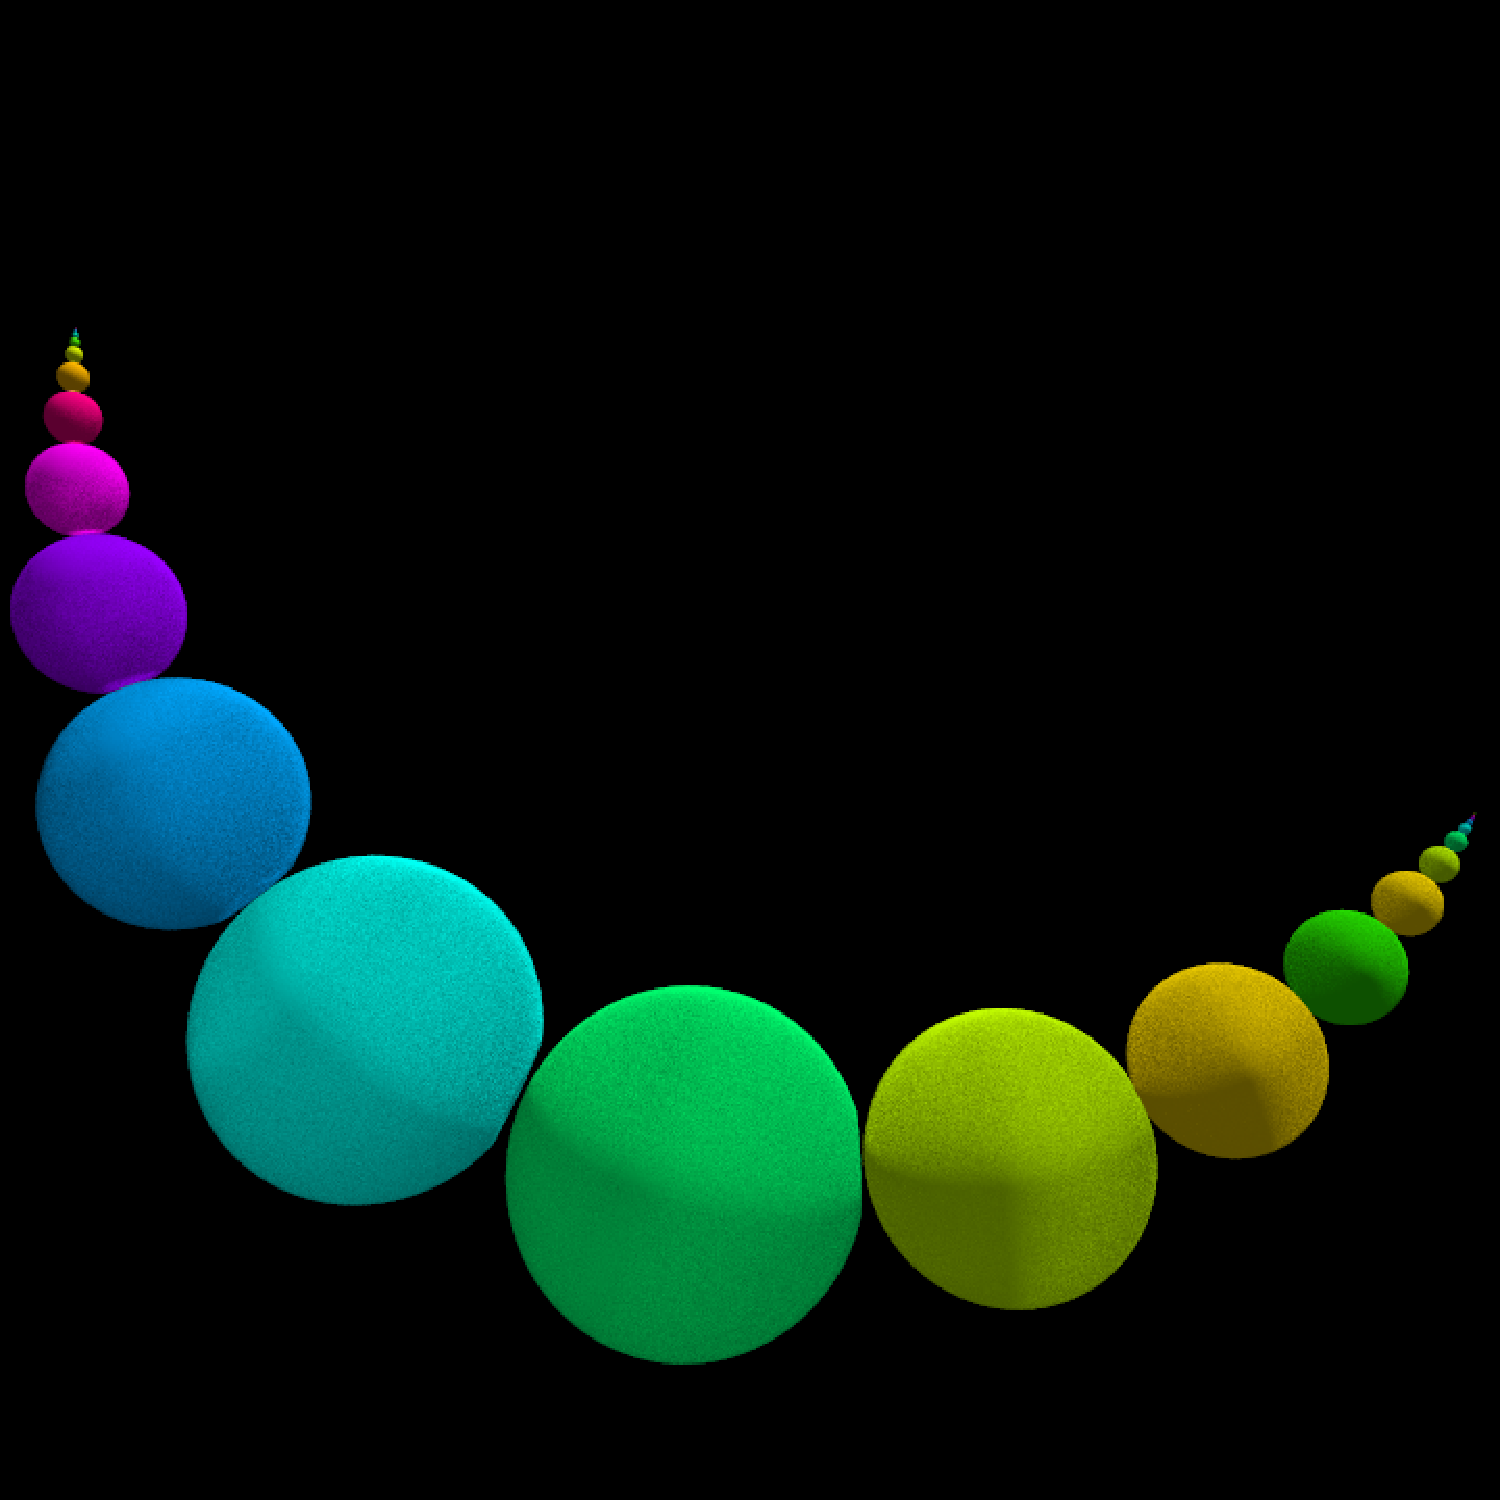
\includegraphics[width=1.4in, height=1.4in, keepaspectratio]{./img/application/3dGen/loxoOrbSimple.pdf}
   \subcaption{\textit{Orbit}}
   \label{fig:loxoOrb3d}
  \end{minipage}
  \hspace*{\fill}
 \caption{\textit{Hyperbolic generator and a base sphere}}
  \label{fig:loxo3d}
 \end{minipage}
 \hspace*{\fill}
 \begin{minipage}{0.5\hsize}
  \begin{minipage}{0.25\hsize}
   \center
   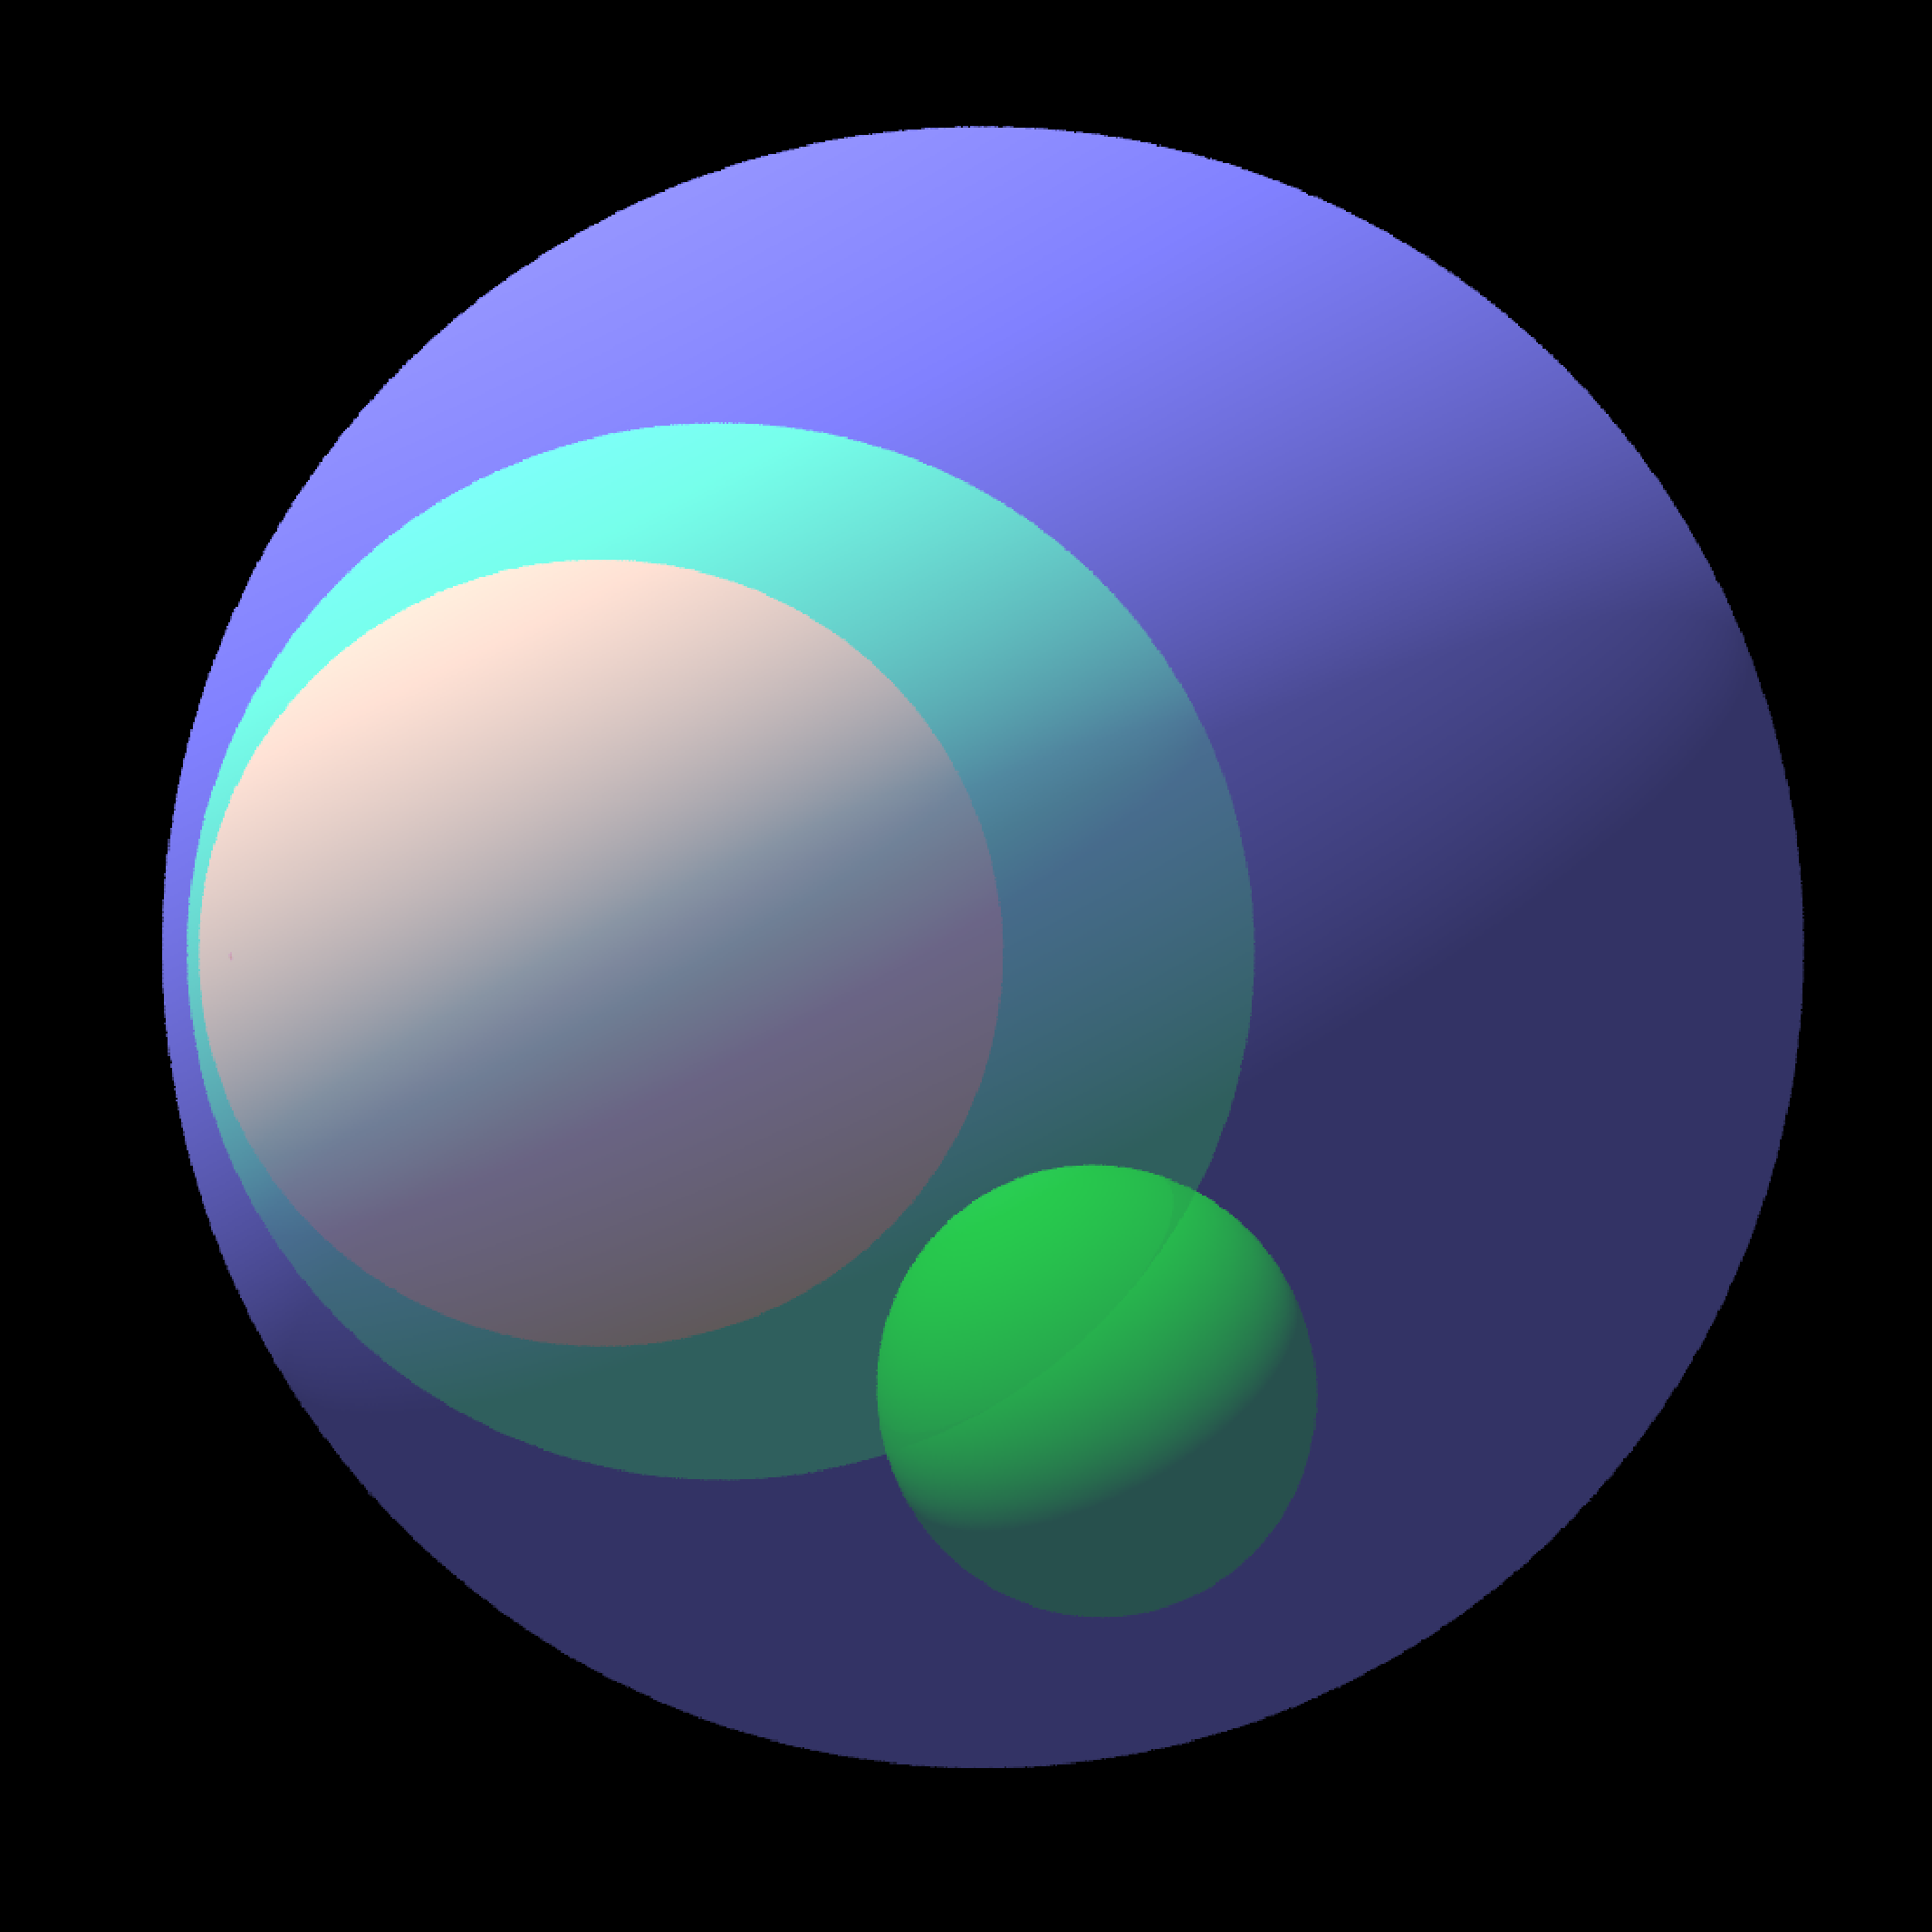
\includegraphics[width=1.4in, height=1.4in, keepaspectratio]{./img/application/3dGen/parabolicOneGen.pdf}
   \subcaption{\textit{Generator}}
   \label{fig:parabolic3dGen}
  \end{minipage}
  \hspace*{\fill}
  \begin{minipage}{0.25\hsize}
   \center
   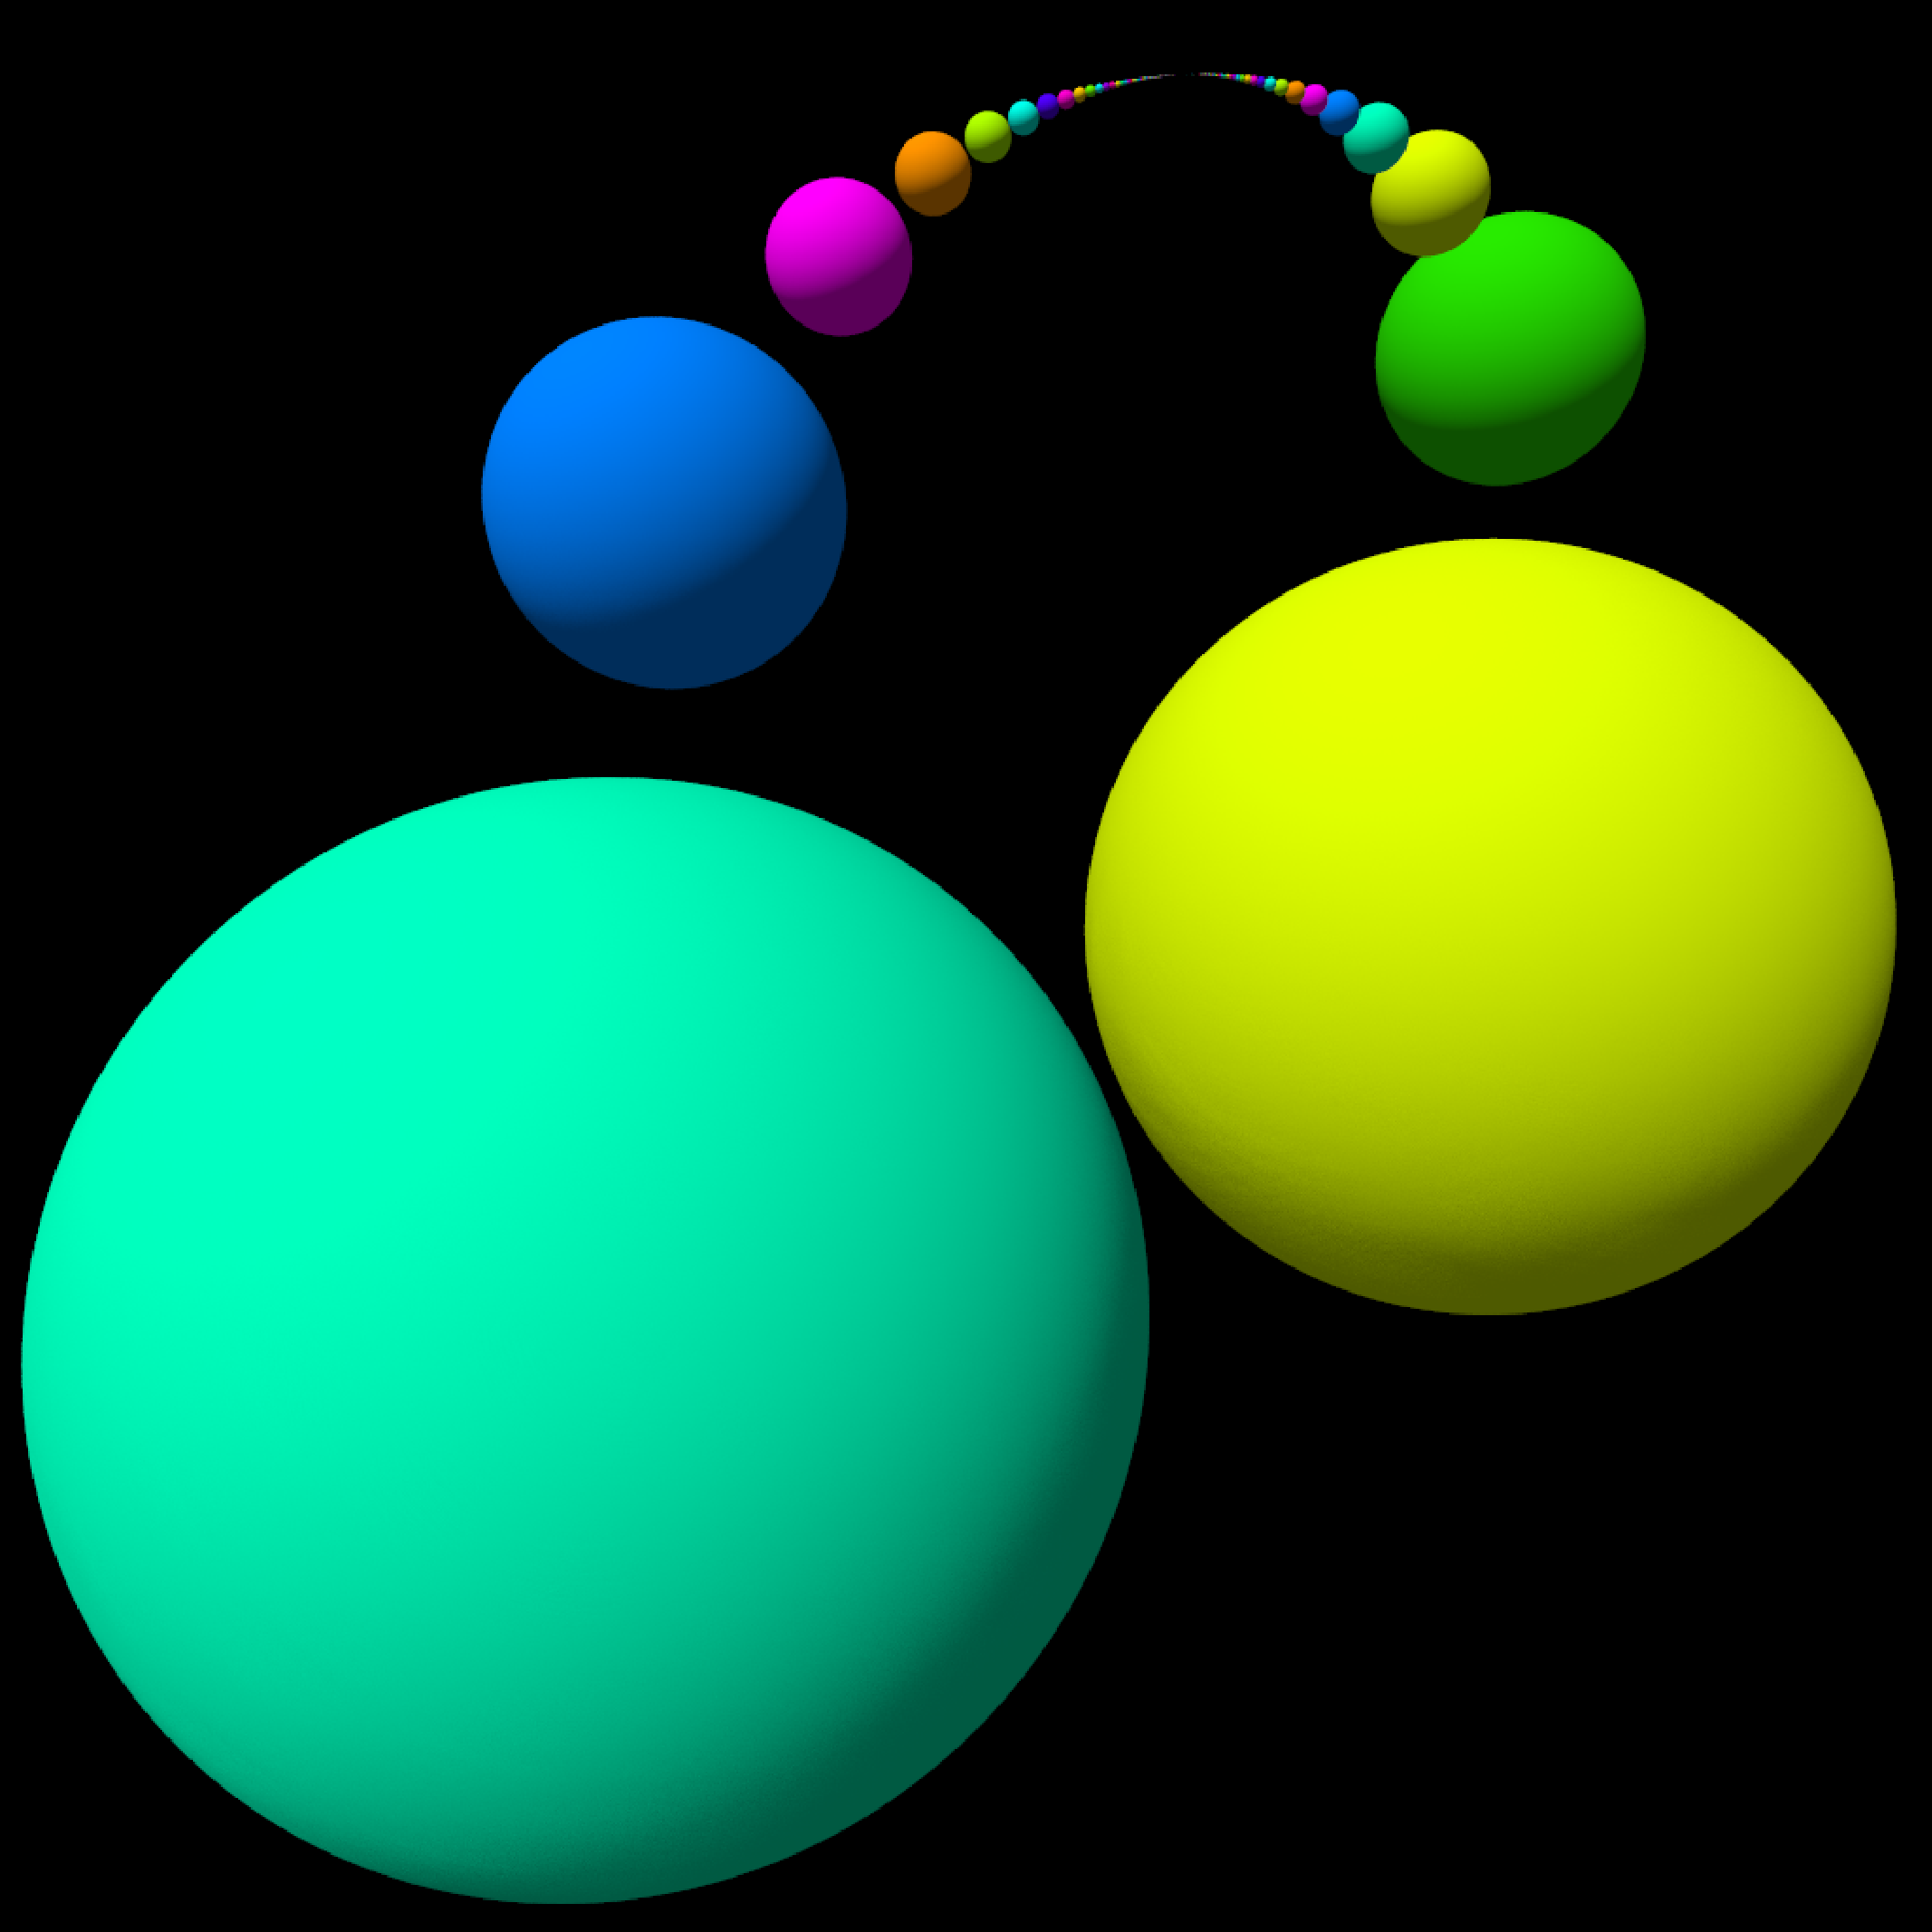
\includegraphics[width=1.4in, height=1.4in, keepaspectratio]{./img/application/3dGen/parabolicOneOrb.pdf}
  \subcaption{\textit{Orbit}}
   \label{fig:parabolic3dOrb}
  \end{minipage}
  \hspace*{\fill}
  \caption{\textit{Parabolic generator and a base sphere}}
  \label{fig:parabolic3d}
 \end{minipage}
\end{figure}

\begin{figure}[h!tbp]
 \begin{minipage}[t]{0.5\hsize}
  \begin{minipage}[t]{0.25\hsize}
   \center
   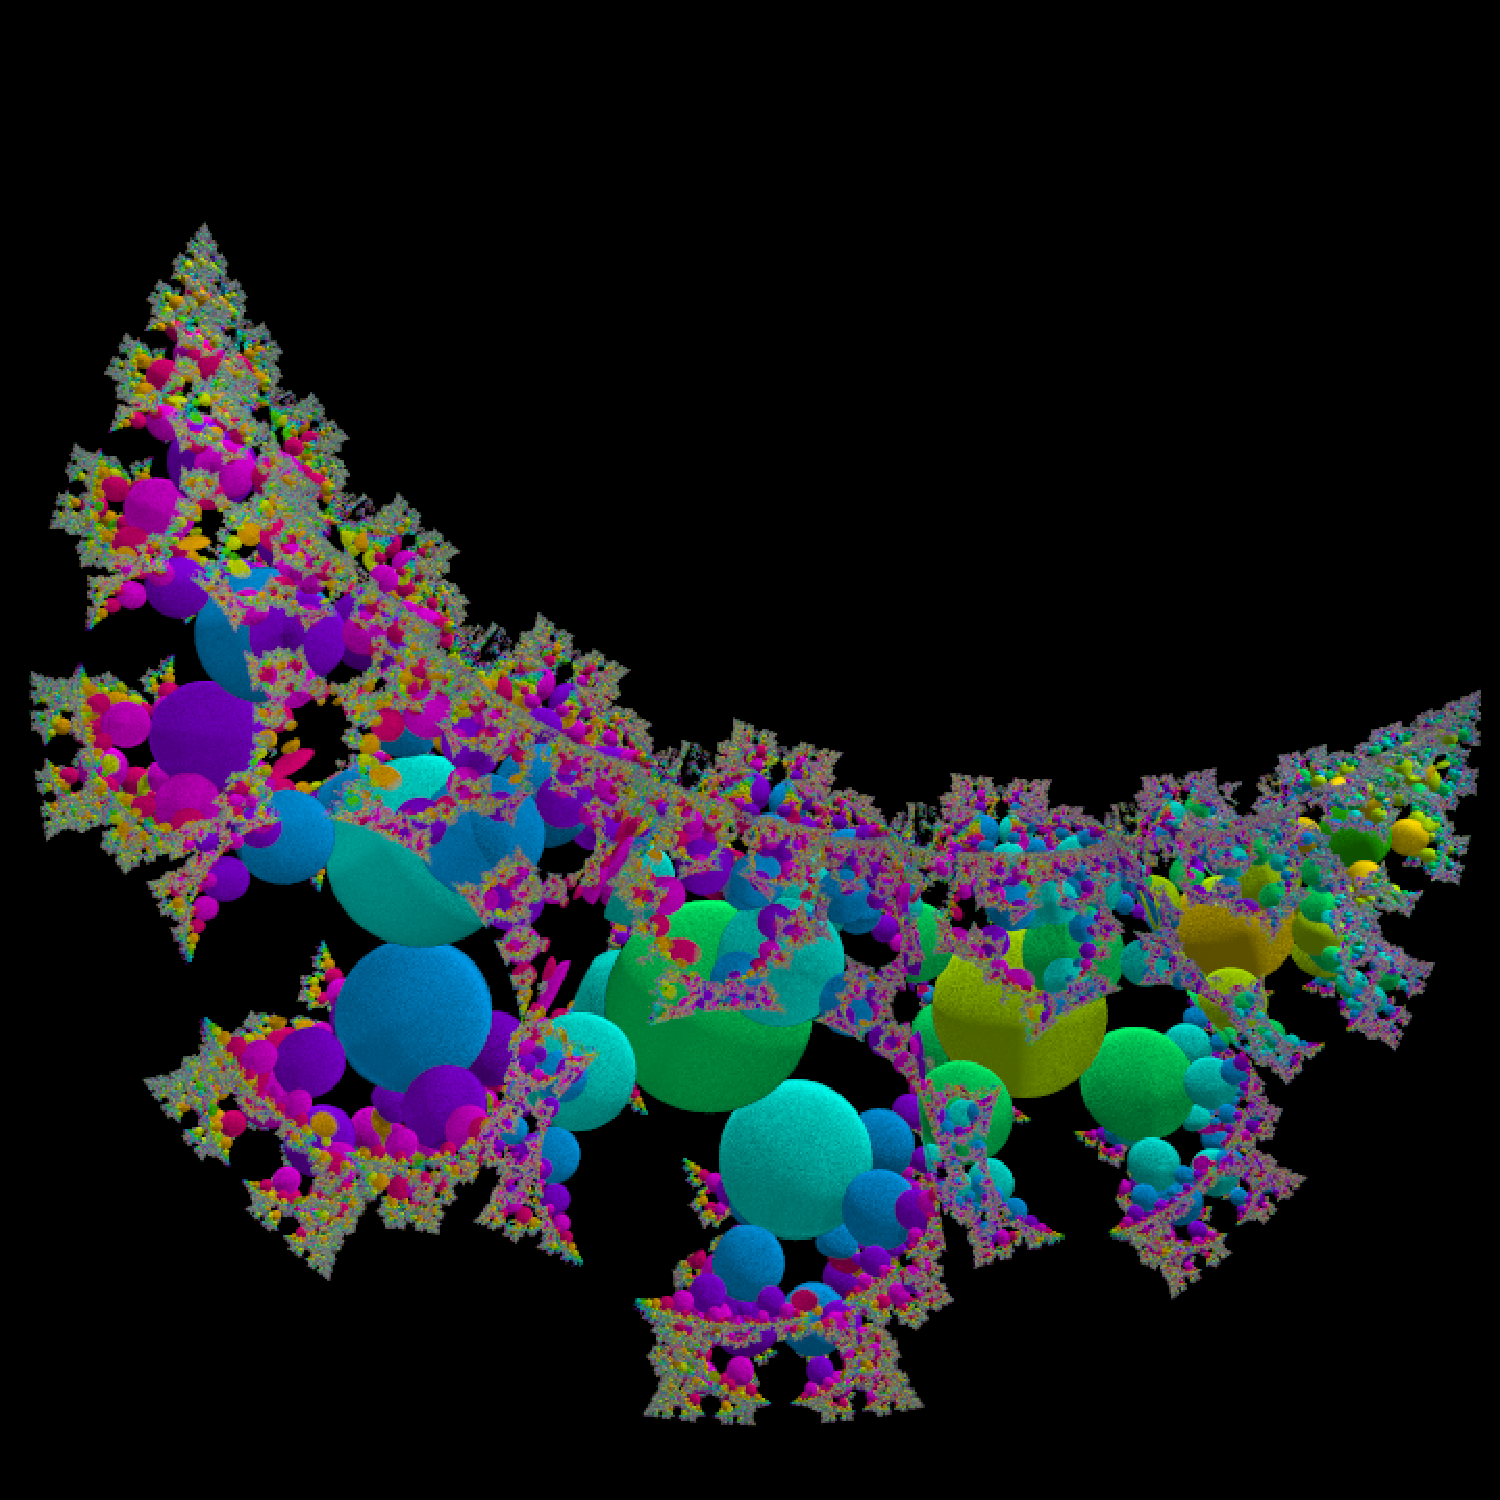
\includegraphics[width=1.4in, height=1.4in, keepaspectratio]{./img/application/3dGen/loxoOrbSch.pdf}
   \subcaption{\textit{Hyperbolic}}
  \end{minipage}
  \hspace*{\fill}
  \begin{minipage}[t]{0.25\hsize}
   \center
   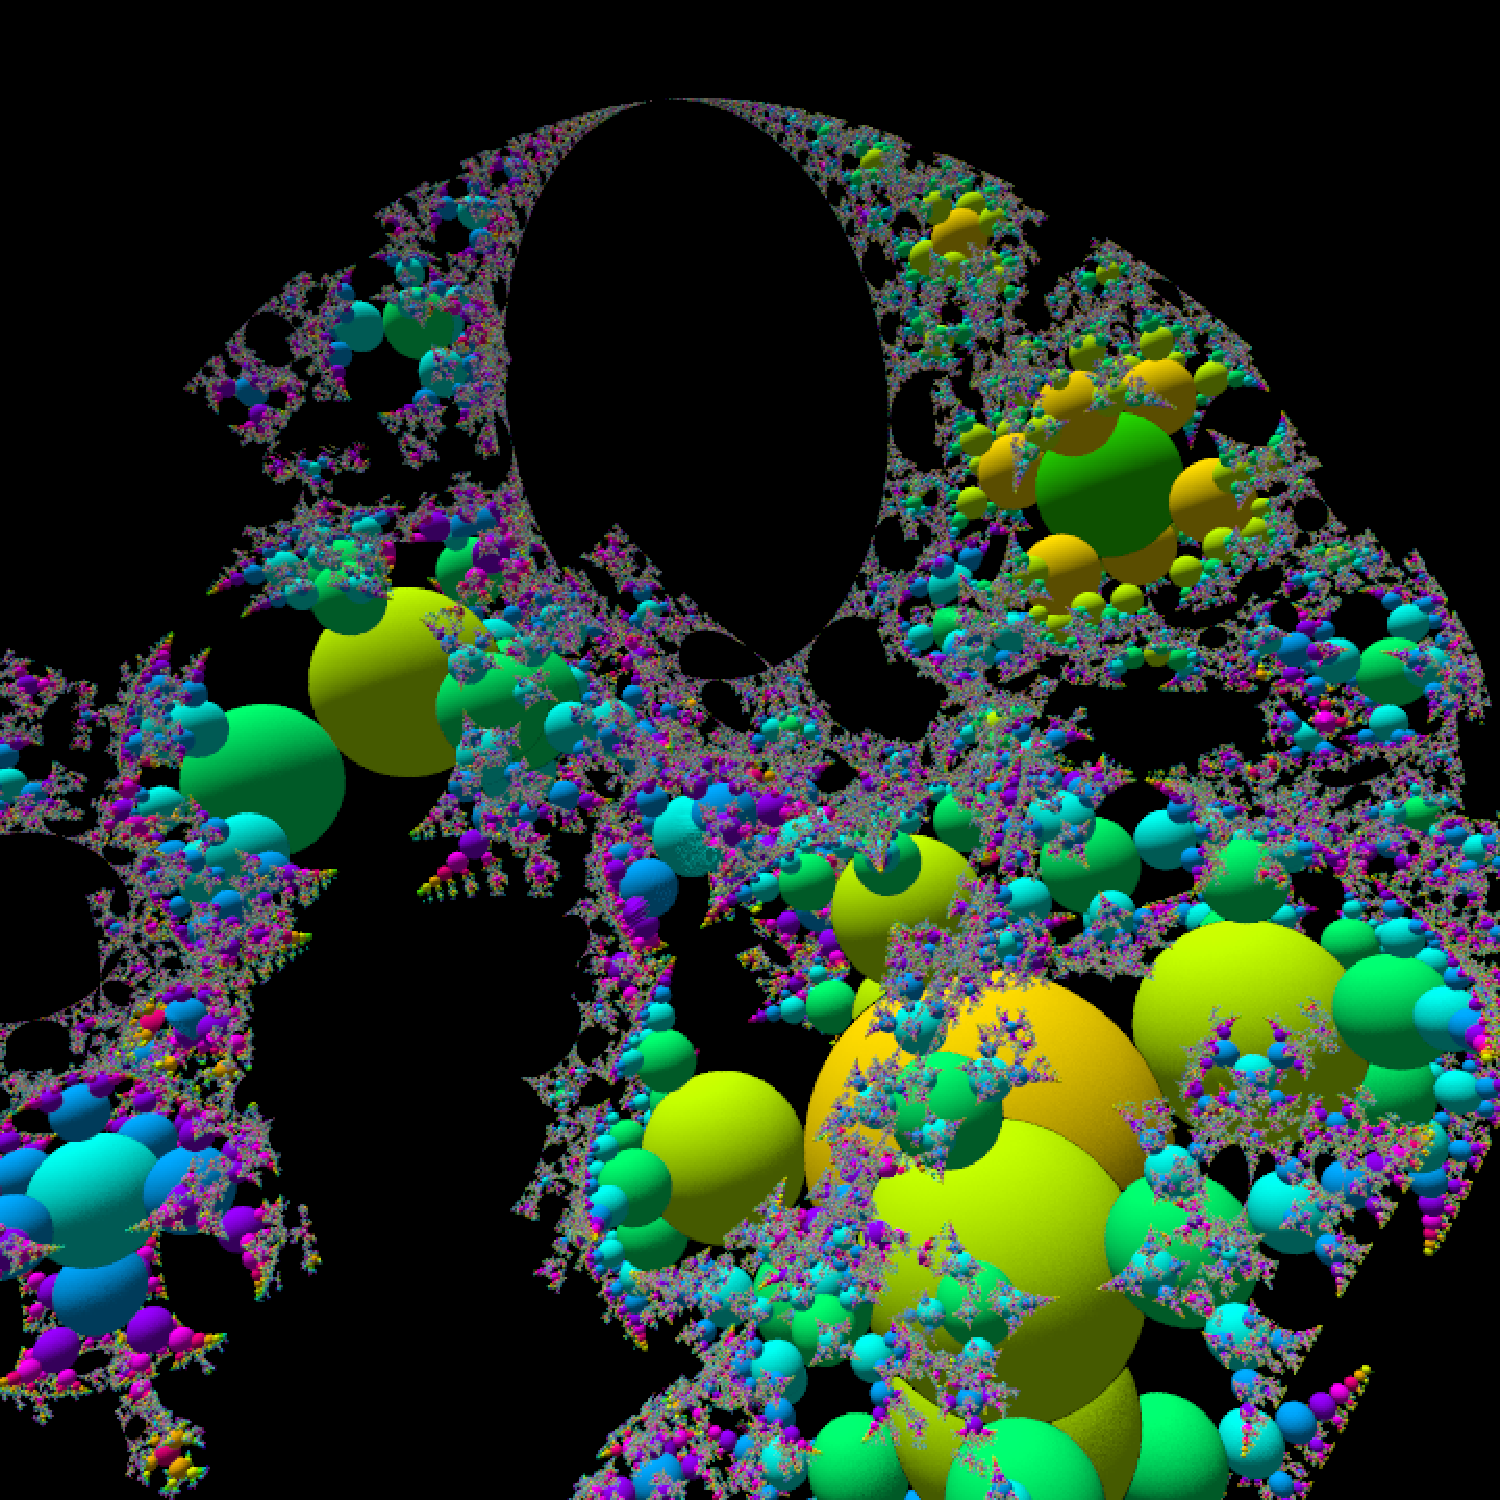
\includegraphics[width=1.4in, height=1.4in, keepaspectratio]{./img/application/3dGen/parabolicOrb.pdf}
   \subcaption{\textit{Parabolic}}
  \end{minipage}
  \hspace*{\fill}
  \caption{\textit{The orbit generated by a composition \\of two spheres and six Schottky
  spheres}}
  \label{fig:complicated3d}
 \end{minipage}
 \hspace*{\fill}
 \begin{minipage}[t]{0.5\hsize}
  \begin{minipage}[t]{0.25\hsize}
   \center
   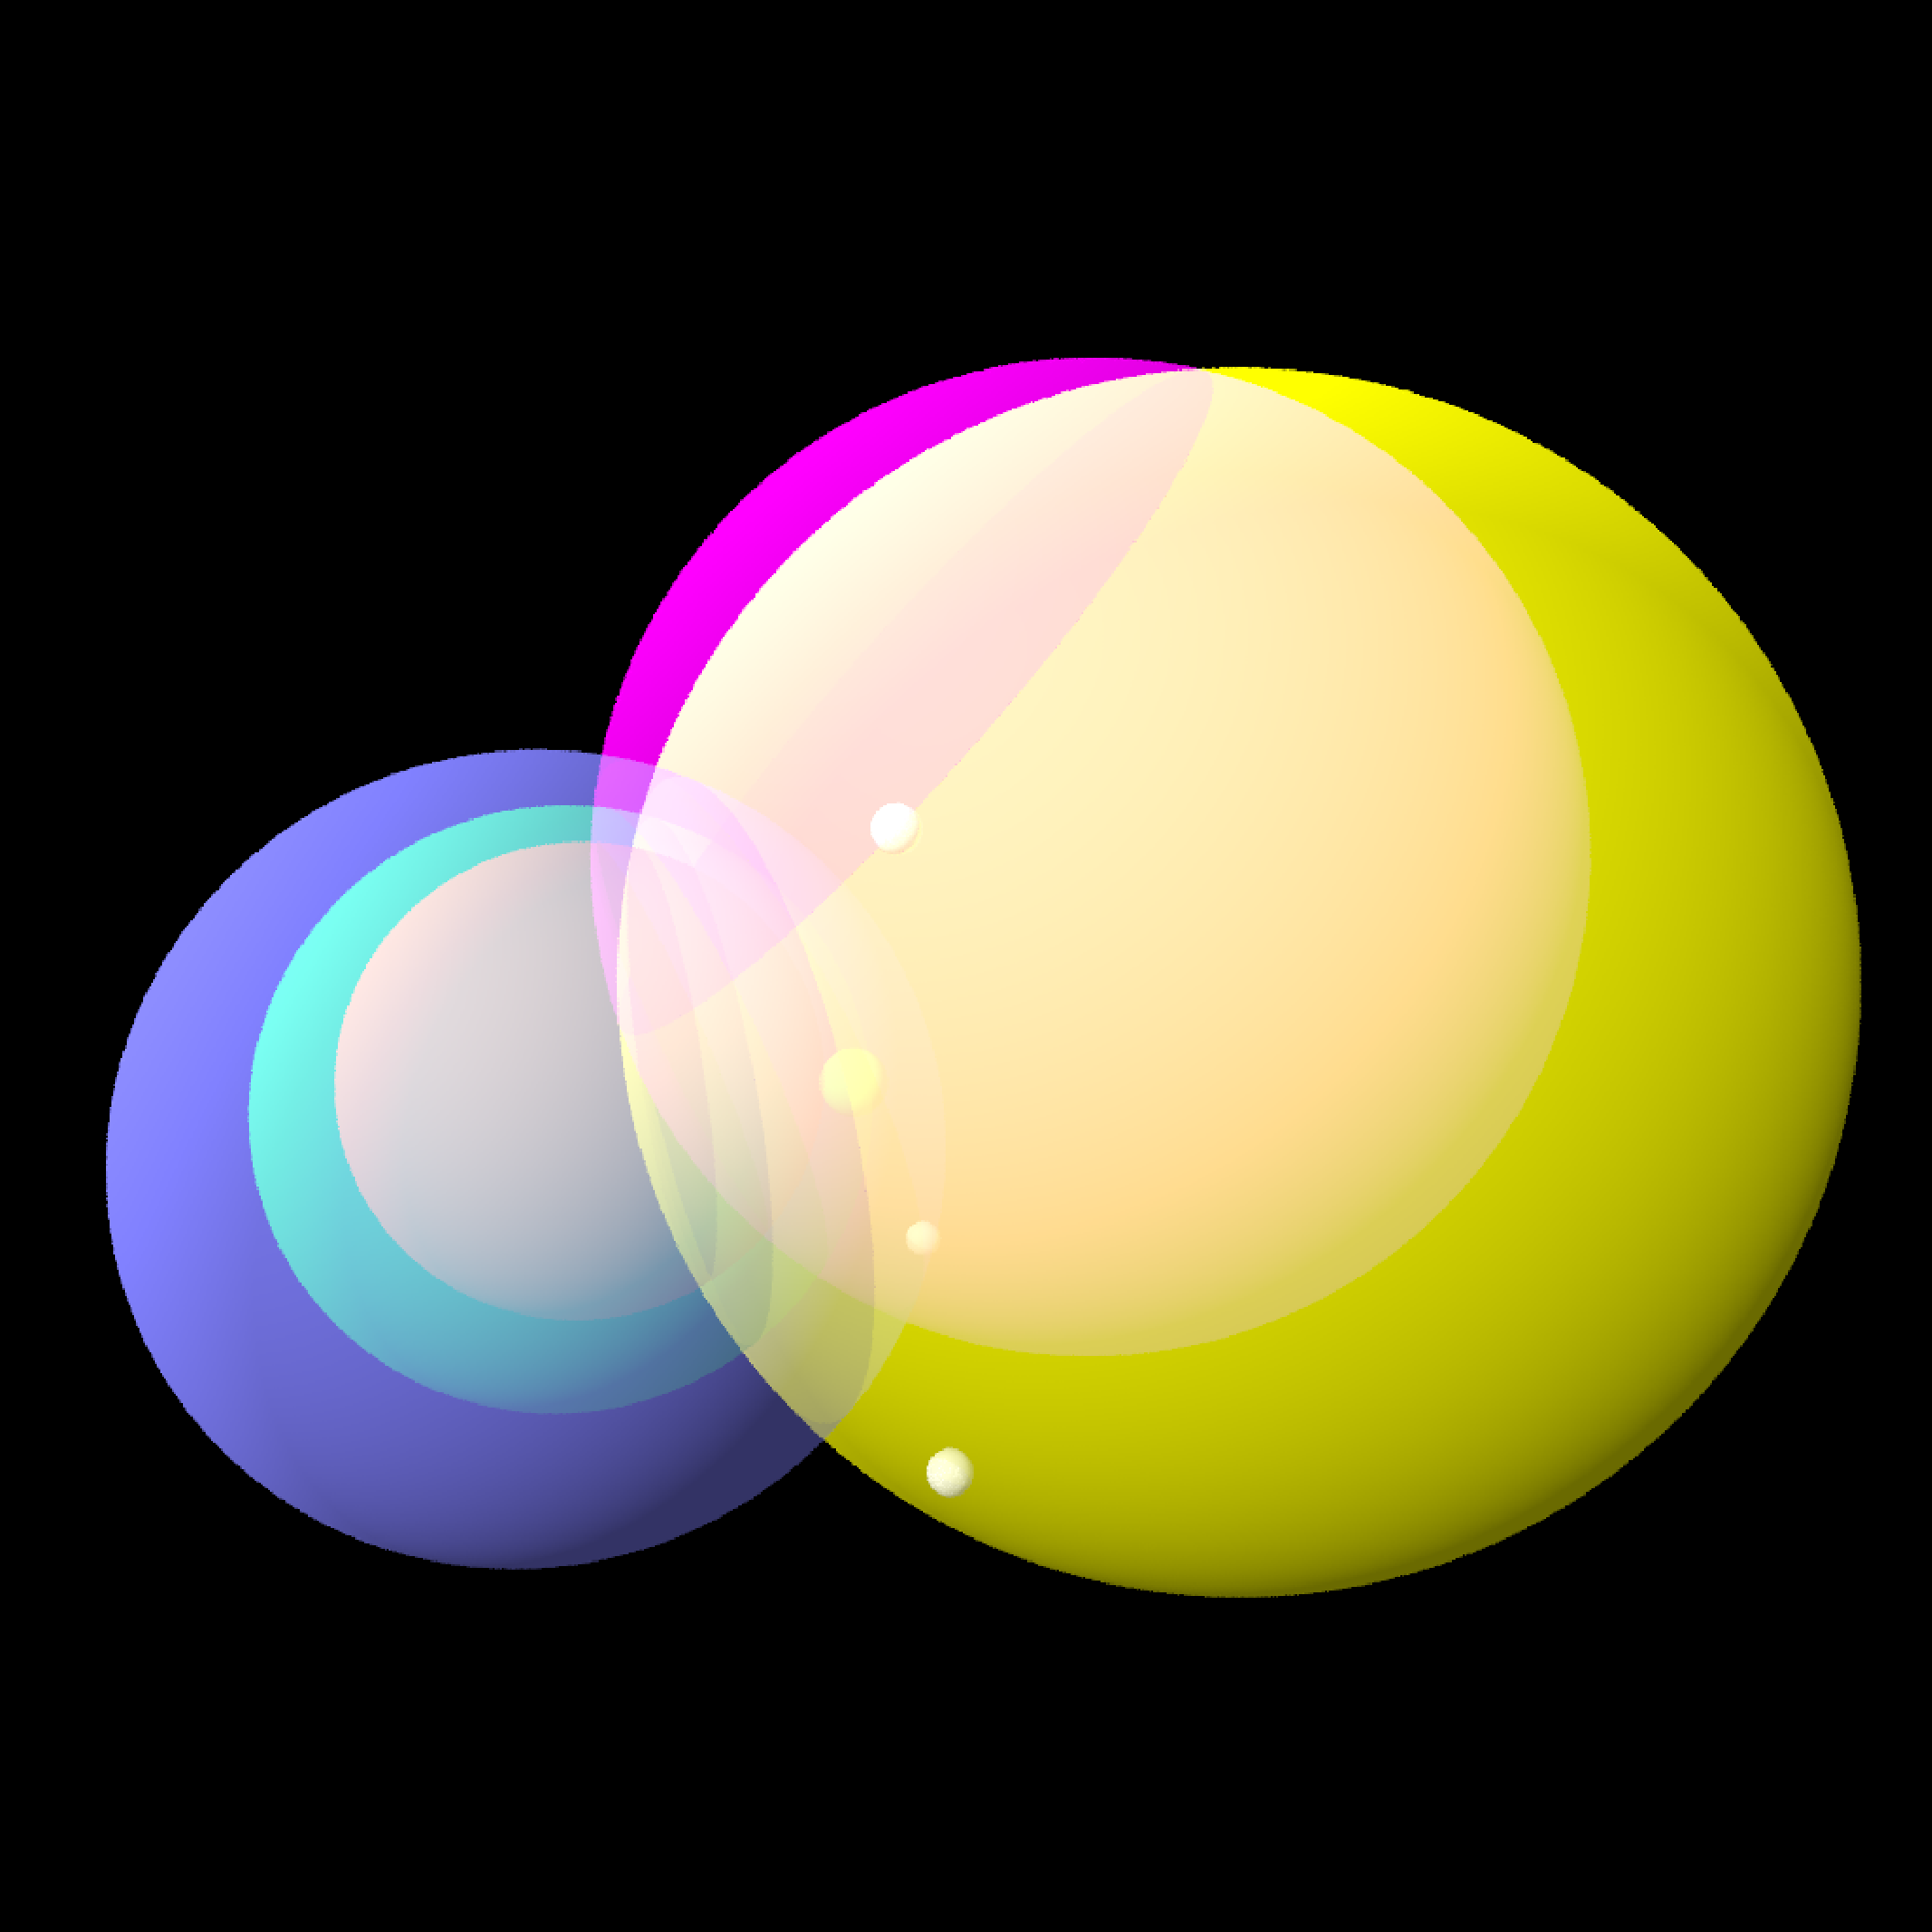
\includegraphics[width=1.4in, height=1.4in, keepaspectratio]{./img/application/3dGen/compLoxoOneGen.pdf}
   \subcaption{\textit{Generator}}
   \label{fig:compLoxoGen}
  \end{minipage}
 \hspace*{\fill}
  \begin{minipage}[t]{0.25\hsize}
   \center
   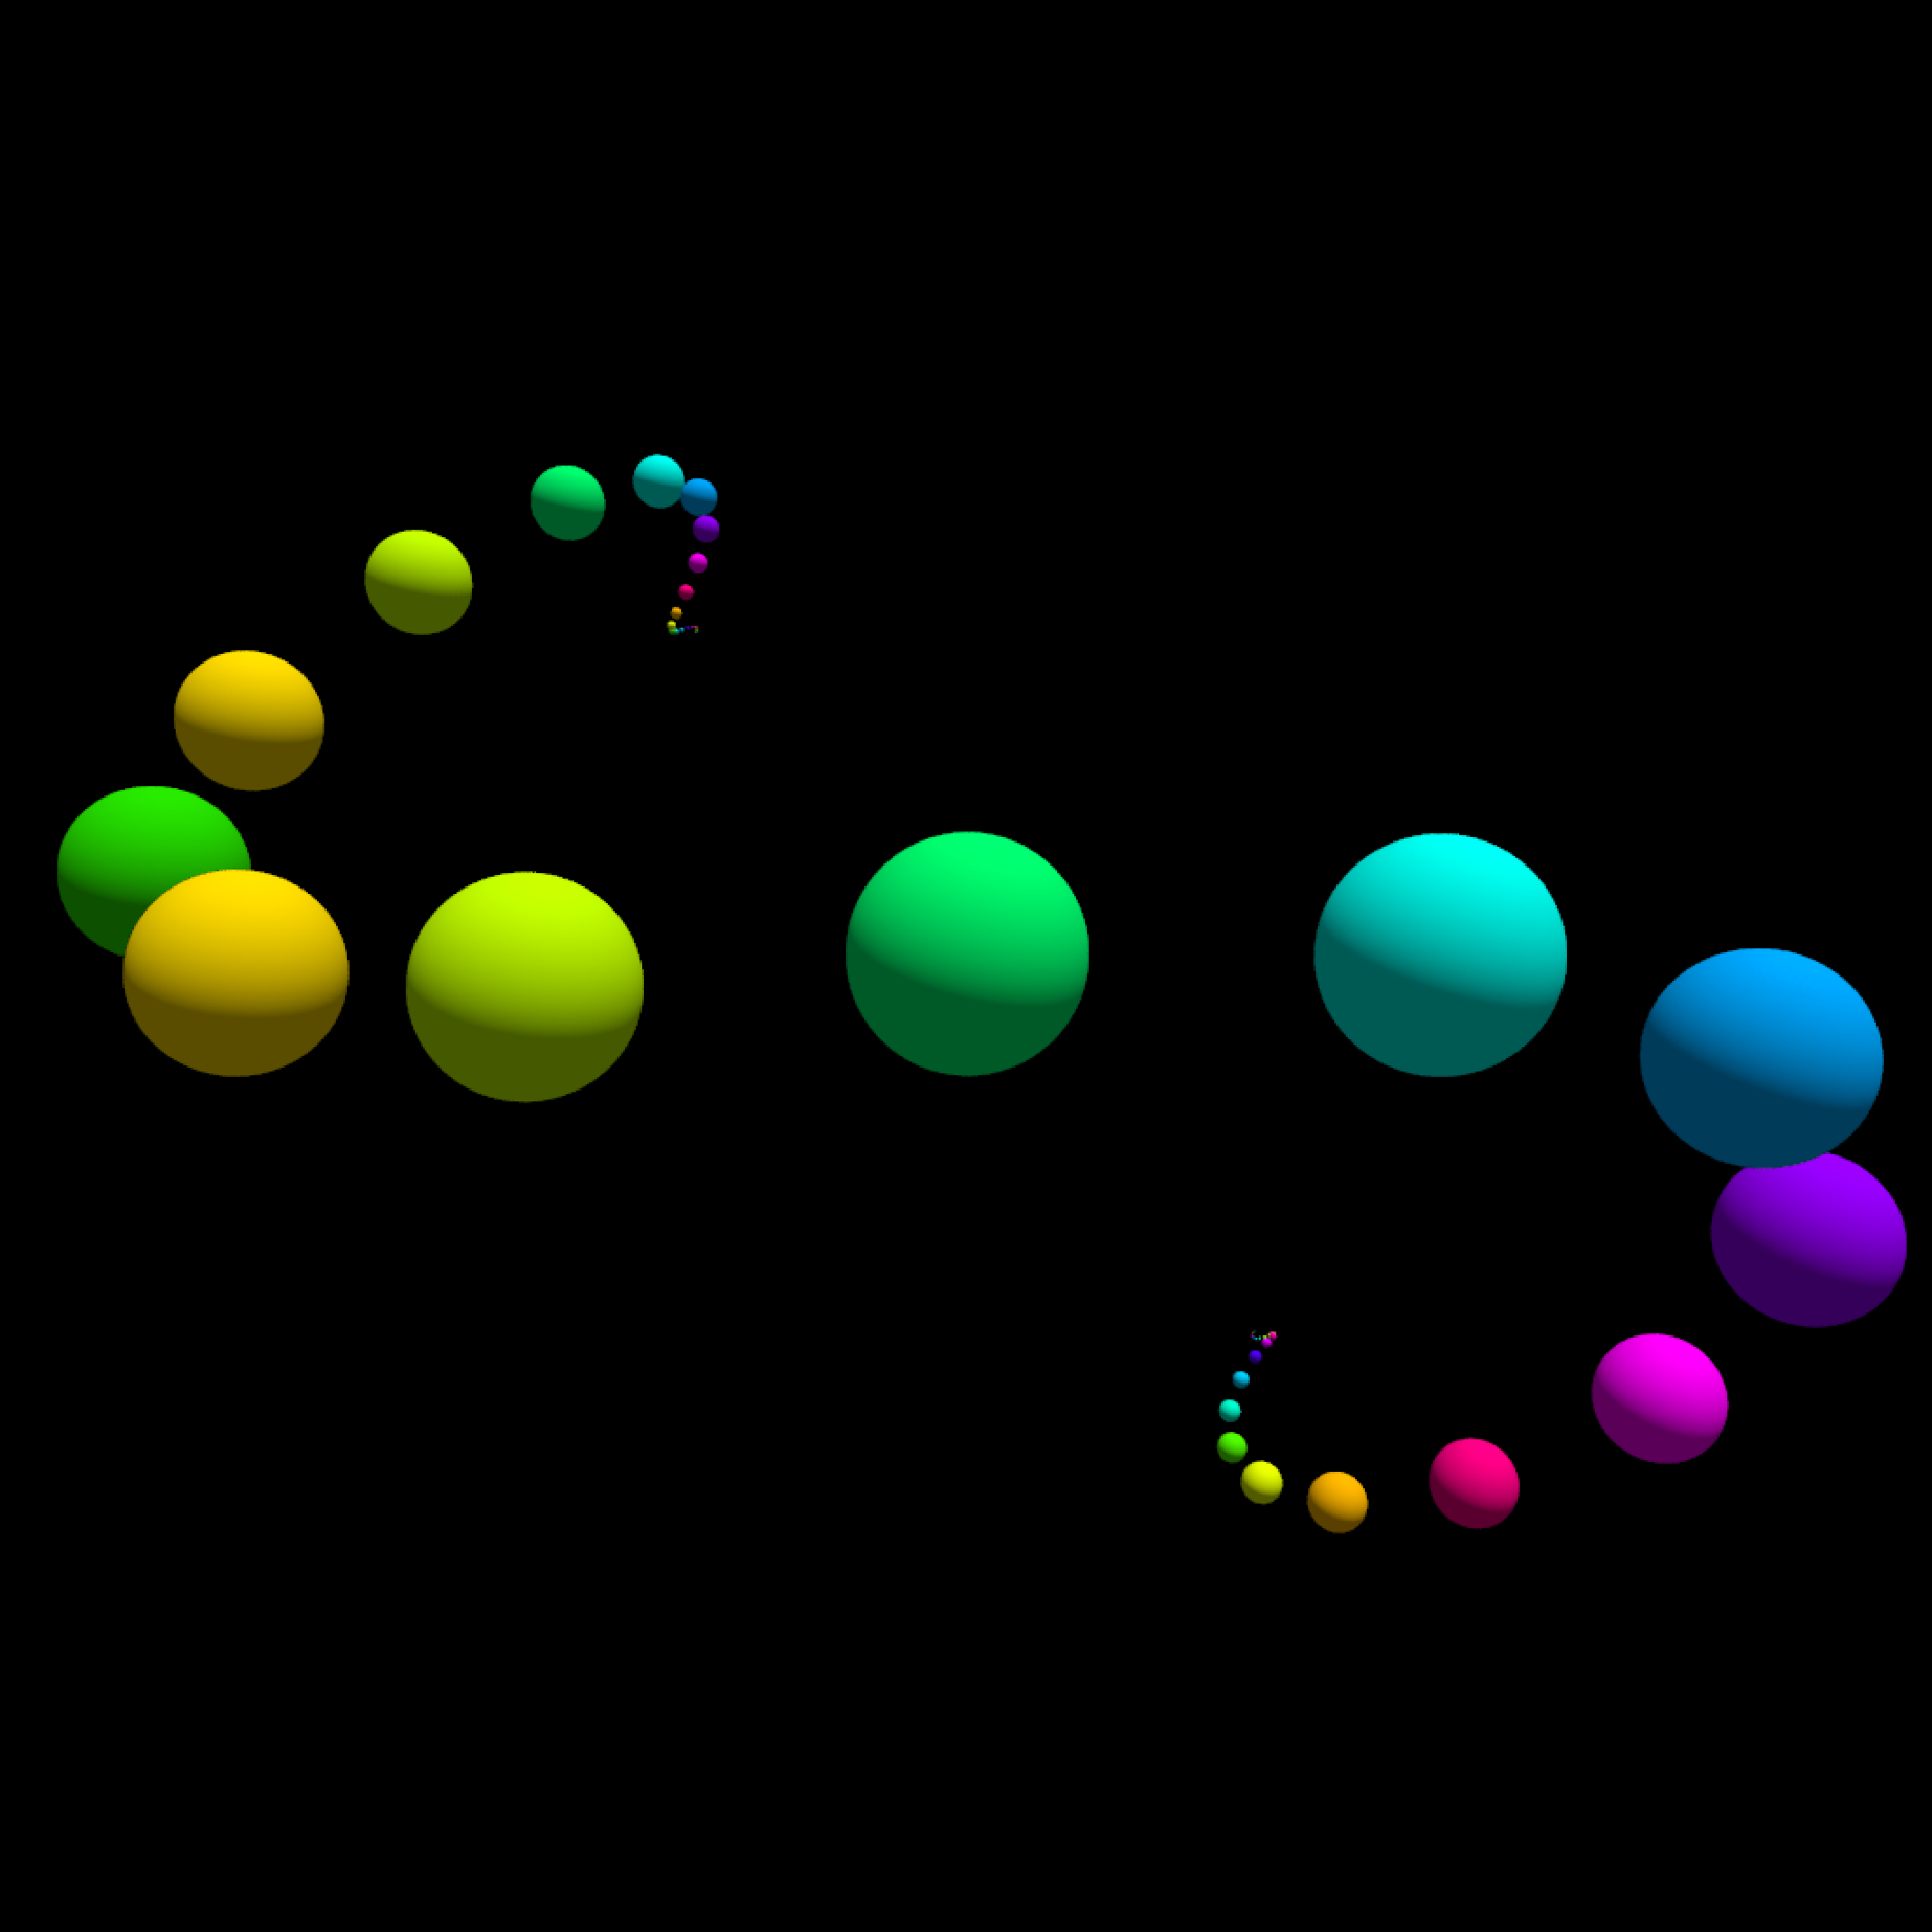
\includegraphics[width=1.4in, height=1.4in, keepaspectratio]{./img/application/3dGen/compLoxoOneOrb.pdf}
   \subcaption{\textit{Orbit}}
   \label{fig:compLoxoOrb}
  \end{minipage}
  \hspace*{\fill}
  \caption{\textit{Compound loxodromic generator and a base sphere}}
  \label{fig:compLoxo}
 \end{minipage}
\end{figure}

\noindent\textbf{Inversion in a Sphere with Infinite Radius.}
An inversion in a sphere with infinite radius is represented by
a reflection through a plane.
See Figure \ref{fig:infSphere}\subref{fig:infSphereGen}.
There are four white inversion spheres, one green base sphere,
and one blue plate.
The blue plate is a part of a sphere with infinite radius.
The orbit of the group is shown in Figure
\ref{fig:infSphere}\subref{fig:infSphereOrb}.
The resulting orbit has a reflection symmetry.

\noindent\textbf{Parallel
Translation~\footnote{\url{https://www.shadertoy.com/view/lsjyzK}}.}
A composition of inversions in two parallel planes represents a parallel
translation along a normal vector of the planes.
See Figure \ref{fig:translation3d}.
This is a parabolic transformation.
Moreover, in 3D, we can add a twist to the orbit.
See Figure \ref{fig:compParabolic}.
The orbit is rotated around the normal vector of the planes for every
translation.
This operation is possible in 3D space, because we have gained a degree
of freedom over 2D space.
The transformations yielding twisted orbits are called \textit{compound
parabolic} transformations.

\noindent\textbf{Rotation.}
A composition of reflections through two crossing planes generates a rotation.
The axis of rotation is the intersection line of two planes.
The generators and the orbit are shown in Figure \ref{fig:rotation3d}.

\noindent\textbf{Composition of Two
Spheres~\footnote{\url{https://www.shadertoy.com/view/ldByDW}}.}
We compose generators using two spheres.
See Figure \ref{fig:loxoGen3d}.
We call the light red sphere $S1$, the light green sphere $S2$, and the blue
sphere $S1'$.
The map $G$ is as follows.
\begin{align*}
G =
\begin{cases}
 I_{S2} \circ I_{S1} & (\text{The point is inside of } S1) \\
 I_{S1} \circ I_{S2} & (\text{The point is outside of }S1')
\end{cases}
\end{align*}
While $S1$ and $S2$ have no intersection, the generator is hyperbolic
transformation.
The orbit of the base sphere is shown in Figure \ref{fig:loxoOrb3d}.
When $S1$ and $S2$ come in contact with each other at one point as shown
in Figure \ref{fig:parabolic3dGen}, it becomes a parabolic transformation.
The orbit of spheres touches at the fixed point.
The orbit is shown in Figure \ref{fig:parabolic3dOrb}.
Also, Figure \ref{fig:complicated3d} shows the example of the more
complicated orbit of spheres generated by adding six Schottky spheres to
the group shown in Figure \ref{fig:loxo3d} and Figure \ref{fig:parabolic3d}.

\noindent\textbf{Compound Loxodromic~\footnote{\url{https://www.shadertoy.com/view/MdjyRV}}.}

\subsection{Sphairahedra and Three-dimensional Fractals}

%% 球面体のタイリングもIISで描画することができる

In 2003, Kazushi Ahara and Yoshiaki Araki invented
\textit{Sphairahedron} to introduce new kind of three dimensional
fractals \cite{ahara2003sphairahedral}.

Sphairahedron is coined word combining two words sphaira- and -hedron.

The fractals are generated by tiling of sphairahedra.

We use IIS for three dimensional tiling.
This method uses 
For more details, read \cite{bridges2018:171}